\documentclass[twoside]{book}

% Packages required by doxygen
\usepackage{fixltx2e}
\usepackage{calc}
\usepackage{doxygen}
\usepackage{graphicx}
\usepackage[utf8]{inputenc}
\usepackage{makeidx}
\usepackage{multicol}
\usepackage{multirow}
\PassOptionsToPackage{warn}{textcomp}
\usepackage{textcomp}
\usepackage[nointegrals]{wasysym}
\usepackage[table]{xcolor}

% Font selection
\usepackage[T1]{fontenc}
\usepackage{mathptmx}
\usepackage[scaled=.90]{helvet}
\usepackage{courier}
\usepackage{amssymb}
\usepackage{sectsty}
\renewcommand{\familydefault}{\sfdefault}
\allsectionsfont{%
  \fontseries{bc}\selectfont%
  \color{darkgray}%
}
\renewcommand{\DoxyLabelFont}{%
  \fontseries{bc}\selectfont%
  \color{darkgray}%
}
\newcommand{\+}{\discretionary{\mbox{\scriptsize$\hookleftarrow$}}{}{}}

% Page & text layout
\usepackage{geometry}
\geometry{%
  a4paper,%
  top=2.5cm,%
  bottom=2.5cm,%
  left=2.5cm,%
  right=2.5cm%
}
\tolerance=750
\hfuzz=15pt
\hbadness=750
\setlength{\emergencystretch}{15pt}
\setlength{\parindent}{0cm}
\setlength{\parskip}{0.2cm}
\makeatletter
\renewcommand{\paragraph}{%
  \@startsection{paragraph}{4}{0ex}{-1.0ex}{1.0ex}{%
    \normalfont\normalsize\bfseries\SS@parafont%
  }%
}
\renewcommand{\subparagraph}{%
  \@startsection{subparagraph}{5}{0ex}{-1.0ex}{1.0ex}{%
    \normalfont\normalsize\bfseries\SS@subparafont%
  }%
}
\makeatother

% Headers & footers
\usepackage{fancyhdr}
\pagestyle{fancyplain}
\fancyhead[LE]{\fancyplain{}{\bfseries\thepage}}
\fancyhead[CE]{\fancyplain{}{}}
\fancyhead[RE]{\fancyplain{}{\bfseries\leftmark}}
\fancyhead[LO]{\fancyplain{}{\bfseries\rightmark}}
\fancyhead[CO]{\fancyplain{}{}}
\fancyhead[RO]{\fancyplain{}{\bfseries\thepage}}
\fancyfoot[LE]{\fancyplain{}{}}
\fancyfoot[CE]{\fancyplain{}{}}
\fancyfoot[RE]{\fancyplain{}{\bfseries\scriptsize Generated on Fri Oct 17 2014 14\+:53\+:11 for smact by Doxygen }}
\fancyfoot[LO]{\fancyplain{}{\bfseries\scriptsize Generated on Fri Oct 17 2014 14\+:53\+:11 for smact by Doxygen }}
\fancyfoot[CO]{\fancyplain{}{}}
\fancyfoot[RO]{\fancyplain{}{}}
\renewcommand{\footrulewidth}{0.4pt}
\renewcommand{\chaptermark}[1]{%
  \markboth{#1}{}%
}
\renewcommand{\sectionmark}[1]{%
  \markright{\thesection\ #1}%
}

% Indices & bibliography
\usepackage{natbib}
\usepackage[titles]{tocloft}
\setcounter{tocdepth}{3}
\setcounter{secnumdepth}{5}
\makeindex

% Hyperlinks (required, but should be loaded last)
\usepackage{ifpdf}
\ifpdf
  \usepackage[pdftex,pagebackref=true]{hyperref}
\else
  \usepackage[ps2pdf,pagebackref=true]{hyperref}
\fi
\hypersetup{%
  colorlinks=true,%
  linkcolor=blue,%
  citecolor=blue,%
  unicode%
}

% Custom commands
\newcommand{\clearemptydoublepage}{%
  \newpage{\pagestyle{empty}\cleardoublepage}%
}


%===== C O N T E N T S =====

\begin{document}

% Titlepage & ToC
\hypersetup{pageanchor=false,
             bookmarks=true,
             bookmarksnumbered=true,
             pdfencoding=unicode
            }
\pagenumbering{roman}
\begin{titlepage}
\vspace*{7cm}
\begin{center}%
{\Large smact }\\
\vspace*{1cm}
{\large Generated by Doxygen 1.8.8}\\
\vspace*{0.5cm}
{\small Fri Oct 17 2014 14:53:11}\\
\end{center}
\end{titlepage}
\clearemptydoublepage
\tableofcontents
\clearemptydoublepage
\pagenumbering{arabic}
\hypersetup{pageanchor=true}

%--- Begin generated contents ---
\chapter{Namespace Index}
\section{Namespace List}
Here is a list of all namespaces with brief descriptions\+:\begin{DoxyCompactList}
\item\contentsline{section}{\hyperlink{namespacesmact}{smact} }{\pageref{namespacesmact}}{}
\item\contentsline{section}{\hyperlink{namespacesmact_1_1builder}{smact.\+builder} }{\pageref{namespacesmact_1_1builder}}{}
\item\contentsline{section}{\hyperlink{namespacesmact_1_1core}{smact.\+core} }{\pageref{namespacesmact_1_1core}}{}
\item\contentsline{section}{\hyperlink{namespacesmact_1_1data}{smact.\+data} }{\pageref{namespacesmact_1_1data}}{}
\item\contentsline{section}{\hyperlink{namespacesmact_1_1distorter}{smact.\+distorter} }{\pageref{namespacesmact_1_1distorter}}{}
\item\contentsline{section}{\hyperlink{namespacesmact_1_1lattice}{smact.\+lattice} }{\pageref{namespacesmact_1_1lattice}}{}
\item\contentsline{section}{\hyperlink{namespacesmact_1_1lattice__parameters}{smact.\+lattice\+\_\+parameters} }{\pageref{namespacesmact_1_1lattice__parameters}}{}
\item\contentsline{section}{\hyperlink{namespacesmact_1_1mainpage}{smact.\+mainpage} }{\pageref{namespacesmact_1_1mainpage}}{}
\item\contentsline{section}{\hyperlink{namespacesmact_1_1parameters}{smact.\+parameters} }{\pageref{namespacesmact_1_1parameters}}{}
\item\contentsline{section}{\hyperlink{namespacesmact_1_1properties}{smact.\+properties} }{\pageref{namespacesmact_1_1properties}}{}
\item\contentsline{section}{\hyperlink{namespacesmact_1_1properties_1_1_band__gap__full}{smact.\+properties.\+Band\+\_\+gap\+\_\+full} }{\pageref{namespacesmact_1_1properties_1_1_band__gap__full}}{}
\item\contentsline{section}{\hyperlink{namespacesmact_1_1properties_1_1_band__gap__simple}{smact.\+properties.\+Band\+\_\+gap\+\_\+simple} }{\pageref{namespacesmact_1_1properties_1_1_band__gap__simple}}{}
\item\contentsline{section}{\hyperlink{namespacesmact_1_1properties_1_1compound__electroneg}{smact.\+properties.\+compound\+\_\+electroneg} }{\pageref{namespacesmact_1_1properties_1_1compound__electroneg}}{}
\item\contentsline{section}{\hyperlink{namespacesmact_1_1properties_1_1compound__electroneg__pauling}{smact.\+properties.\+compound\+\_\+electroneg\+\_\+pauling} }{\pageref{namespacesmact_1_1properties_1_1compound__electroneg__pauling}}{}
\item\contentsline{section}{\hyperlink{namespacesmact_1_1surface}{smact.\+surface} }{\pageref{namespacesmact_1_1surface}}{}
\end{DoxyCompactList}

\chapter{Hierarchical Index}
\section{Class Hierarchy}
This inheritance list is sorted roughly, but not completely, alphabetically\+:\begin{DoxyCompactList}
\item object\begin{DoxyCompactList}
\item \contentsline{section}{smact.\+core.\+Element}{\pageref{classsmact_1_1core_1_1_element}}{}
\begin{DoxyCompactList}
\item \contentsline{section}{smact.\+core.\+Species}{\pageref{classsmact_1_1core_1_1_species}}{}
\end{DoxyCompactList}
\item \contentsline{section}{smact.\+lattice.\+Lattice}{\pageref{classsmact_1_1lattice_1_1_lattice}}{}
\item \contentsline{section}{smact.\+lattice.\+Site}{\pageref{classsmact_1_1lattice_1_1_site}}{}
\end{DoxyCompactList}
\end{DoxyCompactList}

\chapter{Class Index}
\section{Class List}
Here are the classes, structs, unions and interfaces with brief descriptions\+:\begin{DoxyCompactList}
\item\contentsline{section}{\hyperlink{classsmact_1_1core_1_1_element}{smact.\+core.\+Element} }{\pageref{classsmact_1_1core_1_1_element}}{}
\item\contentsline{section}{\hyperlink{classsmact_1_1lattice_1_1_lattice}{smact.\+lattice.\+Lattice} }{\pageref{classsmact_1_1lattice_1_1_lattice}}{}
\item\contentsline{section}{\hyperlink{classsmact_1_1lattice_1_1_site}{smact.\+lattice.\+Site} }{\pageref{classsmact_1_1lattice_1_1_site}}{}
\item\contentsline{section}{\hyperlink{classsmact_1_1core_1_1_species}{smact.\+core.\+Species} }{\pageref{classsmact_1_1core_1_1_species}}{}
\end{DoxyCompactList}

\chapter{File Index}
\section{File List}
Here is a list of all files with brief descriptions\+:\begin{DoxyCompactList}
\item\contentsline{section}{/\+Users/\+K\+T\+B22/\+Source\+Tree/smact/smact/\hyperlink{____init_____8py}{\+\_\+\+\_\+init\+\_\+\+\_\+.\+py} }{\pageref{____init_____8py}}{}
\item\contentsline{section}{/\+Users/\+K\+T\+B22/\+Source\+Tree/smact/smact/\hyperlink{builder_8py}{builder.\+py} }{\pageref{builder_8py}}{}
\item\contentsline{section}{/\+Users/\+K\+T\+B22/\+Source\+Tree/smact/smact/\hyperlink{core_8py}{core.\+py} }{\pageref{core_8py}}{}
\item\contentsline{section}{/\+Users/\+K\+T\+B22/\+Source\+Tree/smact/smact/\hyperlink{data_8py}{data.\+py} }{\pageref{data_8py}}{}
\item\contentsline{section}{/\+Users/\+K\+T\+B22/\+Source\+Tree/smact/smact/\hyperlink{distorter_8py}{distorter.\+py} }{\pageref{distorter_8py}}{}
\item\contentsline{section}{/\+Users/\+K\+T\+B22/\+Source\+Tree/smact/smact/\hyperlink{lattice_8py}{lattice.\+py} }{\pageref{lattice_8py}}{}
\item\contentsline{section}{/\+Users/\+K\+T\+B22/\+Source\+Tree/smact/smact/\hyperlink{lattice__parameters_8py}{lattice\+\_\+parameters.\+py} }{\pageref{lattice__parameters_8py}}{}
\item\contentsline{section}{/\+Users/\+K\+T\+B22/\+Source\+Tree/smact/smact/\hyperlink{mainpage_8py}{mainpage.\+py} }{\pageref{mainpage_8py}}{}
\item\contentsline{section}{/\+Users/\+K\+T\+B22/\+Source\+Tree/smact/smact/\hyperlink{parameters_8py}{parameters.\+py} }{\pageref{parameters_8py}}{}
\item\contentsline{section}{/\+Users/\+K\+T\+B22/\+Source\+Tree/smact/smact/\hyperlink{surface_8py}{surface.\+py} }{\pageref{surface_8py}}{}
\item\contentsline{section}{/\+Users/\+K\+T\+B22/\+Source\+Tree/smact/smact/properties/\hyperlink{properties_2____init_____8py}{\+\_\+\+\_\+init\+\_\+\+\_\+.\+py} }{\pageref{properties_2____init_____8py}}{}
\item\contentsline{section}{/\+Users/\+K\+T\+B22/\+Source\+Tree/smact/smact/properties/\hyperlink{_band__gap__full_8py}{Band\+\_\+gap\+\_\+full.\+py} }{\pageref{_band__gap__full_8py}}{}
\item\contentsline{section}{/\+Users/\+K\+T\+B22/\+Source\+Tree/smact/smact/properties/\hyperlink{_band__gap__simple_8py}{Band\+\_\+gap\+\_\+simple.\+py} }{\pageref{_band__gap__simple_8py}}{}
\item\contentsline{section}{/\+Users/\+K\+T\+B22/\+Source\+Tree/smact/smact/properties/\hyperlink{compound__electroneg_8py}{compound\+\_\+electroneg.\+py} }{\pageref{compound__electroneg_8py}}{}
\item\contentsline{section}{/\+Users/\+K\+T\+B22/\+Source\+Tree/smact/smact/properties/\hyperlink{compound__electroneg__pauling_8py}{compound\+\_\+electroneg\+\_\+pauling.\+py} }{\pageref{compound__electroneg__pauling_8py}}{}
\end{DoxyCompactList}

\chapter{Namespace Documentation}
\hypertarget{namespacesmact}{}\section{smact Namespace Reference}
\label{namespacesmact}\index{smact@{smact}}
\subsection*{Namespaces}
\begin{DoxyCompactItemize}
\item 
 \hyperlink{namespacesmact_1_1builder}{builder}
\item 
 \hyperlink{namespacesmact_1_1core}{core}
\item 
 \hyperlink{namespacesmact_1_1data}{data}
\item 
 \hyperlink{namespacesmact_1_1distorter}{distorter}
\item 
 \hyperlink{namespacesmact_1_1lattice}{lattice}
\item 
 \hyperlink{namespacesmact_1_1lattice__parameters}{lattice\+\_\+parameters}
\item 
 \hyperlink{namespacesmact_1_1parameters}{parameters}
\item 
 \hyperlink{namespacesmact_1_1properties}{properties}
\item 
 \hyperlink{namespacesmact_1_1surface}{surface}
\end{DoxyCompactItemize}

\hypertarget{namespacesmact_1_1builder}{}\section{smact.\+builder Namespace Reference}
\label{namespacesmact_1_1builder}\index{smact.\+builder@{smact.\+builder}}
\subsection*{Functions}
\begin{DoxyCompactItemize}
\item 
def \hyperlink{namespacesmact_1_1builder_a80438d278ab0fd7fc04b82b83f4db074}{cubic\+\_\+perovskite}
\item 
def \hyperlink{namespacesmact_1_1builder_a3f01529c174cbc12e692be61162bc8d7}{wurtzite}
\end{DoxyCompactItemize}


\subsection{Function Documentation}
\hypertarget{namespacesmact_1_1builder_a80438d278ab0fd7fc04b82b83f4db074}{}\index{smact\+::builder@{smact\+::builder}!cubic\+\_\+perovskite@{cubic\+\_\+perovskite}}
\index{cubic\+\_\+perovskite@{cubic\+\_\+perovskite}!smact\+::builder@{smact\+::builder}}
\subsubsection[{cubic\+\_\+perovskite}]{\setlength{\rightskip}{0pt plus 5cm}def smact.\+builder.\+cubic\+\_\+perovskite (
\begin{DoxyParamCaption}
\item[{}]{species, }
\item[{}]{cell\+\_\+par = {\ttfamily \mbox{[}6}, }
\item[{}]{repetitions = {\ttfamily \mbox{[}1}}
\end{DoxyParamCaption}
)}\label{namespacesmact_1_1builder_a80438d278ab0fd7fc04b82b83f4db074}
\hypertarget{namespacesmact_1_1builder_a3f01529c174cbc12e692be61162bc8d7}{}\index{smact\+::builder@{smact\+::builder}!wurtzite@{wurtzite}}
\index{wurtzite@{wurtzite}!smact\+::builder@{smact\+::builder}}
\subsubsection[{wurtzite}]{\setlength{\rightskip}{0pt plus 5cm}def smact.\+builder.\+wurtzite (
\begin{DoxyParamCaption}
\item[{}]{species, }
\item[{}]{cell\+\_\+par = {\ttfamily \mbox{[}2}, }
\item[{}]{repetitions = {\ttfamily \mbox{[}1}}
\end{DoxyParamCaption}
)}\label{namespacesmact_1_1builder_a3f01529c174cbc12e692be61162bc8d7}

\hypertarget{namespacesmact_1_1core}{}\section{smact.\+core Namespace Reference}
\label{namespacesmact_1_1core}\index{smact.\+core@{smact.\+core}}
\subsection*{Classes}
\begin{DoxyCompactItemize}
\item 
class \hyperlink{classsmact_1_1core_1_1_element}{Element}
\item 
class \hyperlink{classsmact_1_1core_1_1_species}{Species}
\end{DoxyCompactItemize}
\subsection*{Functions}
\begin{DoxyCompactItemize}
\item 
def \hyperlink{namespacesmact_1_1core_a3e8b27f822e17a79e50b1399825564ff}{ordered\+\_\+elements}
\item 
def \hyperlink{namespacesmact_1_1core_a5a32e4b9b50d3db379ede8d7b8b1081a}{are\+\_\+eq}
\item 
def \hyperlink{namespacesmact_1_1core_abd4953dbc9b28e11861b3b63092ec4fa}{lattices\+\_\+are\+\_\+same}
\item 
def \hyperlink{namespacesmact_1_1core_a523386aa44322d0a2670672b4535bab3}{charge\+\_\+neutrality}
\end{DoxyCompactItemize}
\subsection*{Variables}
\begin{DoxyCompactItemize}
\item 
tuple \hyperlink{namespacesmact_1_1core_aaa14f990a82d90eaab5ad3667e72453e}{smact\+\_\+directory} = os.\+path.\+dirname(\+\_\+\+\_\+file\+\_\+\+\_\+)
\end{DoxyCompactItemize}


\subsection{Function Documentation}
\hypertarget{namespacesmact_1_1core_a5a32e4b9b50d3db379ede8d7b8b1081a}{}\index{smact\+::core@{smact\+::core}!are\+\_\+eq@{are\+\_\+eq}}
\index{are\+\_\+eq@{are\+\_\+eq}!smact\+::core@{smact\+::core}}
\subsubsection[{are\+\_\+eq}]{\setlength{\rightskip}{0pt plus 5cm}def smact.\+core.\+are\+\_\+eq (
\begin{DoxyParamCaption}
\item[{}]{A, }
\item[{}]{B, }
\item[{}]{tolerance = {\ttfamily 1e-\/4}}
\end{DoxyParamCaption}
)}\label{namespacesmact_1_1core_a5a32e4b9b50d3db379ede8d7b8b1081a}
\begin{DoxyVerb}Check two arrays for tolerance [1,2,3]==[1,2,3]; but [1,3,2]!=[1,2,3]
    Args:
    A/B: arrays
    tolerance: numerical precision for equality condition
    Returns:
    True/False
\end{DoxyVerb}
 \hypertarget{namespacesmact_1_1core_a523386aa44322d0a2670672b4535bab3}{}\index{smact\+::core@{smact\+::core}!charge\+\_\+neutrality@{charge\+\_\+neutrality}}
\index{charge\+\_\+neutrality@{charge\+\_\+neutrality}!smact\+::core@{smact\+::core}}
\subsubsection[{charge\+\_\+neutrality}]{\setlength{\rightskip}{0pt plus 5cm}def smact.\+core.\+charge\+\_\+neutrality (
\begin{DoxyParamCaption}
\item[{}]{oxidations, }
\item[{}]{stoichs = {\ttfamily False}, }
\item[{}]{threshold = {\ttfamily 5}}
\end{DoxyParamCaption}
)}\label{namespacesmact_1_1core_a523386aa44322d0a2670672b4535bab3}
\begin{DoxyVerb}Given a list of oxidation states of arbitrary length it serches for neutral ratios in a given ratio of sites (stoichs) or up to a given threshold
   For the moment it just iterates through binaries, ternaries ... TODO: make it general (KTB)
Args:
oxidations : list of integers
stoichs : stoichiometric ratios for each site (if provided)
threshold : single threshold to go up to if stoichs are not provided
Returns:
exists : bool to say if a ratio exists
site_ratios : ration that gives neutrality
\end{DoxyVerb}
 \hypertarget{namespacesmact_1_1core_abd4953dbc9b28e11861b3b63092ec4fa}{}\index{smact\+::core@{smact\+::core}!lattices\+\_\+are\+\_\+same@{lattices\+\_\+are\+\_\+same}}
\index{lattices\+\_\+are\+\_\+same@{lattices\+\_\+are\+\_\+same}!smact\+::core@{smact\+::core}}
\subsubsection[{lattices\+\_\+are\+\_\+same}]{\setlength{\rightskip}{0pt plus 5cm}def smact.\+core.\+lattices\+\_\+are\+\_\+same (
\begin{DoxyParamCaption}
\item[{}]{lattice1, }
\item[{}]{lattice2}
\end{DoxyParamCaption}
)}\label{namespacesmact_1_1core_abd4953dbc9b28e11861b3b63092ec4fa}
\begin{DoxyVerb}Checks for the equivalence of two lattices
    Args:
    lattice1,lattice2 : ASE crystal class
    Returns:
    lattices_are_same : boolean \end{DoxyVerb}
 \hypertarget{namespacesmact_1_1core_a3e8b27f822e17a79e50b1399825564ff}{}\index{smact\+::core@{smact\+::core}!ordered\+\_\+elements@{ordered\+\_\+elements}}
\index{ordered\+\_\+elements@{ordered\+\_\+elements}!smact\+::core@{smact\+::core}}
\subsubsection[{ordered\+\_\+elements}]{\setlength{\rightskip}{0pt plus 5cm}def smact.\+core.\+ordered\+\_\+elements (
\begin{DoxyParamCaption}
\item[{}]{x, }
\item[{}]{y}
\end{DoxyParamCaption}
)}\label{namespacesmact_1_1core_a3e8b27f822e17a79e50b1399825564ff}
\begin{DoxyVerb}Function to return a list of element symbols, ordered by proton number in the range x -> y
Args:
x,y : integers
Returns:
ordered_elements : List of element symbols
\end{DoxyVerb}
 

\subsection{Variable Documentation}
\hypertarget{namespacesmact_1_1core_aaa14f990a82d90eaab5ad3667e72453e}{}\index{smact\+::core@{smact\+::core}!smact\+\_\+directory@{smact\+\_\+directory}}
\index{smact\+\_\+directory@{smact\+\_\+directory}!smact\+::core@{smact\+::core}}
\subsubsection[{smact\+\_\+directory}]{\setlength{\rightskip}{0pt plus 5cm}string smact.\+core.\+smact\+\_\+directory = os.\+path.\+dirname(\+\_\+\+\_\+file\+\_\+\+\_\+)}\label{namespacesmact_1_1core_aaa14f990a82d90eaab5ad3667e72453e}

\hypertarget{namespacesmact_1_1data}{}\section{smact.\+data Namespace Reference}
\label{namespacesmact_1_1data}\index{smact.\+data@{smact.\+data}}
\subsection*{Functions}
\begin{DoxyCompactItemize}
\item 
def \hyperlink{namespacesmact_1_1data_a2cb4d9dded3d65889eff3badac947922}{get\+\_\+mulliken}
\begin{DoxyCompactList}\small\item\em Copyright Daniel Davies, Adam J. \end{DoxyCompactList}\item 
def \hyperlink{namespacesmact_1_1data_a5777f26050189e84aff07dff82185d05}{get\+\_\+pauling}
\begin{DoxyCompactList}\small\item\em The following functions are deprecated. \end{DoxyCompactList}\item 
def \hyperlink{namespacesmact_1_1data_a99f38b1d5bd7e101330f88fd1aedb794}{get\+\_\+covalent}
\item 
def \hyperlink{namespacesmact_1_1data_af25e690defd2aa1923b815cb5eb73ca6}{get\+\_\+eig}
\item 
def \hyperlink{namespacesmact_1_1data_a80cf4a9c06413608e98a6086dbedb87b}{get\+\_\+eig\+\_\+s}
\item 
def \hyperlink{namespacesmact_1_1data_a5249c4b761aa5c3a2d06dabdac2fafbf}{get\+\_\+ionic}
\end{DoxyCompactItemize}


\subsection{Function Documentation}
\hypertarget{namespacesmact_1_1data_a99f38b1d5bd7e101330f88fd1aedb794}{}\index{smact\+::data@{smact\+::data}!get\+\_\+covalent@{get\+\_\+covalent}}
\index{get\+\_\+covalent@{get\+\_\+covalent}!smact\+::data@{smact\+::data}}
\subsubsection[{get\+\_\+covalent}]{\setlength{\rightskip}{0pt plus 5cm}def smact.\+data.\+get\+\_\+covalent (
\begin{DoxyParamCaption}
\item[{}]{symbol}
\end{DoxyParamCaption}
)}\label{namespacesmact_1_1data_a99f38b1d5bd7e101330f88fd1aedb794}
\begin{DoxyVerb}Covalent radius of specified element.
Drawn from Open Babel data table.\end{DoxyVerb}
 \hypertarget{namespacesmact_1_1data_af25e690defd2aa1923b815cb5eb73ca6}{}\index{smact\+::data@{smact\+::data}!get\+\_\+eig@{get\+\_\+eig}}
\index{get\+\_\+eig@{get\+\_\+eig}!smact\+::data@{smact\+::data}}
\subsubsection[{get\+\_\+eig}]{\setlength{\rightskip}{0pt plus 5cm}def smact.\+data.\+get\+\_\+eig (
\begin{DoxyParamCaption}
\item[{}]{symbol}
\end{DoxyParamCaption}
)}\label{namespacesmact_1_1data_af25e690defd2aa1923b815cb5eb73ca6}
\hypertarget{namespacesmact_1_1data_a80cf4a9c06413608e98a6086dbedb87b}{}\index{smact\+::data@{smact\+::data}!get\+\_\+eig\+\_\+s@{get\+\_\+eig\+\_\+s}}
\index{get\+\_\+eig\+\_\+s@{get\+\_\+eig\+\_\+s}!smact\+::data@{smact\+::data}}
\subsubsection[{get\+\_\+eig\+\_\+s}]{\setlength{\rightskip}{0pt plus 5cm}def smact.\+data.\+get\+\_\+eig\+\_\+s (
\begin{DoxyParamCaption}
\item[{}]{symbol}
\end{DoxyParamCaption}
)}\label{namespacesmact_1_1data_a80cf4a9c06413608e98a6086dbedb87b}
\hypertarget{namespacesmact_1_1data_a5249c4b761aa5c3a2d06dabdac2fafbf}{}\index{smact\+::data@{smact\+::data}!get\+\_\+ionic@{get\+\_\+ionic}}
\index{get\+\_\+ionic@{get\+\_\+ionic}!smact\+::data@{smact\+::data}}
\subsubsection[{get\+\_\+ionic}]{\setlength{\rightskip}{0pt plus 5cm}def smact.\+data.\+get\+\_\+ionic (
\begin{DoxyParamCaption}
\item[{}]{symbol}
\end{DoxyParamCaption}
)}\label{namespacesmact_1_1data_a5249c4b761aa5c3a2d06dabdac2fafbf}
\hypertarget{namespacesmact_1_1data_a2cb4d9dded3d65889eff3badac947922}{}\index{smact\+::data@{smact\+::data}!get\+\_\+mulliken@{get\+\_\+mulliken}}
\index{get\+\_\+mulliken@{get\+\_\+mulliken}!smact\+::data@{smact\+::data}}
\subsubsection[{get\+\_\+mulliken}]{\setlength{\rightskip}{0pt plus 5cm}def smact.\+data.\+get\+\_\+mulliken (
\begin{DoxyParamCaption}
\item[{}]{symbol}
\end{DoxyParamCaption}
)}\label{namespacesmact_1_1data_a2cb4d9dded3d65889eff3badac947922}


Copyright Daniel Davies, Adam J. 

Jackson (2013) \# \# This file is part of S\+M\+A\+C\+T\+: \hyperlink{data_8py}{data.\+py} is free software\+: you can \# redistribute it and/or modify it under the terms of the G\+N\+U General Public \# License as published by the Free Software Foundation, either version 3 of \# the License, or (at your option) any later version. \# This program is distributed in the hope that it will be useful, but W\+I\+T\+H\+O\+U\+T \# A\+N\+Y W\+A\+R\+R\+A\+N\+T\+Y; without even the implied warranty of M\+E\+R\+C\+H\+A\+N\+T\+A\+B\+I\+L\+I\+T\+Y or \# F\+I\+T\+N\+E\+S\+S F\+O\+R A P\+A\+R\+T\+I\+C\+U\+L\+A\+R P\+U\+R\+P\+O\+S\+E. See the G\+N\+U General Public License for \# more details. \# You should have received a copy of the G\+N\+U General Public License along with\# this program. If not, see \href{http://www.gnu.org/licenses/}{\tt http\+://www.\+gnu.\+org/licenses/}. \#\begin{DoxyVerb}Gets Mulliken electroneg from the IE and EA\end{DoxyVerb}
 \hypertarget{namespacesmact_1_1data_a5777f26050189e84aff07dff82185d05}{}\index{smact\+::data@{smact\+::data}!get\+\_\+pauling@{get\+\_\+pauling}}
\index{get\+\_\+pauling@{get\+\_\+pauling}!smact\+::data@{smact\+::data}}
\subsubsection[{get\+\_\+pauling}]{\setlength{\rightskip}{0pt plus 5cm}def smact.\+data.\+get\+\_\+pauling (
\begin{DoxyParamCaption}
\item[{}]{symbol}
\end{DoxyParamCaption}
)}\label{namespacesmact_1_1data_a5777f26050189e84aff07dff82185d05}


The following functions are deprecated. 

New code should access these \#\#\#\# properties directly by forming an \char`\"{}element\char`\"{} object and calling the \#\#\#\# desired property, as in the wrappers below. \#\#\#\#\begin{DoxyVerb}Pauling electronegativity of specified element.
Drawn from Open Babel data table.\end{DoxyVerb}
 
\hypertarget{namespacesmact_1_1distorter}{}\section{smact.\+distorter Namespace Reference}
\label{namespacesmact_1_1distorter}\index{smact.\+distorter@{smact.\+distorter}}
\subsection*{Functions}
\begin{DoxyCompactItemize}
\item 
def \hyperlink{namespacesmact_1_1distorter_a0ac75ed2f6cb305b3c8596d94517eec6}{get\+\_\+sg}
\item 
def \hyperlink{namespacesmact_1_1distorter_a1ec14de462a0176842705f8fc4c9c39b}{get\+\_\+inequivalent\+\_\+sites}
\item 
def \hyperlink{namespacesmact_1_1distorter_ade340d55f2d7f76740c01bbc79e3be91}{make\+\_\+substitution}
\item 
def \hyperlink{namespacesmact_1_1distorter_a39d7cc60d45b249ab88edc3ec929e68b}{build\+\_\+sub\+\_\+lattice}
\end{DoxyCompactItemize}


\subsection{Function Documentation}
\hypertarget{namespacesmact_1_1distorter_a39d7cc60d45b249ab88edc3ec929e68b}{}\index{smact\+::distorter@{smact\+::distorter}!build\+\_\+sub\+\_\+lattice@{build\+\_\+sub\+\_\+lattice}}
\index{build\+\_\+sub\+\_\+lattice@{build\+\_\+sub\+\_\+lattice}!smact\+::distorter@{smact\+::distorter}}
\subsubsection[{build\+\_\+sub\+\_\+lattice}]{\setlength{\rightskip}{0pt plus 5cm}def smact.\+distorter.\+build\+\_\+sub\+\_\+lattice (
\begin{DoxyParamCaption}
\item[{}]{lattice, }
\item[{}]{symbol}
\end{DoxyParamCaption}
)}\label{namespacesmact_1_1distorter_a39d7cc60d45b249ab88edc3ec929e68b}
\begin{DoxyVerb}Generate a sub-lattice of the lattice based on equivalent atomic species

Args:
    lattice: ASE crystal class
symbol: The name of the species whose sub-lattice you wish to build

Returns:
sub_lattice: Cartesian coordinates of the sub-lattice of symbol\end{DoxyVerb}
 \hypertarget{namespacesmact_1_1distorter_a1ec14de462a0176842705f8fc4c9c39b}{}\index{smact\+::distorter@{smact\+::distorter}!get\+\_\+inequivalent\+\_\+sites@{get\+\_\+inequivalent\+\_\+sites}}
\index{get\+\_\+inequivalent\+\_\+sites@{get\+\_\+inequivalent\+\_\+sites}!smact\+::distorter@{smact\+::distorter}}
\subsubsection[{get\+\_\+inequivalent\+\_\+sites}]{\setlength{\rightskip}{0pt plus 5cm}def smact.\+distorter.\+get\+\_\+inequivalent\+\_\+sites (
\begin{DoxyParamCaption}
\item[{}]{sub\+\_\+lattice, }
\item[{}]{lattice}
\end{DoxyParamCaption}
)}\label{namespacesmact_1_1distorter_a1ec14de462a0176842705f8fc4c9c39b}
\begin{DoxyVerb}Given a sub lattice, returns symmetry unique sites for substitutions

Args:
sub_lattice: array containing Cartesian coordinates of the sub-lattice of interest
lattice: ASE crystal class, the total lattice\end{DoxyVerb}
 \hypertarget{namespacesmact_1_1distorter_a0ac75ed2f6cb305b3c8596d94517eec6}{}\index{smact\+::distorter@{smact\+::distorter}!get\+\_\+sg@{get\+\_\+sg}}
\index{get\+\_\+sg@{get\+\_\+sg}!smact\+::distorter@{smact\+::distorter}}
\subsubsection[{get\+\_\+sg}]{\setlength{\rightskip}{0pt plus 5cm}def smact.\+distorter.\+get\+\_\+sg (
\begin{DoxyParamCaption}
\item[{}]{lattice}
\end{DoxyParamCaption}
)}\label{namespacesmact_1_1distorter_a0ac75ed2f6cb305b3c8596d94517eec6}
\begin{DoxyVerb}Get the space-group of the system

Args:
lattice: the ASE crystal class
Returns:
sg: integer number of the spacegroup\end{DoxyVerb}
 \hypertarget{namespacesmact_1_1distorter_ade340d55f2d7f76740c01bbc79e3be91}{}\index{smact\+::distorter@{smact\+::distorter}!make\+\_\+substitution@{make\+\_\+substitution}}
\index{make\+\_\+substitution@{make\+\_\+substitution}!smact\+::distorter@{smact\+::distorter}}
\subsubsection[{make\+\_\+substitution}]{\setlength{\rightskip}{0pt plus 5cm}def smact.\+distorter.\+make\+\_\+substitution (
\begin{DoxyParamCaption}
\item[{}]{lattice, }
\item[{}]{site, }
\item[{}]{new\+\_\+species}
\end{DoxyParamCaption}
)}\label{namespacesmact_1_1distorter_ade340d55f2d7f76740c01bbc79e3be91}
\begin{DoxyVerb}Change the atomic species @ site in lattice to new_species [atomic number]

Args:
lattice: ASE crystal class
site: array, containing the Cartesian coordinates of the substitution site
new_species: string, the new species\end{DoxyVerb}
 
\hypertarget{namespacesmact_1_1lattice}{}\section{smact.\+lattice Namespace Reference}
\label{namespacesmact_1_1lattice}\index{smact.\+lattice@{smact.\+lattice}}
\subsection*{Classes}
\begin{DoxyCompactItemize}
\item 
class \hyperlink{classsmact_1_1lattice_1_1_lattice}{Lattice}
\item 
class \hyperlink{classsmact_1_1lattice_1_1_site}{Site}
\end{DoxyCompactItemize}
\subsection*{Functions}
\begin{DoxyCompactItemize}
\item 
def \hyperlink{namespacesmact_1_1lattice_a0380cf2cee37daa74c90bbefa4a16246}{check\+\_\+lattice\+\_\+charges}
\item 
def \hyperlink{namespacesmact_1_1lattice_af33a880afcb916626bc20669a084457f}{possible\+\_\+compositions}
\item 
def \hyperlink{namespacesmact_1_1lattice_a480b77e0ed0d4874c376d27f41ee0b3c}{possible\+\_\+elements}
\end{DoxyCompactItemize}


\subsection{Function Documentation}
\hypertarget{namespacesmact_1_1lattice_a0380cf2cee37daa74c90bbefa4a16246}{}\index{smact\+::lattice@{smact\+::lattice}!check\+\_\+lattice\+\_\+charges@{check\+\_\+lattice\+\_\+charges}}
\index{check\+\_\+lattice\+\_\+charges@{check\+\_\+lattice\+\_\+charges}!smact\+::lattice@{smact\+::lattice}}
\subsubsection[{check\+\_\+lattice\+\_\+charges}]{\setlength{\rightskip}{0pt plus 5cm}def smact.\+lattice.\+check\+\_\+lattice\+\_\+charges (
\begin{DoxyParamCaption}
\item[{}]{charges, }
\item[{}]{site\+\_\+elements, }
\item[{}]{sites}
\end{DoxyParamCaption}
)}\label{namespacesmact_1_1lattice_a0380cf2cee37daa74c90bbefa4a16246}
\begin{DoxyVerb}This function checks the sum of the charges on the lattice sites in the crystal
Additional explanation if needed

Args:
    charges: array of the charge contributions of each lattice site
    site_elements: All possible elements which satisfy charge neutrality 
    sites: list, the current set of elements under inspection

Returns:
    input site_elements array with appended neutral sites (???)\end{DoxyVerb}
 \hypertarget{namespacesmact_1_1lattice_af33a880afcb916626bc20669a084457f}{}\index{smact\+::lattice@{smact\+::lattice}!possible\+\_\+compositions@{possible\+\_\+compositions}}
\index{possible\+\_\+compositions@{possible\+\_\+compositions}!smact\+::lattice@{smact\+::lattice}}
\subsubsection[{possible\+\_\+compositions}]{\setlength{\rightskip}{0pt plus 5cm}def smact.\+lattice.\+possible\+\_\+compositions (
\begin{DoxyParamCaption}
\item[{}]{crystal, }
\item[{}]{elements}
\end{DoxyParamCaption}
)}\label{namespacesmact_1_1lattice_af33a880afcb916626bc20669a084457f}
\begin{DoxyVerb}Seach for the elements which satisfy the possible oxidations and charge neutrality.

Args:
    crystal: A Lattice object defining the crystal class
    elements: A list of the elemets you wish to search through
Uses:
atom : a list of possible atoms on each site of the lattice
Returns:
    list/array/dict of int/float/string of something useful (???)
\end{DoxyVerb}
 \hypertarget{namespacesmact_1_1lattice_a480b77e0ed0d4874c376d27f41ee0b3c}{}\index{smact\+::lattice@{smact\+::lattice}!possible\+\_\+elements@{possible\+\_\+elements}}
\index{possible\+\_\+elements@{possible\+\_\+elements}!smact\+::lattice@{smact\+::lattice}}
\subsubsection[{possible\+\_\+elements}]{\setlength{\rightskip}{0pt plus 5cm}def smact.\+lattice.\+possible\+\_\+elements (
\begin{DoxyParamCaption}
\item[{}]{elements, }
\item[{}]{oxidations}
\end{DoxyParamCaption}
)}\label{namespacesmact_1_1lattice_a480b77e0ed0d4874c376d27f41ee0b3c}
\begin{DoxyVerb}Identify possible atoms to occupy a site

Args:
    elements:
    oxidations: 

Returns: 
    Array of atoms\end{DoxyVerb}
 
\hypertarget{namespacesmact_1_1lattice__parameters}{}\section{smact.\+lattice\+\_\+parameters Namespace Reference}
\label{namespacesmact_1_1lattice__parameters}\index{smact.\+lattice\+\_\+parameters@{smact.\+lattice\+\_\+parameters}}
\subsection*{Functions}
\begin{DoxyCompactItemize}
\item 
def \hyperlink{namespacesmact_1_1lattice__parameters_ad362e3a76b00a5dad0aab8ec370525d4}{cubic\+\_\+perovskite}
\item 
def \hyperlink{namespacesmact_1_1lattice__parameters_ad9f584d4e062d087e18aeca194c2537b}{wurtzite}
\item 
def \hyperlink{namespacesmact_1_1lattice__parameters_a4e67c0acfd178548e38a8ae341791259}{fcc}
\item 
def \hyperlink{namespacesmact_1_1lattice__parameters_a797eec432832ec55c5da86125c120779}{bcc}
\item 
def \hyperlink{namespacesmact_1_1lattice__parameters_a09030d3085ef12b8a3d03ce1f1ebc3d0}{hcp}
\item 
def \hyperlink{namespacesmact_1_1lattice__parameters_a91b06ba66685101060602b6ce67544f3}{diamond}
\item 
def \hyperlink{namespacesmact_1_1lattice__parameters_a26ba203667ced3e22d3a81ec900697a3}{bct}
\item 
def \hyperlink{namespacesmact_1_1lattice__parameters_aedc15cf81227b0bbd8fae3e7154b5367}{rocksalt}
\item 
def \hyperlink{namespacesmact_1_1lattice__parameters_ae51af656e3f0d10e9a8e12faa3eabfd7}{b2}
\item 
def \hyperlink{namespacesmact_1_1lattice__parameters_a4d323fb11b47663e45019e765158e1b1}{zincblende}
\item 
def \hyperlink{namespacesmact_1_1lattice__parameters_a632d06c0e2efba1c03f4d42b85792b76}{b10}
\begin{DoxyCompactList}\small\item\em Zn-\/\+S-\/\+Zn angle is $\sim$109.5 degrees (from a tetrahedron). \end{DoxyCompactList}\end{DoxyCompactItemize}


\subsection{Function Documentation}
\hypertarget{namespacesmact_1_1lattice__parameters_a632d06c0e2efba1c03f4d42b85792b76}{}\index{smact\+::lattice\+\_\+parameters@{smact\+::lattice\+\_\+parameters}!b10@{b10}}
\index{b10@{b10}!smact\+::lattice\+\_\+parameters@{smact\+::lattice\+\_\+parameters}}
\subsubsection[{b10}]{\setlength{\rightskip}{0pt plus 5cm}def smact.\+lattice\+\_\+parameters.\+b10 (
\begin{DoxyParamCaption}
\item[{}]{shannon\+\_\+radius}
\end{DoxyParamCaption}
)}\label{namespacesmact_1_1lattice__parameters_a632d06c0e2efba1c03f4d42b85792b76}


Zn-\/\+S-\/\+Zn angle is $\sim$109.5 degrees (from a tetrahedron). 

It is exactly 2$\ast$inv\+Cos(-\/1/3). The distance of that Zn-\/\+Zn (diagonally to half the face) is (using the cosine rule) is root\mbox{[}2(r1+r2)$^\wedge$2 -\/ 2(r1+r2)$^\wedge$(2)cos(\+Zn\+S\+Zn angle)\mbox{]}. \begin{DoxyVerb}The lattice parameters of Litharge
Args:
shannon_radius : a list containing the radii of the a,b ions
Returns:
a,b,c : real number values of the lattice constants
alpha,beta,gamma : real number values of the lattice angles
\end{DoxyVerb}
 \hypertarget{namespacesmact_1_1lattice__parameters_ae51af656e3f0d10e9a8e12faa3eabfd7}{}\index{smact\+::lattice\+\_\+parameters@{smact\+::lattice\+\_\+parameters}!b2@{b2}}
\index{b2@{b2}!smact\+::lattice\+\_\+parameters@{smact\+::lattice\+\_\+parameters}}
\subsubsection[{b2}]{\setlength{\rightskip}{0pt plus 5cm}def smact.\+lattice\+\_\+parameters.\+b2 (
\begin{DoxyParamCaption}
\item[{}]{shannon\+\_\+radius}
\end{DoxyParamCaption}
)}\label{namespacesmact_1_1lattice__parameters_ae51af656e3f0d10e9a8e12faa3eabfd7}
\begin{DoxyVerb}The lattice parameters of b2
Args:
shannon_radius : a list containing the radii of the a,b ions
Returns:
a,b,c : real number values of the lattice constants
alpha,beta,gamma : real number values of the lattice angles
\end{DoxyVerb}
 \hypertarget{namespacesmact_1_1lattice__parameters_a797eec432832ec55c5da86125c120779}{}\index{smact\+::lattice\+\_\+parameters@{smact\+::lattice\+\_\+parameters}!bcc@{bcc}}
\index{bcc@{bcc}!smact\+::lattice\+\_\+parameters@{smact\+::lattice\+\_\+parameters}}
\subsubsection[{bcc}]{\setlength{\rightskip}{0pt plus 5cm}def smact.\+lattice\+\_\+parameters.\+bcc (
\begin{DoxyParamCaption}
\item[{}]{covalent\+\_\+radius}
\end{DoxyParamCaption}
)}\label{namespacesmact_1_1lattice__parameters_a797eec432832ec55c5da86125c120779}
\begin{DoxyVerb}The lattice parameters of the A2
Args:
covalent_radius : a list containing the radii of the a ions
Returns:
a,b,c : real number values of the lattice constants
alpha,beta,gamma : real number values of the lattice angles
\end{DoxyVerb}
 \hypertarget{namespacesmact_1_1lattice__parameters_a26ba203667ced3e22d3a81ec900697a3}{}\index{smact\+::lattice\+\_\+parameters@{smact\+::lattice\+\_\+parameters}!bct@{bct}}
\index{bct@{bct}!smact\+::lattice\+\_\+parameters@{smact\+::lattice\+\_\+parameters}}
\subsubsection[{bct}]{\setlength{\rightskip}{0pt plus 5cm}def smact.\+lattice\+\_\+parameters.\+bct (
\begin{DoxyParamCaption}
\item[{}]{covalent\+\_\+radius}
\end{DoxyParamCaption}
)}\label{namespacesmact_1_1lattice__parameters_a26ba203667ced3e22d3a81ec900697a3}
\begin{DoxyVerb}The lattice parameters of the bct
Args:
covalent_radius : a list containing the radii of the a ions
Returns:
a,b,c : real number values of the lattice constants
alpha,beta,gamma : real number values of the lattice angles
\end{DoxyVerb}
 \hypertarget{namespacesmact_1_1lattice__parameters_ad362e3a76b00a5dad0aab8ec370525d4}{}\index{smact\+::lattice\+\_\+parameters@{smact\+::lattice\+\_\+parameters}!cubic\+\_\+perovskite@{cubic\+\_\+perovskite}}
\index{cubic\+\_\+perovskite@{cubic\+\_\+perovskite}!smact\+::lattice\+\_\+parameters@{smact\+::lattice\+\_\+parameters}}
\subsubsection[{cubic\+\_\+perovskite}]{\setlength{\rightskip}{0pt plus 5cm}def smact.\+lattice\+\_\+parameters.\+cubic\+\_\+perovskite (
\begin{DoxyParamCaption}
\item[{}]{shannon\+\_\+radius}
\end{DoxyParamCaption}
)}\label{namespacesmact_1_1lattice__parameters_ad362e3a76b00a5dad0aab8ec370525d4}
\begin{DoxyVerb}The lattice parameters of the cubic perovskite structure
Args:
shannon_radius : a list containing the radii of the a,b,c ions
Returns:
a,b,c : real number values of the lattice constants
alpha,beta,gamma : real number values of the lattice angles
\end{DoxyVerb}
 \hypertarget{namespacesmact_1_1lattice__parameters_a91b06ba66685101060602b6ce67544f3}{}\index{smact\+::lattice\+\_\+parameters@{smact\+::lattice\+\_\+parameters}!diamond@{diamond}}
\index{diamond@{diamond}!smact\+::lattice\+\_\+parameters@{smact\+::lattice\+\_\+parameters}}
\subsubsection[{diamond}]{\setlength{\rightskip}{0pt plus 5cm}def smact.\+lattice\+\_\+parameters.\+diamond (
\begin{DoxyParamCaption}
\item[{}]{covalent\+\_\+radius}
\end{DoxyParamCaption}
)}\label{namespacesmact_1_1lattice__parameters_a91b06ba66685101060602b6ce67544f3}
\begin{DoxyVerb}The lattice parameters of the diamond
Args:
covalent_radius : a list containing the radii of the a ions
Returns:
a,b,c : real number values of the lattice constants
alpha,beta,gamma : real number values of the lattice angles
\end{DoxyVerb}
 \hypertarget{namespacesmact_1_1lattice__parameters_a4e67c0acfd178548e38a8ae341791259}{}\index{smact\+::lattice\+\_\+parameters@{smact\+::lattice\+\_\+parameters}!fcc@{fcc}}
\index{fcc@{fcc}!smact\+::lattice\+\_\+parameters@{smact\+::lattice\+\_\+parameters}}
\subsubsection[{fcc}]{\setlength{\rightskip}{0pt plus 5cm}def smact.\+lattice\+\_\+parameters.\+fcc (
\begin{DoxyParamCaption}
\item[{}]{covalent\+\_\+radius}
\end{DoxyParamCaption}
)}\label{namespacesmact_1_1lattice__parameters_a4e67c0acfd178548e38a8ae341791259}
\begin{DoxyVerb}The lattice parameters of the A1
Args:
covalent_radius : a list containing the radii of the a ions
Returns:
a,b,c : real number values of the lattice constants
alpha,beta,gamma : real number values of the lattice angles
\end{DoxyVerb}
 \hypertarget{namespacesmact_1_1lattice__parameters_a09030d3085ef12b8a3d03ce1f1ebc3d0}{}\index{smact\+::lattice\+\_\+parameters@{smact\+::lattice\+\_\+parameters}!hcp@{hcp}}
\index{hcp@{hcp}!smact\+::lattice\+\_\+parameters@{smact\+::lattice\+\_\+parameters}}
\subsubsection[{hcp}]{\setlength{\rightskip}{0pt plus 5cm}def smact.\+lattice\+\_\+parameters.\+hcp (
\begin{DoxyParamCaption}
\item[{}]{covalent\+\_\+radius}
\end{DoxyParamCaption}
)}\label{namespacesmact_1_1lattice__parameters_a09030d3085ef12b8a3d03ce1f1ebc3d0}
\begin{DoxyVerb}The lattice parameters of the hcp
Args:
covalent_radius : a list containing the radii of the a ions
Returns:
a,b,c : real number values of the lattice constants
alpha,beta,gamma : real number values of the lattice angles
\end{DoxyVerb}
 \hypertarget{namespacesmact_1_1lattice__parameters_aedc15cf81227b0bbd8fae3e7154b5367}{}\index{smact\+::lattice\+\_\+parameters@{smact\+::lattice\+\_\+parameters}!rocksalt@{rocksalt}}
\index{rocksalt@{rocksalt}!smact\+::lattice\+\_\+parameters@{smact\+::lattice\+\_\+parameters}}
\subsubsection[{rocksalt}]{\setlength{\rightskip}{0pt plus 5cm}def smact.\+lattice\+\_\+parameters.\+rocksalt (
\begin{DoxyParamCaption}
\item[{}]{shannon\+\_\+radius}
\end{DoxyParamCaption}
)}\label{namespacesmact_1_1lattice__parameters_aedc15cf81227b0bbd8fae3e7154b5367}
\begin{DoxyVerb}The lattice parameters of rocksalt
Args:
shannon_radius : a list containing the radii of the a,b ions
Returns:
a,b,c : real number values of the lattice constants
alpha,beta,gamma : real number values of the lattice angles
\end{DoxyVerb}
 \hypertarget{namespacesmact_1_1lattice__parameters_ad9f584d4e062d087e18aeca194c2537b}{}\index{smact\+::lattice\+\_\+parameters@{smact\+::lattice\+\_\+parameters}!wurtzite@{wurtzite}}
\index{wurtzite@{wurtzite}!smact\+::lattice\+\_\+parameters@{smact\+::lattice\+\_\+parameters}}
\subsubsection[{wurtzite}]{\setlength{\rightskip}{0pt plus 5cm}def smact.\+lattice\+\_\+parameters.\+wurtzite (
\begin{DoxyParamCaption}
\item[{}]{shannon\+\_\+radius}
\end{DoxyParamCaption}
)}\label{namespacesmact_1_1lattice__parameters_ad9f584d4e062d087e18aeca194c2537b}
\begin{DoxyVerb}The lattice parameters of the wurtzite structure
Args:
shannon_radius : a list containing the radii of the a,b ions
Returns:
a,b,c : real number values of the lattice constants
alpha,beta,gamma : real number values of the lattice angles
\end{DoxyVerb}
 \hypertarget{namespacesmact_1_1lattice__parameters_a4d323fb11b47663e45019e765158e1b1}{}\index{smact\+::lattice\+\_\+parameters@{smact\+::lattice\+\_\+parameters}!zincblende@{zincblende}}
\index{zincblende@{zincblende}!smact\+::lattice\+\_\+parameters@{smact\+::lattice\+\_\+parameters}}
\subsubsection[{zincblende}]{\setlength{\rightskip}{0pt plus 5cm}def smact.\+lattice\+\_\+parameters.\+zincblende (
\begin{DoxyParamCaption}
\item[{}]{shannon\+\_\+radius}
\end{DoxyParamCaption}
)}\label{namespacesmact_1_1lattice__parameters_a4d323fb11b47663e45019e765158e1b1}
\begin{DoxyVerb}The lattice parameters of Zinc Blende
Args:
shannon_radius : a list containing the radii of the a,b ions
Returns:
a,b,c : real number values of the lattice constants
alpha,beta,gamma : real number values of the lattice angles
\end{DoxyVerb}
 
\hypertarget{namespacesmact_1_1mainpage}{}\section{smact.\+mainpage Namespace Reference}
\label{namespacesmact_1_1mainpage}\index{smact.\+mainpage@{smact.\+mainpage}}


\subsection{Detailed Description}
\begin{DoxyVerb}\mainpage

This is the mainpage of the smact package

Authors Keith T. Butler, Adam J. Jackson, Daniel Davies, Josh Evans, Tim Gauntlet, Aron Walsh.

Semiconducting Materials from Analogy and Chemical Theory (SMACT)
\end{DoxyVerb}
 
\hypertarget{namespacesmact_1_1parameters}{}\section{smact.\+parameters Namespace Reference}
\label{namespacesmact_1_1parameters}\index{smact.\+parameters@{smact.\+parameters}}
\subsection*{Functions}
\begin{DoxyCompactItemize}
\item 
def \hyperlink{namespacesmact_1_1parameters_a0a7b9cfac24902170e135aa34e25f674}{query\+\_\+yes\+\_\+no}
\item 
def \hyperlink{namespacesmact_1_1parameters_a16867ca20c91dd8b7f4d519b220b08e3}{fcc}
\item 
def \hyperlink{namespacesmact_1_1parameters_a1bae56380a1d36c8c0a2fe0323fb1ba5}{bcc}
\item 
def \hyperlink{namespacesmact_1_1parameters_a1e720a4abb24a6ab1e663e1ac70b1db1}{hcp}
\item 
def \hyperlink{namespacesmact_1_1parameters_a7acfd40bb068480e79670cfe1960f21d}{diamond}
\item 
def \hyperlink{namespacesmact_1_1parameters_a16ccefd0b7e9ced870e9bb28cd9caa18}{bct}
\item 
def \hyperlink{namespacesmact_1_1parameters_afde267246e2f4aded9e49557939c2a0b}{rocksalt}
\item 
def \hyperlink{namespacesmact_1_1parameters_a6517436ba44653f21ddbb58b73b8fb84}{b2}
\item 
def \hyperlink{namespacesmact_1_1parameters_a3b2f879f7fa985be9f19a9991addb20e}{zincblende}
\item 
def \hyperlink{namespacesmact_1_1parameters_ab26b2a7bf4ad5538de465332c1a7c09b}{wurtzite}
\begin{DoxyCompactList}\small\item\em Zn-\/\+S-\/\+Zn angle is $\sim$109.5 degrees (from a tetrahedron). \end{DoxyCompactList}\item 
def \hyperlink{namespacesmact_1_1parameters_afca249beab0792afc200ee2fc1714fbe}{b10}
\item 
def \hyperlink{namespacesmact_1_1parameters_a65318bbc38b59562936b20c221a64a22}{E2\+\_\+1}
\end{DoxyCompactItemize}
\subsection*{Variables}
\begin{DoxyCompactItemize}
\item 
list \hyperlink{namespacesmact_1_1parameters_afc9fe46cf8520399c024a279a27b8031}{a\+\_\+lattices} = \mbox{[}\hyperlink{namespacesmact_1_1parameters_a16867ca20c91dd8b7f4d519b220b08e3}{fcc},\hyperlink{namespacesmact_1_1parameters_a1bae56380a1d36c8c0a2fe0323fb1ba5}{bcc},\hyperlink{namespacesmact_1_1parameters_a1e720a4abb24a6ab1e663e1ac70b1db1}{hcp},\hyperlink{namespacesmact_1_1parameters_a7acfd40bb068480e79670cfe1960f21d}{diamond},\hyperlink{namespacesmact_1_1parameters_a16ccefd0b7e9ced870e9bb28cd9caa18}{bct}\mbox{]}
\item 
list \hyperlink{namespacesmact_1_1parameters_a998d11eabc47866af083d819a2dca9cf}{b\+\_\+lattices} = \mbox{[}\hyperlink{namespacesmact_1_1parameters_afde267246e2f4aded9e49557939c2a0b}{rocksalt},\hyperlink{namespacesmact_1_1parameters_a6517436ba44653f21ddbb58b73b8fb84}{b2},\hyperlink{namespacesmact_1_1parameters_a3b2f879f7fa985be9f19a9991addb20e}{zincblende},\hyperlink{namespacesmact_1_1parameters_ab26b2a7bf4ad5538de465332c1a7c09b}{wurtzite},\hyperlink{namespacesmact_1_1parameters_afca249beab0792afc200ee2fc1714fbe}{b10}\mbox{]}
\begin{DoxyCompactList}\small\item\em Angle (w) between face-\/centered atom measured to be $\sim$117.8 deg for Sn\+O and Pb\+O, where atoms are not similar in size. \end{DoxyCompactList}\item 
list \hyperlink{namespacesmact_1_1parameters_abdc23b776276418ce7044c62e52c2a32}{e\+\_\+lattices} = \mbox{[}\hyperlink{namespacesmact_1_1parameters_a65318bbc38b59562936b20c221a64a22}{E2\+\_\+1}\mbox{]}
\item 
tuple \hyperlink{namespacesmact_1_1parameters_a88c84d99ceb967bfb250f0b64c8a7818}{crystal\+\_\+elements} = raw\+\_\+input('Which elements? Separate chemical symbols with a space. ')
\item 
\hyperlink{namespacesmact_1_1parameters_a17a85db758a777f49064168e1c8c9d6b}{perov} = False
\item 
tuple \hyperlink{namespacesmact_1_1parameters_a7ffa704a6ef8436803e18fcef5d9f65c}{x} = \hyperlink{classsmact_1_1core_1_1_element}{core.\+Element}(elements)
\begin{DoxyCompactList}\small\item\em A-\/types. \end{DoxyCompactList}\item 
list \hyperlink{namespacesmact_1_1parameters_a14180ce62d67208c70ba3d513c19e6ca}{oxidation} = \mbox{[}$\,$\mbox{]}
\item 
list \hyperlink{namespacesmact_1_1parameters_a7823c63853e52a4e3204169fbec5217e}{coordination} = \mbox{[}$\,$\mbox{]}
\item 
int \hyperlink{namespacesmact_1_1parameters_a873ca6b8e0241804cc12ff4987d1a102}{i} = 0
\item 
list \hyperlink{namespacesmact_1_1parameters_a90bc30a9396fded6e78219dda2380290}{poss\+\_\+ox} = \mbox{[}$\,$\mbox{]}
\item 
list \hyperlink{namespacesmact_1_1parameters_a35421c1ebaf66b12a05908c56bc84e23}{poss\+\_\+cood} = \mbox{[}$\,$\mbox{]}
\item 
tuple \hyperlink{namespacesmact_1_1parameters_a3fdea3c0c08ebe498efc38f3c3cacb96}{reader} = csv.\+reader(f)
\begin{DoxyCompactList}\small\item\em Duplicates removed. \end{DoxyCompactList}\item 
list \hyperlink{namespacesmact_1_1parameters_a871efc9dce945c3476e9b4767745607e}{poss\+\_\+ox\+\_\+clean} = \mbox{[}$\,$\mbox{]}
\item 
list \hyperlink{namespacesmact_1_1parameters_a2f0606907d6627c0aa3f575ab28e6f6e}{poss\+\_\+co\+\_\+clean} = \mbox{[}$\,$\mbox{]}
\begin{DoxyCompactList}\small\item\em Duplicates removed. \end{DoxyCompactList}\item 
list \hyperlink{namespacesmact_1_1parameters_ac0c38ccc1997b7b2994407fd74c58e5a}{shannon\+\_\+radius} = \mbox{[}$\,$\mbox{]}
\begin{DoxyCompactList}\small\item\em B-\/types -\/-\/-\/-\/-\/-\/-\/-\/-\/-\/-\/-\/-\/-\/-\/-\/-\/-\/-\/-\/-\/-\/-\/-\/-\/-\/-\/-\/-\/-\/-\/-\/-\/-\/-\/-\/-\/-\/-\/-\/-\/-\/-\/-\/-\/-\/-\/-\/-\/-\/-\/-\/-\/-\/-\/-\/-\/-\/-\/-\/-\/-\/-\/-\/-\/-\/-\/-\/-\/-\/-\/-\/-\/-\/-\/-\/-\/-\/-\/-\/-\/-\/---\#. \end{DoxyCompactList}\item 
tuple \hyperlink{namespacesmact_1_1parameters_a4ca83f9b909f7195148ffd44a439bd16}{inner\+\_\+space} = a$\ast$(6$\ast$$\ast$0.\+5)
\end{DoxyCompactItemize}


\subsection{Function Documentation}
\hypertarget{namespacesmact_1_1parameters_afca249beab0792afc200ee2fc1714fbe}{}\index{smact\+::parameters@{smact\+::parameters}!b10@{b10}}
\index{b10@{b10}!smact\+::parameters@{smact\+::parameters}}
\subsubsection[{b10}]{\setlength{\rightskip}{0pt plus 5cm}def smact.\+parameters.\+b10 (
\begin{DoxyParamCaption}
\item[{}]{shannon\+\_\+radius}
\end{DoxyParamCaption}
)}\label{namespacesmact_1_1parameters_afca249beab0792afc200ee2fc1714fbe}
\hypertarget{namespacesmact_1_1parameters_a6517436ba44653f21ddbb58b73b8fb84}{}\index{smact\+::parameters@{smact\+::parameters}!b2@{b2}}
\index{b2@{b2}!smact\+::parameters@{smact\+::parameters}}
\subsubsection[{b2}]{\setlength{\rightskip}{0pt plus 5cm}def smact.\+parameters.\+b2 (
\begin{DoxyParamCaption}
\item[{}]{shannon\+\_\+radius}
\end{DoxyParamCaption}
)}\label{namespacesmact_1_1parameters_a6517436ba44653f21ddbb58b73b8fb84}
\hypertarget{namespacesmact_1_1parameters_a1bae56380a1d36c8c0a2fe0323fb1ba5}{}\index{smact\+::parameters@{smact\+::parameters}!bcc@{bcc}}
\index{bcc@{bcc}!smact\+::parameters@{smact\+::parameters}}
\subsubsection[{bcc}]{\setlength{\rightskip}{0pt plus 5cm}def smact.\+parameters.\+bcc (
\begin{DoxyParamCaption}
\item[{}]{covalent\+\_\+radius}
\end{DoxyParamCaption}
)}\label{namespacesmact_1_1parameters_a1bae56380a1d36c8c0a2fe0323fb1ba5}
\hypertarget{namespacesmact_1_1parameters_a16ccefd0b7e9ced870e9bb28cd9caa18}{}\index{smact\+::parameters@{smact\+::parameters}!bct@{bct}}
\index{bct@{bct}!smact\+::parameters@{smact\+::parameters}}
\subsubsection[{bct}]{\setlength{\rightskip}{0pt plus 5cm}def smact.\+parameters.\+bct (
\begin{DoxyParamCaption}
\item[{}]{covalent\+\_\+radius}
\end{DoxyParamCaption}
)}\label{namespacesmact_1_1parameters_a16ccefd0b7e9ced870e9bb28cd9caa18}
\hypertarget{namespacesmact_1_1parameters_a7acfd40bb068480e79670cfe1960f21d}{}\index{smact\+::parameters@{smact\+::parameters}!diamond@{diamond}}
\index{diamond@{diamond}!smact\+::parameters@{smact\+::parameters}}
\subsubsection[{diamond}]{\setlength{\rightskip}{0pt plus 5cm}def smact.\+parameters.\+diamond (
\begin{DoxyParamCaption}
\item[{}]{covalent\+\_\+radius}
\end{DoxyParamCaption}
)}\label{namespacesmact_1_1parameters_a7acfd40bb068480e79670cfe1960f21d}
\hypertarget{namespacesmact_1_1parameters_a65318bbc38b59562936b20c221a64a22}{}\index{smact\+::parameters@{smact\+::parameters}!E2\+\_\+1@{E2\+\_\+1}}
\index{E2\+\_\+1@{E2\+\_\+1}!smact\+::parameters@{smact\+::parameters}}
\subsubsection[{E2\+\_\+1}]{\setlength{\rightskip}{0pt plus 5cm}def smact.\+parameters.\+E2\+\_\+1 (
\begin{DoxyParamCaption}
\item[{}]{shannon\+\_\+radius}
\end{DoxyParamCaption}
)}\label{namespacesmact_1_1parameters_a65318bbc38b59562936b20c221a64a22}
\hypertarget{namespacesmact_1_1parameters_a16867ca20c91dd8b7f4d519b220b08e3}{}\index{smact\+::parameters@{smact\+::parameters}!fcc@{fcc}}
\index{fcc@{fcc}!smact\+::parameters@{smact\+::parameters}}
\subsubsection[{fcc}]{\setlength{\rightskip}{0pt plus 5cm}def smact.\+parameters.\+fcc (
\begin{DoxyParamCaption}
\item[{}]{covalent\+\_\+radius}
\end{DoxyParamCaption}
)}\label{namespacesmact_1_1parameters_a16867ca20c91dd8b7f4d519b220b08e3}
\hypertarget{namespacesmact_1_1parameters_a1e720a4abb24a6ab1e663e1ac70b1db1}{}\index{smact\+::parameters@{smact\+::parameters}!hcp@{hcp}}
\index{hcp@{hcp}!smact\+::parameters@{smact\+::parameters}}
\subsubsection[{hcp}]{\setlength{\rightskip}{0pt plus 5cm}def smact.\+parameters.\+hcp (
\begin{DoxyParamCaption}
\item[{}]{covalent\+\_\+radius}
\end{DoxyParamCaption}
)}\label{namespacesmact_1_1parameters_a1e720a4abb24a6ab1e663e1ac70b1db1}
\hypertarget{namespacesmact_1_1parameters_a0a7b9cfac24902170e135aa34e25f674}{}\index{smact\+::parameters@{smact\+::parameters}!query\+\_\+yes\+\_\+no@{query\+\_\+yes\+\_\+no}}
\index{query\+\_\+yes\+\_\+no@{query\+\_\+yes\+\_\+no}!smact\+::parameters@{smact\+::parameters}}
\subsubsection[{query\+\_\+yes\+\_\+no}]{\setlength{\rightskip}{0pt plus 5cm}def smact.\+parameters.\+query\+\_\+yes\+\_\+no (
\begin{DoxyParamCaption}
\item[{}]{question, }
\item[{}]{default = {\ttfamily \char`\"{}yes\char`\"{}}}
\end{DoxyParamCaption}
)}\label{namespacesmact_1_1parameters_a0a7b9cfac24902170e135aa34e25f674}
\hypertarget{namespacesmact_1_1parameters_afde267246e2f4aded9e49557939c2a0b}{}\index{smact\+::parameters@{smact\+::parameters}!rocksalt@{rocksalt}}
\index{rocksalt@{rocksalt}!smact\+::parameters@{smact\+::parameters}}
\subsubsection[{rocksalt}]{\setlength{\rightskip}{0pt plus 5cm}def smact.\+parameters.\+rocksalt (
\begin{DoxyParamCaption}
\item[{}]{shannon\+\_\+radius}
\end{DoxyParamCaption}
)}\label{namespacesmact_1_1parameters_afde267246e2f4aded9e49557939c2a0b}
\hypertarget{namespacesmact_1_1parameters_ab26b2a7bf4ad5538de465332c1a7c09b}{}\index{smact\+::parameters@{smact\+::parameters}!wurtzite@{wurtzite}}
\index{wurtzite@{wurtzite}!smact\+::parameters@{smact\+::parameters}}
\subsubsection[{wurtzite}]{\setlength{\rightskip}{0pt plus 5cm}def smact.\+parameters.\+wurtzite (
\begin{DoxyParamCaption}
\item[{}]{shannon\+\_\+radius}
\end{DoxyParamCaption}
)}\label{namespacesmact_1_1parameters_ab26b2a7bf4ad5538de465332c1a7c09b}


Zn-\/\+S-\/\+Zn angle is $\sim$109.5 degrees (from a tetrahedron). 

It is exactly 2$\ast$inv\+Cos(-\/1/3). The distance of that Zn-\/\+Zn (diagonally to half the face) is (using the cosine rule) is root\mbox{[}2(r1+r2)$^\wedge$2 -\/ 2(r1+r2)$^\wedge$(2)cos(\+Zn\+S\+Zn angle)\mbox{]}. \hypertarget{namespacesmact_1_1parameters_a3b2f879f7fa985be9f19a9991addb20e}{}\index{smact\+::parameters@{smact\+::parameters}!zincblende@{zincblende}}
\index{zincblende@{zincblende}!smact\+::parameters@{smact\+::parameters}}
\subsubsection[{zincblende}]{\setlength{\rightskip}{0pt plus 5cm}def smact.\+parameters.\+zincblende (
\begin{DoxyParamCaption}
\item[{}]{shannon\+\_\+radius}
\end{DoxyParamCaption}
)}\label{namespacesmact_1_1parameters_a3b2f879f7fa985be9f19a9991addb20e}


\subsection{Variable Documentation}
\hypertarget{namespacesmact_1_1parameters_afc9fe46cf8520399c024a279a27b8031}{}\index{smact\+::parameters@{smact\+::parameters}!a\+\_\+lattices@{a\+\_\+lattices}}
\index{a\+\_\+lattices@{a\+\_\+lattices}!smact\+::parameters@{smact\+::parameters}}
\subsubsection[{a\+\_\+lattices}]{\setlength{\rightskip}{0pt plus 5cm}list smact.\+parameters.\+a\+\_\+lattices = \mbox{[}{\bf fcc},{\bf bcc},{\bf hcp},{\bf diamond},{\bf bct}\mbox{]}}\label{namespacesmact_1_1parameters_afc9fe46cf8520399c024a279a27b8031}
\hypertarget{namespacesmact_1_1parameters_a998d11eabc47866af083d819a2dca9cf}{}\index{smact\+::parameters@{smact\+::parameters}!b\+\_\+lattices@{b\+\_\+lattices}}
\index{b\+\_\+lattices@{b\+\_\+lattices}!smact\+::parameters@{smact\+::parameters}}
\subsubsection[{b\+\_\+lattices}]{\setlength{\rightskip}{0pt plus 5cm}list smact.\+parameters.\+b\+\_\+lattices = \mbox{[}{\bf rocksalt},{\bf b2},{\bf zincblende},{\bf wurtzite},{\bf b10}\mbox{]}}\label{namespacesmact_1_1parameters_a998d11eabc47866af083d819a2dca9cf}


Angle (w) between face-\/centered atom measured to be $\sim$117.8 deg for Sn\+O and Pb\+O, where atoms are not similar in size. 

\hypertarget{namespacesmact_1_1parameters_a7823c63853e52a4e3204169fbec5217e}{}\index{smact\+::parameters@{smact\+::parameters}!coordination@{coordination}}
\index{coordination@{coordination}!smact\+::parameters@{smact\+::parameters}}
\subsubsection[{coordination}]{\setlength{\rightskip}{0pt plus 5cm}list smact.\+parameters.\+coordination = \mbox{[}$\,$\mbox{]}}\label{namespacesmact_1_1parameters_a7823c63853e52a4e3204169fbec5217e}
\hypertarget{namespacesmact_1_1parameters_a88c84d99ceb967bfb250f0b64c8a7818}{}\index{smact\+::parameters@{smact\+::parameters}!crystal\+\_\+elements@{crystal\+\_\+elements}}
\index{crystal\+\_\+elements@{crystal\+\_\+elements}!smact\+::parameters@{smact\+::parameters}}
\subsubsection[{crystal\+\_\+elements}]{\setlength{\rightskip}{0pt plus 5cm}tuple smact.\+parameters.\+crystal\+\_\+elements = raw\+\_\+input('Which elements? Separate chemical symbols with a space. ')}\label{namespacesmact_1_1parameters_a88c84d99ceb967bfb250f0b64c8a7818}
\hypertarget{namespacesmact_1_1parameters_abdc23b776276418ce7044c62e52c2a32}{}\index{smact\+::parameters@{smact\+::parameters}!e\+\_\+lattices@{e\+\_\+lattices}}
\index{e\+\_\+lattices@{e\+\_\+lattices}!smact\+::parameters@{smact\+::parameters}}
\subsubsection[{e\+\_\+lattices}]{\setlength{\rightskip}{0pt plus 5cm}list smact.\+parameters.\+e\+\_\+lattices = \mbox{[}{\bf E2\+\_\+1}\mbox{]}}\label{namespacesmact_1_1parameters_abdc23b776276418ce7044c62e52c2a32}
\hypertarget{namespacesmact_1_1parameters_a873ca6b8e0241804cc12ff4987d1a102}{}\index{smact\+::parameters@{smact\+::parameters}!i@{i}}
\index{i@{i}!smact\+::parameters@{smact\+::parameters}}
\subsubsection[{i}]{\setlength{\rightskip}{0pt plus 5cm}int smact.\+parameters.\+i = 0}\label{namespacesmact_1_1parameters_a873ca6b8e0241804cc12ff4987d1a102}
\hypertarget{namespacesmact_1_1parameters_a4ca83f9b909f7195148ffd44a439bd16}{}\index{smact\+::parameters@{smact\+::parameters}!inner\+\_\+space@{inner\+\_\+space}}
\index{inner\+\_\+space@{inner\+\_\+space}!smact\+::parameters@{smact\+::parameters}}
\subsubsection[{inner\+\_\+space}]{\setlength{\rightskip}{0pt plus 5cm}tuple smact.\+parameters.\+inner\+\_\+space = a$\ast$(6$\ast$$\ast$0.\+5)}\label{namespacesmact_1_1parameters_a4ca83f9b909f7195148ffd44a439bd16}
\hypertarget{namespacesmact_1_1parameters_a14180ce62d67208c70ba3d513c19e6ca}{}\index{smact\+::parameters@{smact\+::parameters}!oxidation@{oxidation}}
\index{oxidation@{oxidation}!smact\+::parameters@{smact\+::parameters}}
\subsubsection[{oxidation}]{\setlength{\rightskip}{0pt plus 5cm}list smact.\+parameters.\+oxidation = \mbox{[}$\,$\mbox{]}}\label{namespacesmact_1_1parameters_a14180ce62d67208c70ba3d513c19e6ca}
\hypertarget{namespacesmact_1_1parameters_a17a85db758a777f49064168e1c8c9d6b}{}\index{smact\+::parameters@{smact\+::parameters}!perov@{perov}}
\index{perov@{perov}!smact\+::parameters@{smact\+::parameters}}
\subsubsection[{perov}]{\setlength{\rightskip}{0pt plus 5cm}tuple smact.\+parameters.\+perov = False}\label{namespacesmact_1_1parameters_a17a85db758a777f49064168e1c8c9d6b}
\hypertarget{namespacesmact_1_1parameters_a2f0606907d6627c0aa3f575ab28e6f6e}{}\index{smact\+::parameters@{smact\+::parameters}!poss\+\_\+co\+\_\+clean@{poss\+\_\+co\+\_\+clean}}
\index{poss\+\_\+co\+\_\+clean@{poss\+\_\+co\+\_\+clean}!smact\+::parameters@{smact\+::parameters}}
\subsubsection[{poss\+\_\+co\+\_\+clean}]{\setlength{\rightskip}{0pt plus 5cm}list smact.\+parameters.\+poss\+\_\+co\+\_\+clean = \mbox{[}$\,$\mbox{]}}\label{namespacesmact_1_1parameters_a2f0606907d6627c0aa3f575ab28e6f6e}


Duplicates removed. 

\hypertarget{namespacesmact_1_1parameters_a35421c1ebaf66b12a05908c56bc84e23}{}\index{smact\+::parameters@{smact\+::parameters}!poss\+\_\+cood@{poss\+\_\+cood}}
\index{poss\+\_\+cood@{poss\+\_\+cood}!smact\+::parameters@{smact\+::parameters}}
\subsubsection[{poss\+\_\+cood}]{\setlength{\rightskip}{0pt plus 5cm}list smact.\+parameters.\+poss\+\_\+cood = \mbox{[}$\,$\mbox{]}}\label{namespacesmact_1_1parameters_a35421c1ebaf66b12a05908c56bc84e23}
\hypertarget{namespacesmact_1_1parameters_a90bc30a9396fded6e78219dda2380290}{}\index{smact\+::parameters@{smact\+::parameters}!poss\+\_\+ox@{poss\+\_\+ox}}
\index{poss\+\_\+ox@{poss\+\_\+ox}!smact\+::parameters@{smact\+::parameters}}
\subsubsection[{poss\+\_\+ox}]{\setlength{\rightskip}{0pt plus 5cm}list smact.\+parameters.\+poss\+\_\+ox = \mbox{[}$\,$\mbox{]}}\label{namespacesmact_1_1parameters_a90bc30a9396fded6e78219dda2380290}
\hypertarget{namespacesmact_1_1parameters_a871efc9dce945c3476e9b4767745607e}{}\index{smact\+::parameters@{smact\+::parameters}!poss\+\_\+ox\+\_\+clean@{poss\+\_\+ox\+\_\+clean}}
\index{poss\+\_\+ox\+\_\+clean@{poss\+\_\+ox\+\_\+clean}!smact\+::parameters@{smact\+::parameters}}
\subsubsection[{poss\+\_\+ox\+\_\+clean}]{\setlength{\rightskip}{0pt plus 5cm}list smact.\+parameters.\+poss\+\_\+ox\+\_\+clean = \mbox{[}$\,$\mbox{]}}\label{namespacesmact_1_1parameters_a871efc9dce945c3476e9b4767745607e}
\hypertarget{namespacesmact_1_1parameters_a3fdea3c0c08ebe498efc38f3c3cacb96}{}\index{smact\+::parameters@{smact\+::parameters}!reader@{reader}}
\index{reader@{reader}!smact\+::parameters@{smact\+::parameters}}
\subsubsection[{reader}]{\setlength{\rightskip}{0pt plus 5cm}tuple smact.\+parameters.\+reader = csv.\+reader(f)}\label{namespacesmact_1_1parameters_a3fdea3c0c08ebe498efc38f3c3cacb96}


Duplicates removed. 

\hypertarget{namespacesmact_1_1parameters_ac0c38ccc1997b7b2994407fd74c58e5a}{}\index{smact\+::parameters@{smact\+::parameters}!shannon\+\_\+radius@{shannon\+\_\+radius}}
\index{shannon\+\_\+radius@{shannon\+\_\+radius}!smact\+::parameters@{smact\+::parameters}}
\subsubsection[{shannon\+\_\+radius}]{\setlength{\rightskip}{0pt plus 5cm}list smact.\+parameters.\+shannon\+\_\+radius = \mbox{[}$\,$\mbox{]}}\label{namespacesmact_1_1parameters_ac0c38ccc1997b7b2994407fd74c58e5a}


B-\/types -\/-\/-\/-\/-\/-\/-\/-\/-\/-\/-\/-\/-\/-\/-\/-\/-\/-\/-\/-\/-\/-\/-\/-\/-\/-\/-\/-\/-\/-\/-\/-\/-\/-\/-\/-\/-\/-\/-\/-\/-\/-\/-\/-\/-\/-\/-\/-\/-\/-\/-\/-\/-\/-\/-\/-\/-\/-\/-\/-\/-\/-\/-\/-\/-\/-\/-\/-\/-\/-\/-\/-\/-\/-\/-\/-\/-\/-\/-\/-\/-\/-\/---\#. 

\hypertarget{namespacesmact_1_1parameters_a7ffa704a6ef8436803e18fcef5d9f65c}{}\index{smact\+::parameters@{smact\+::parameters}!x@{x}}
\index{x@{x}!smact\+::parameters@{smact\+::parameters}}
\subsubsection[{x}]{\setlength{\rightskip}{0pt plus 5cm}tuple smact.\+parameters.\+x = {\bf core.\+Element}(elements)}\label{namespacesmact_1_1parameters_a7ffa704a6ef8436803e18fcef5d9f65c}


A-\/types. 


\hypertarget{namespacesmact_1_1properties}{}\section{smact.\+properties Namespace Reference}
\label{namespacesmact_1_1properties}\index{smact.\+properties@{smact.\+properties}}
\subsection*{Namespaces}
\begin{DoxyCompactItemize}
\item 
 \hyperlink{namespacesmact_1_1properties_1_1_band__gap__full}{Band\+\_\+gap\+\_\+full}
\item 
 \hyperlink{namespacesmact_1_1properties_1_1_band__gap__simple}{Band\+\_\+gap\+\_\+simple}
\item 
 \hyperlink{namespacesmact_1_1properties_1_1compound__electroneg}{compound\+\_\+electroneg}
\item 
 \hyperlink{namespacesmact_1_1properties_1_1compound__electroneg__pauling}{compound\+\_\+electroneg\+\_\+pauling}
\end{DoxyCompactItemize}

\hypertarget{namespacesmact_1_1properties_1_1_band__gap__full}{}\section{smact.\+properties.\+Band\+\_\+gap\+\_\+full Namespace Reference}
\label{namespacesmact_1_1properties_1_1_band__gap__full}\index{smact.\+properties.\+Band\+\_\+gap\+\_\+full@{smact.\+properties.\+Band\+\_\+gap\+\_\+full}}
\subsection*{Variables}
\begin{DoxyCompactItemize}
\item 
float \hyperlink{namespacesmact_1_1properties_1_1_band__gap__full_a33c6d472118643d5753097ba13eb8c63}{Eta\+\_\+sss} = -\/1.\+40
\item 
float \hyperlink{namespacesmact_1_1properties_1_1_band__gap__full_afec9c51df8f8ae4228ad90d10097981b}{Eta\+\_\+sps} = 1.\+84
\item 
float \hyperlink{namespacesmact_1_1properties_1_1_band__gap__full_acd2104fa7868561e3f2e824c96dff9db}{Eta\+\_\+pps} = 3.\+24
\item 
float \hyperlink{namespacesmact_1_1properties_1_1_band__gap__full_ad8248e3b75f41c62bc132eaf7fd7a332}{Eta\+\_\+ppp} = -\/0.\+81
\item 
float \hyperlink{namespacesmact_1_1properties_1_1_band__gap__full_a4db80d70c7da3674fe2e949c069e41bb}{hbarsq\+\_\+over\+\_\+me} = 7.\+62
\item 
tuple \hyperlink{namespacesmact_1_1properties_1_1_band__gap__full_a07754657208eba604cfe8ee09d738332}{Cat} = raw\+\_\+input(\char`\"{}Enter Cation Symbol\+:\char`\"{})
\item 
tuple \hyperlink{namespacesmact_1_1properties_1_1_band__gap__full_acc697d191f70ba02803a3906c6ec6844}{An} = raw\+\_\+input(\char`\"{}Enter Anion Symbol\+:\char`\"{})
\item 
tuple \hyperlink{namespacesmact_1_1properties_1_1_band__gap__full_a1f984013e926cf21ade71fba8291d5a8}{d} = float(raw\+\_\+input(\char`\"{}Enter distacne\+: \char`\"{}))
\item 
tuple \hyperlink{namespacesmact_1_1properties_1_1_band__gap__full_a2294208fd4a873e16824e061265bb3d5}{V1\+\_\+\+Cat} = (get\+\_\+eig(\hyperlink{namespacesmact_1_1properties_1_1_band__gap__full_a07754657208eba604cfe8ee09d738332}{Cat}) -\/ get\+\_\+eig\+\_\+s(\hyperlink{namespacesmact_1_1properties_1_1_band__gap__full_a07754657208eba604cfe8ee09d738332}{Cat}))
\item 
tuple \hyperlink{namespacesmact_1_1properties_1_1_band__gap__full_a9e4c108874da73398eddac35593e8d6e}{V1\+\_\+\+An} = (get\+\_\+eig(\hyperlink{namespacesmact_1_1properties_1_1_band__gap__full_acc697d191f70ba02803a3906c6ec6844}{An}) -\/ get\+\_\+eig\+\_\+s(\hyperlink{namespacesmact_1_1properties_1_1_band__gap__full_acc697d191f70ba02803a3906c6ec6844}{An}))
\item 
tuple \hyperlink{namespacesmact_1_1properties_1_1_band__gap__full_a69ae1b4a5da471226913ce16b15392f3}{V\+\_\+sss} = \hyperlink{namespacesmact_1_1properties_1_1_band__gap__full_a33c6d472118643d5753097ba13eb8c63}{Eta\+\_\+sss}$\ast$\hyperlink{namespacesmact_1_1properties_1_1_band__gap__full_a4db80d70c7da3674fe2e949c069e41bb}{hbarsq\+\_\+over\+\_\+me}/(\hyperlink{namespacesmact_1_1properties_1_1_band__gap__full_a1f984013e926cf21ade71fba8291d5a8}{d}$\ast$$\ast$2)
\item 
tuple \hyperlink{namespacesmact_1_1properties_1_1_band__gap__full_a4ffc84c605d6f8d3bded071f75548506}{V\+\_\+pps} = \hyperlink{namespacesmact_1_1properties_1_1_band__gap__full_acd2104fa7868561e3f2e824c96dff9db}{Eta\+\_\+pps}$\ast$\hyperlink{namespacesmact_1_1properties_1_1_band__gap__full_a4db80d70c7da3674fe2e949c069e41bb}{hbarsq\+\_\+over\+\_\+me}/(\hyperlink{namespacesmact_1_1properties_1_1_band__gap__full_a1f984013e926cf21ade71fba8291d5a8}{d}$\ast$$\ast$2)
\item 
tuple \hyperlink{namespacesmact_1_1properties_1_1_band__gap__full_a94465a48413ace032f1f279839a9e298}{V\+\_\+ppp} = \hyperlink{namespacesmact_1_1properties_1_1_band__gap__full_ad8248e3b75f41c62bc132eaf7fd7a332}{Eta\+\_\+ppp}$\ast$\hyperlink{namespacesmact_1_1properties_1_1_band__gap__full_a4db80d70c7da3674fe2e949c069e41bb}{hbarsq\+\_\+over\+\_\+me}/(\hyperlink{namespacesmact_1_1properties_1_1_band__gap__full_a1f984013e926cf21ade71fba8291d5a8}{d}$\ast$$\ast$2)
\item 
\hyperlink{namespacesmact_1_1properties_1_1_band__gap__full_ab21e8daa645cc3f52813e5ee65a30cdd}{E\+\_\+ss} = \hyperlink{namespacesmact_1_1properties_1_1_band__gap__full_a69ae1b4a5da471226913ce16b15392f3}{V\+\_\+sss}
\item 
tuple \hyperlink{namespacesmact_1_1properties_1_1_band__gap__full_ab2a6663ac1d28aa173be64882192c6fa}{E\+\_\+xx} = (\hyperlink{namespacesmact_1_1properties_1_1_band__gap__full_a4ffc84c605d6f8d3bded071f75548506}{V\+\_\+pps}/3)
\item 
tuple \hyperlink{namespacesmact_1_1properties_1_1_band__gap__full_a282fc2fa1d3b73c6bf9238c53fce507c}{B1} = sqrt(((get\+\_\+eig\+\_\+s(\hyperlink{namespacesmact_1_1properties_1_1_band__gap__full_a07754657208eba604cfe8ee09d738332}{Cat}) -\/ get\+\_\+eig\+\_\+s(\hyperlink{namespacesmact_1_1properties_1_1_band__gap__full_acc697d191f70ba02803a3906c6ec6844}{An}))/2)$\ast$$\ast$2 + (4$\ast$\hyperlink{namespacesmact_1_1properties_1_1_band__gap__full_ab21e8daa645cc3f52813e5ee65a30cdd}{E\+\_\+ss})$\ast$$\ast$2)
\item 
tuple \hyperlink{namespacesmact_1_1properties_1_1_band__gap__full_a604ff86c95c6d6f53e538e5490410b59}{B2} = sqrt(((get\+\_\+eig(\hyperlink{namespacesmact_1_1properties_1_1_band__gap__full_a07754657208eba604cfe8ee09d738332}{Cat}) -\/ get\+\_\+eig(\hyperlink{namespacesmact_1_1properties_1_1_band__gap__full_acc697d191f70ba02803a3906c6ec6844}{An}))/2)$\ast$$\ast$2 + (4$\ast$\hyperlink{namespacesmact_1_1properties_1_1_band__gap__full_ab2a6663ac1d28aa173be64882192c6fa}{E\+\_\+xx})$\ast$$\ast$2)
\item 
int \hyperlink{namespacesmact_1_1properties_1_1_band__gap__full_a0dfb1e4164df3b1fa8f3aa91b8cce936}{B3} = -\/2
\item 
\hyperlink{namespacesmact_1_1properties_1_1_band__gap__full_a78112fd6f8798fe12e4087fc0350f99b}{Band\+\_\+gap} = -\/\hyperlink{namespacesmact_1_1properties_1_1_band__gap__full_a282fc2fa1d3b73c6bf9238c53fce507c}{B1}+\hyperlink{namespacesmact_1_1properties_1_1_band__gap__full_a604ff86c95c6d6f53e538e5490410b59}{B2}-\/\hyperlink{namespacesmact_1_1properties_1_1_band__gap__full_a0dfb1e4164df3b1fa8f3aa91b8cce936}{B3}
\end{DoxyCompactItemize}


\subsection{Variable Documentation}
\hypertarget{namespacesmact_1_1properties_1_1_band__gap__full_acc697d191f70ba02803a3906c6ec6844}{}\index{smact\+::properties\+::\+Band\+\_\+gap\+\_\+full@{smact\+::properties\+::\+Band\+\_\+gap\+\_\+full}!An@{An}}
\index{An@{An}!smact\+::properties\+::\+Band\+\_\+gap\+\_\+full@{smact\+::properties\+::\+Band\+\_\+gap\+\_\+full}}
\subsubsection[{An}]{\setlength{\rightskip}{0pt plus 5cm}tuple smact.\+properties.\+Band\+\_\+gap\+\_\+full.\+An = raw\+\_\+input(\char`\"{}Enter Anion Symbol\+:\char`\"{})}\label{namespacesmact_1_1properties_1_1_band__gap__full_acc697d191f70ba02803a3906c6ec6844}
\hypertarget{namespacesmact_1_1properties_1_1_band__gap__full_a282fc2fa1d3b73c6bf9238c53fce507c}{}\index{smact\+::properties\+::\+Band\+\_\+gap\+\_\+full@{smact\+::properties\+::\+Band\+\_\+gap\+\_\+full}!B1@{B1}}
\index{B1@{B1}!smact\+::properties\+::\+Band\+\_\+gap\+\_\+full@{smact\+::properties\+::\+Band\+\_\+gap\+\_\+full}}
\subsubsection[{B1}]{\setlength{\rightskip}{0pt plus 5cm}tuple smact.\+properties.\+Band\+\_\+gap\+\_\+full.\+B1 = sqrt(((get\+\_\+eig\+\_\+s({\bf Cat}) -\/ get\+\_\+eig\+\_\+s({\bf An}))/2)$\ast$$\ast$2 + (4$\ast${\bf E\+\_\+ss})$\ast$$\ast$2)}\label{namespacesmact_1_1properties_1_1_band__gap__full_a282fc2fa1d3b73c6bf9238c53fce507c}
\hypertarget{namespacesmact_1_1properties_1_1_band__gap__full_a604ff86c95c6d6f53e538e5490410b59}{}\index{smact\+::properties\+::\+Band\+\_\+gap\+\_\+full@{smact\+::properties\+::\+Band\+\_\+gap\+\_\+full}!B2@{B2}}
\index{B2@{B2}!smact\+::properties\+::\+Band\+\_\+gap\+\_\+full@{smact\+::properties\+::\+Band\+\_\+gap\+\_\+full}}
\subsubsection[{B2}]{\setlength{\rightskip}{0pt plus 5cm}tuple smact.\+properties.\+Band\+\_\+gap\+\_\+full.\+B2 = sqrt(((get\+\_\+eig({\bf Cat}) -\/ get\+\_\+eig({\bf An}))/2)$\ast$$\ast$2 + (4$\ast${\bf E\+\_\+xx})$\ast$$\ast$2)}\label{namespacesmact_1_1properties_1_1_band__gap__full_a604ff86c95c6d6f53e538e5490410b59}
\hypertarget{namespacesmact_1_1properties_1_1_band__gap__full_a0dfb1e4164df3b1fa8f3aa91b8cce936}{}\index{smact\+::properties\+::\+Band\+\_\+gap\+\_\+full@{smact\+::properties\+::\+Band\+\_\+gap\+\_\+full}!B3@{B3}}
\index{B3@{B3}!smact\+::properties\+::\+Band\+\_\+gap\+\_\+full@{smact\+::properties\+::\+Band\+\_\+gap\+\_\+full}}
\subsubsection[{B3}]{\setlength{\rightskip}{0pt plus 5cm}int smact.\+properties.\+Band\+\_\+gap\+\_\+full.\+B3 = -\/2}\label{namespacesmact_1_1properties_1_1_band__gap__full_a0dfb1e4164df3b1fa8f3aa91b8cce936}
\hypertarget{namespacesmact_1_1properties_1_1_band__gap__full_a78112fd6f8798fe12e4087fc0350f99b}{}\index{smact\+::properties\+::\+Band\+\_\+gap\+\_\+full@{smact\+::properties\+::\+Band\+\_\+gap\+\_\+full}!Band\+\_\+gap@{Band\+\_\+gap}}
\index{Band\+\_\+gap@{Band\+\_\+gap}!smact\+::properties\+::\+Band\+\_\+gap\+\_\+full@{smact\+::properties\+::\+Band\+\_\+gap\+\_\+full}}
\subsubsection[{Band\+\_\+gap}]{\setlength{\rightskip}{0pt plus 5cm}smact.\+properties.\+Band\+\_\+gap\+\_\+full.\+Band\+\_\+gap = -\/{\bf B1}+{\bf B2}-\/{\bf B3}}\label{namespacesmact_1_1properties_1_1_band__gap__full_a78112fd6f8798fe12e4087fc0350f99b}
\hypertarget{namespacesmact_1_1properties_1_1_band__gap__full_a07754657208eba604cfe8ee09d738332}{}\index{smact\+::properties\+::\+Band\+\_\+gap\+\_\+full@{smact\+::properties\+::\+Band\+\_\+gap\+\_\+full}!Cat@{Cat}}
\index{Cat@{Cat}!smact\+::properties\+::\+Band\+\_\+gap\+\_\+full@{smact\+::properties\+::\+Band\+\_\+gap\+\_\+full}}
\subsubsection[{Cat}]{\setlength{\rightskip}{0pt plus 5cm}tuple smact.\+properties.\+Band\+\_\+gap\+\_\+full.\+Cat = raw\+\_\+input(\char`\"{}Enter Cation Symbol\+:\char`\"{})}\label{namespacesmact_1_1properties_1_1_band__gap__full_a07754657208eba604cfe8ee09d738332}
\hypertarget{namespacesmact_1_1properties_1_1_band__gap__full_a1f984013e926cf21ade71fba8291d5a8}{}\index{smact\+::properties\+::\+Band\+\_\+gap\+\_\+full@{smact\+::properties\+::\+Band\+\_\+gap\+\_\+full}!d@{d}}
\index{d@{d}!smact\+::properties\+::\+Band\+\_\+gap\+\_\+full@{smact\+::properties\+::\+Band\+\_\+gap\+\_\+full}}
\subsubsection[{d}]{\setlength{\rightskip}{0pt plus 5cm}tuple smact.\+properties.\+Band\+\_\+gap\+\_\+full.\+d = float(raw\+\_\+input(\char`\"{}Enter distacne\+: \char`\"{}))}\label{namespacesmact_1_1properties_1_1_band__gap__full_a1f984013e926cf21ade71fba8291d5a8}
\hypertarget{namespacesmact_1_1properties_1_1_band__gap__full_ab21e8daa645cc3f52813e5ee65a30cdd}{}\index{smact\+::properties\+::\+Band\+\_\+gap\+\_\+full@{smact\+::properties\+::\+Band\+\_\+gap\+\_\+full}!E\+\_\+ss@{E\+\_\+ss}}
\index{E\+\_\+ss@{E\+\_\+ss}!smact\+::properties\+::\+Band\+\_\+gap\+\_\+full@{smact\+::properties\+::\+Band\+\_\+gap\+\_\+full}}
\subsubsection[{E\+\_\+ss}]{\setlength{\rightskip}{0pt plus 5cm}smact.\+properties.\+Band\+\_\+gap\+\_\+full.\+E\+\_\+ss = {\bf V\+\_\+sss}}\label{namespacesmact_1_1properties_1_1_band__gap__full_ab21e8daa645cc3f52813e5ee65a30cdd}
\hypertarget{namespacesmact_1_1properties_1_1_band__gap__full_ab2a6663ac1d28aa173be64882192c6fa}{}\index{smact\+::properties\+::\+Band\+\_\+gap\+\_\+full@{smact\+::properties\+::\+Band\+\_\+gap\+\_\+full}!E\+\_\+xx@{E\+\_\+xx}}
\index{E\+\_\+xx@{E\+\_\+xx}!smact\+::properties\+::\+Band\+\_\+gap\+\_\+full@{smact\+::properties\+::\+Band\+\_\+gap\+\_\+full}}
\subsubsection[{E\+\_\+xx}]{\setlength{\rightskip}{0pt plus 5cm}tuple smact.\+properties.\+Band\+\_\+gap\+\_\+full.\+E\+\_\+xx = ({\bf V\+\_\+pps}/3)}\label{namespacesmact_1_1properties_1_1_band__gap__full_ab2a6663ac1d28aa173be64882192c6fa}
\hypertarget{namespacesmact_1_1properties_1_1_band__gap__full_ad8248e3b75f41c62bc132eaf7fd7a332}{}\index{smact\+::properties\+::\+Band\+\_\+gap\+\_\+full@{smact\+::properties\+::\+Band\+\_\+gap\+\_\+full}!Eta\+\_\+ppp@{Eta\+\_\+ppp}}
\index{Eta\+\_\+ppp@{Eta\+\_\+ppp}!smact\+::properties\+::\+Band\+\_\+gap\+\_\+full@{smact\+::properties\+::\+Band\+\_\+gap\+\_\+full}}
\subsubsection[{Eta\+\_\+ppp}]{\setlength{\rightskip}{0pt plus 5cm}float smact.\+properties.\+Band\+\_\+gap\+\_\+full.\+Eta\+\_\+ppp = -\/0.\+81}\label{namespacesmact_1_1properties_1_1_band__gap__full_ad8248e3b75f41c62bc132eaf7fd7a332}
\hypertarget{namespacesmact_1_1properties_1_1_band__gap__full_acd2104fa7868561e3f2e824c96dff9db}{}\index{smact\+::properties\+::\+Band\+\_\+gap\+\_\+full@{smact\+::properties\+::\+Band\+\_\+gap\+\_\+full}!Eta\+\_\+pps@{Eta\+\_\+pps}}
\index{Eta\+\_\+pps@{Eta\+\_\+pps}!smact\+::properties\+::\+Band\+\_\+gap\+\_\+full@{smact\+::properties\+::\+Band\+\_\+gap\+\_\+full}}
\subsubsection[{Eta\+\_\+pps}]{\setlength{\rightskip}{0pt plus 5cm}float smact.\+properties.\+Band\+\_\+gap\+\_\+full.\+Eta\+\_\+pps = 3.\+24}\label{namespacesmact_1_1properties_1_1_band__gap__full_acd2104fa7868561e3f2e824c96dff9db}
\hypertarget{namespacesmact_1_1properties_1_1_band__gap__full_afec9c51df8f8ae4228ad90d10097981b}{}\index{smact\+::properties\+::\+Band\+\_\+gap\+\_\+full@{smact\+::properties\+::\+Band\+\_\+gap\+\_\+full}!Eta\+\_\+sps@{Eta\+\_\+sps}}
\index{Eta\+\_\+sps@{Eta\+\_\+sps}!smact\+::properties\+::\+Band\+\_\+gap\+\_\+full@{smact\+::properties\+::\+Band\+\_\+gap\+\_\+full}}
\subsubsection[{Eta\+\_\+sps}]{\setlength{\rightskip}{0pt plus 5cm}float smact.\+properties.\+Band\+\_\+gap\+\_\+full.\+Eta\+\_\+sps = 1.\+84}\label{namespacesmact_1_1properties_1_1_band__gap__full_afec9c51df8f8ae4228ad90d10097981b}
\hypertarget{namespacesmact_1_1properties_1_1_band__gap__full_a33c6d472118643d5753097ba13eb8c63}{}\index{smact\+::properties\+::\+Band\+\_\+gap\+\_\+full@{smact\+::properties\+::\+Band\+\_\+gap\+\_\+full}!Eta\+\_\+sss@{Eta\+\_\+sss}}
\index{Eta\+\_\+sss@{Eta\+\_\+sss}!smact\+::properties\+::\+Band\+\_\+gap\+\_\+full@{smact\+::properties\+::\+Band\+\_\+gap\+\_\+full}}
\subsubsection[{Eta\+\_\+sss}]{\setlength{\rightskip}{0pt plus 5cm}float smact.\+properties.\+Band\+\_\+gap\+\_\+full.\+Eta\+\_\+sss = -\/1.\+40}\label{namespacesmact_1_1properties_1_1_band__gap__full_a33c6d472118643d5753097ba13eb8c63}
\hypertarget{namespacesmact_1_1properties_1_1_band__gap__full_a4db80d70c7da3674fe2e949c069e41bb}{}\index{smact\+::properties\+::\+Band\+\_\+gap\+\_\+full@{smact\+::properties\+::\+Band\+\_\+gap\+\_\+full}!hbarsq\+\_\+over\+\_\+me@{hbarsq\+\_\+over\+\_\+me}}
\index{hbarsq\+\_\+over\+\_\+me@{hbarsq\+\_\+over\+\_\+me}!smact\+::properties\+::\+Band\+\_\+gap\+\_\+full@{smact\+::properties\+::\+Band\+\_\+gap\+\_\+full}}
\subsubsection[{hbarsq\+\_\+over\+\_\+me}]{\setlength{\rightskip}{0pt plus 5cm}float smact.\+properties.\+Band\+\_\+gap\+\_\+full.\+hbarsq\+\_\+over\+\_\+me = 7.\+62}\label{namespacesmact_1_1properties_1_1_band__gap__full_a4db80d70c7da3674fe2e949c069e41bb}
\hypertarget{namespacesmact_1_1properties_1_1_band__gap__full_a9e4c108874da73398eddac35593e8d6e}{}\index{smact\+::properties\+::\+Band\+\_\+gap\+\_\+full@{smact\+::properties\+::\+Band\+\_\+gap\+\_\+full}!V1\+\_\+\+An@{V1\+\_\+\+An}}
\index{V1\+\_\+\+An@{V1\+\_\+\+An}!smact\+::properties\+::\+Band\+\_\+gap\+\_\+full@{smact\+::properties\+::\+Band\+\_\+gap\+\_\+full}}
\subsubsection[{V1\+\_\+\+An}]{\setlength{\rightskip}{0pt plus 5cm}tuple smact.\+properties.\+Band\+\_\+gap\+\_\+full.\+V1\+\_\+\+An = (get\+\_\+eig({\bf An}) -\/ get\+\_\+eig\+\_\+s({\bf An}))}\label{namespacesmact_1_1properties_1_1_band__gap__full_a9e4c108874da73398eddac35593e8d6e}
\hypertarget{namespacesmact_1_1properties_1_1_band__gap__full_a2294208fd4a873e16824e061265bb3d5}{}\index{smact\+::properties\+::\+Band\+\_\+gap\+\_\+full@{smact\+::properties\+::\+Band\+\_\+gap\+\_\+full}!V1\+\_\+\+Cat@{V1\+\_\+\+Cat}}
\index{V1\+\_\+\+Cat@{V1\+\_\+\+Cat}!smact\+::properties\+::\+Band\+\_\+gap\+\_\+full@{smact\+::properties\+::\+Band\+\_\+gap\+\_\+full}}
\subsubsection[{V1\+\_\+\+Cat}]{\setlength{\rightskip}{0pt plus 5cm}tuple smact.\+properties.\+Band\+\_\+gap\+\_\+full.\+V1\+\_\+\+Cat = (get\+\_\+eig({\bf Cat}) -\/ get\+\_\+eig\+\_\+s({\bf Cat}))}\label{namespacesmact_1_1properties_1_1_band__gap__full_a2294208fd4a873e16824e061265bb3d5}
\hypertarget{namespacesmact_1_1properties_1_1_band__gap__full_a94465a48413ace032f1f279839a9e298}{}\index{smact\+::properties\+::\+Band\+\_\+gap\+\_\+full@{smact\+::properties\+::\+Band\+\_\+gap\+\_\+full}!V\+\_\+ppp@{V\+\_\+ppp}}
\index{V\+\_\+ppp@{V\+\_\+ppp}!smact\+::properties\+::\+Band\+\_\+gap\+\_\+full@{smact\+::properties\+::\+Band\+\_\+gap\+\_\+full}}
\subsubsection[{V\+\_\+ppp}]{\setlength{\rightskip}{0pt plus 5cm}tuple smact.\+properties.\+Band\+\_\+gap\+\_\+full.\+V\+\_\+ppp = {\bf Eta\+\_\+ppp}$\ast${\bf hbarsq\+\_\+over\+\_\+me}/({\bf d}$\ast$$\ast$2)}\label{namespacesmact_1_1properties_1_1_band__gap__full_a94465a48413ace032f1f279839a9e298}
\hypertarget{namespacesmact_1_1properties_1_1_band__gap__full_a4ffc84c605d6f8d3bded071f75548506}{}\index{smact\+::properties\+::\+Band\+\_\+gap\+\_\+full@{smact\+::properties\+::\+Band\+\_\+gap\+\_\+full}!V\+\_\+pps@{V\+\_\+pps}}
\index{V\+\_\+pps@{V\+\_\+pps}!smact\+::properties\+::\+Band\+\_\+gap\+\_\+full@{smact\+::properties\+::\+Band\+\_\+gap\+\_\+full}}
\subsubsection[{V\+\_\+pps}]{\setlength{\rightskip}{0pt plus 5cm}tuple smact.\+properties.\+Band\+\_\+gap\+\_\+full.\+V\+\_\+pps = {\bf Eta\+\_\+pps}$\ast${\bf hbarsq\+\_\+over\+\_\+me}/({\bf d}$\ast$$\ast$2)}\label{namespacesmact_1_1properties_1_1_band__gap__full_a4ffc84c605d6f8d3bded071f75548506}
\hypertarget{namespacesmact_1_1properties_1_1_band__gap__full_a69ae1b4a5da471226913ce16b15392f3}{}\index{smact\+::properties\+::\+Band\+\_\+gap\+\_\+full@{smact\+::properties\+::\+Band\+\_\+gap\+\_\+full}!V\+\_\+sss@{V\+\_\+sss}}
\index{V\+\_\+sss@{V\+\_\+sss}!smact\+::properties\+::\+Band\+\_\+gap\+\_\+full@{smact\+::properties\+::\+Band\+\_\+gap\+\_\+full}}
\subsubsection[{V\+\_\+sss}]{\setlength{\rightskip}{0pt plus 5cm}tuple smact.\+properties.\+Band\+\_\+gap\+\_\+full.\+V\+\_\+sss = {\bf Eta\+\_\+sss}$\ast${\bf hbarsq\+\_\+over\+\_\+me}/({\bf d}$\ast$$\ast$2)}\label{namespacesmact_1_1properties_1_1_band__gap__full_a69ae1b4a5da471226913ce16b15392f3}

\hypertarget{namespacesmact_1_1properties_1_1_band__gap__simple}{}\section{smact.\+properties.\+Band\+\_\+gap\+\_\+simple Namespace Reference}
\label{namespacesmact_1_1properties_1_1_band__gap__simple}\index{smact.\+properties.\+Band\+\_\+gap\+\_\+simple@{smact.\+properties.\+Band\+\_\+gap\+\_\+simple}}
\subsection*{Functions}
\begin{DoxyCompactItemize}
\item 
def \hyperlink{namespacesmact_1_1properties_1_1_band__gap__simple_a5728157c4b36fde7364fa3bbf29fc114}{band\+\_\+gap\+\_\+simple}
\end{DoxyCompactItemize}
\subsection*{Variables}
\begin{DoxyCompactItemize}
\item 
tuple \hyperlink{namespacesmact_1_1properties_1_1_band__gap__simple_abe4d22f74e3d7975f257f0189add69b8}{parser}
\item 
tuple \hyperlink{namespacesmact_1_1properties_1_1_band__gap__simple_af498c67d7752b84a45f01872c6ba2430}{args} = parser.\+parse\+\_\+args()
\item 
\hyperlink{namespacesmact_1_1properties_1_1_band__gap__simple_a25cb7d2a569d44a7a849af519c43e115}{verbose\+\_\+flag} = False
\end{DoxyCompactItemize}


\subsection{Function Documentation}
\hypertarget{namespacesmact_1_1properties_1_1_band__gap__simple_a5728157c4b36fde7364fa3bbf29fc114}{}\index{smact\+::properties\+::\+Band\+\_\+gap\+\_\+simple@{smact\+::properties\+::\+Band\+\_\+gap\+\_\+simple}!band\+\_\+gap\+\_\+simple@{band\+\_\+gap\+\_\+simple}}
\index{band\+\_\+gap\+\_\+simple@{band\+\_\+gap\+\_\+simple}!smact\+::properties\+::\+Band\+\_\+gap\+\_\+simple@{smact\+::properties\+::\+Band\+\_\+gap\+\_\+simple}}
\subsubsection[{band\+\_\+gap\+\_\+simple}]{\setlength{\rightskip}{0pt plus 5cm}def smact.\+properties.\+Band\+\_\+gap\+\_\+simple.\+band\+\_\+gap\+\_\+simple (
\begin{DoxyParamCaption}
\item[{}]{verbose = {\ttfamily False}, }
\item[{}]{Anion = {\ttfamily None}, }
\item[{}]{Cation = {\ttfamily None}, }
\item[{}]{Distance = {\ttfamily None}}
\end{DoxyParamCaption}
)}\label{namespacesmact_1_1properties_1_1_band__gap__simple_a5728157c4b36fde7364fa3bbf29fc114}
\begin{DoxyVerb}Estimates the band gap from elemental data.

Args:
    Anion: Element symbol of the dominant anion in the system.
    Cation: Element symbol of the the dominant cation in the system.
    Distance: Nuclear separation between anion and cation i.e. sum of ionic
            radii.
            verbose: An optional True/False flag. If True, additional information is
            printed to the standard output. [Defult: False]

            Returns: Band gap as a float in eV. \end{DoxyVerb}
 

\subsection{Variable Documentation}
\hypertarget{namespacesmact_1_1properties_1_1_band__gap__simple_af498c67d7752b84a45f01872c6ba2430}{}\index{smact\+::properties\+::\+Band\+\_\+gap\+\_\+simple@{smact\+::properties\+::\+Band\+\_\+gap\+\_\+simple}!args@{args}}
\index{args@{args}!smact\+::properties\+::\+Band\+\_\+gap\+\_\+simple@{smact\+::properties\+::\+Band\+\_\+gap\+\_\+simple}}
\subsubsection[{args}]{\setlength{\rightskip}{0pt plus 5cm}tuple smact.\+properties.\+Band\+\_\+gap\+\_\+simple.\+args = parser.\+parse\+\_\+args()}\label{namespacesmact_1_1properties_1_1_band__gap__simple_af498c67d7752b84a45f01872c6ba2430}
\hypertarget{namespacesmact_1_1properties_1_1_band__gap__simple_abe4d22f74e3d7975f257f0189add69b8}{}\index{smact\+::properties\+::\+Band\+\_\+gap\+\_\+simple@{smact\+::properties\+::\+Band\+\_\+gap\+\_\+simple}!parser@{parser}}
\index{parser@{parser}!smact\+::properties\+::\+Band\+\_\+gap\+\_\+simple@{smact\+::properties\+::\+Band\+\_\+gap\+\_\+simple}}
\subsubsection[{parser}]{\setlength{\rightskip}{0pt plus 5cm}tuple smact.\+properties.\+Band\+\_\+gap\+\_\+simple.\+parser}\label{namespacesmact_1_1properties_1_1_band__gap__simple_abe4d22f74e3d7975f257f0189add69b8}
{\bfseries Initial value\+:}
\begin{DoxyCode}
1 = argparse.ArgumentParser(
2         description =\textcolor{stringliteral}{"""Compound band gap estimates from elemental data."""})
\end{DoxyCode}
\hypertarget{namespacesmact_1_1properties_1_1_band__gap__simple_a25cb7d2a569d44a7a849af519c43e115}{}\index{smact\+::properties\+::\+Band\+\_\+gap\+\_\+simple@{smact\+::properties\+::\+Band\+\_\+gap\+\_\+simple}!verbose\+\_\+flag@{verbose\+\_\+flag}}
\index{verbose\+\_\+flag@{verbose\+\_\+flag}!smact\+::properties\+::\+Band\+\_\+gap\+\_\+simple@{smact\+::properties\+::\+Band\+\_\+gap\+\_\+simple}}
\subsubsection[{verbose\+\_\+flag}]{\setlength{\rightskip}{0pt plus 5cm}smact.\+properties.\+Band\+\_\+gap\+\_\+simple.\+verbose\+\_\+flag = False}\label{namespacesmact_1_1properties_1_1_band__gap__simple_a25cb7d2a569d44a7a849af519c43e115}

\hypertarget{namespacesmact_1_1properties_1_1compound__electroneg}{}\section{smact.\+properties.\+compound\+\_\+electroneg Namespace Reference}
\label{namespacesmact_1_1properties_1_1compound__electroneg}\index{smact.\+properties.\+compound\+\_\+electroneg@{smact.\+properties.\+compound\+\_\+electroneg}}
\subsection*{Functions}
\begin{DoxyCompactItemize}
\item 
def \hyperlink{namespacesmact_1_1properties_1_1compound__electroneg_a99c8a43bb8c9a63de9add0f25123225c}{compound\+\_\+electroneg}
\end{DoxyCompactItemize}
\subsection*{Variables}
\begin{DoxyCompactItemize}
\item 
tuple \hyperlink{namespacesmact_1_1properties_1_1compound__electroneg_a37c9645aeda095ca168aab4473ffaf08}{parser}
\item 
string \hyperlink{namespacesmact_1_1properties_1_1compound__electroneg_a61c7d3b4c24942457f1caa1322fad39a}{help}
\item 
string \hyperlink{namespacesmact_1_1properties_1_1compound__electroneg_aec2b007b9f27930ae06dcdd62b754ac1}{action} = \char`\"{}store\+\_\+true\char`\"{}
\item 
tuple \hyperlink{namespacesmact_1_1properties_1_1compound__electroneg_a5e28515ab4ddcfbd0b4434b8670b8b02}{args} = parser.\+parse\+\_\+args()
\item 
\hyperlink{namespacesmact_1_1properties_1_1compound__electroneg_a826aa7e85fedf31d7c07412fed4d3c35}{verbose\+\_\+flag} = False
\item 
\hyperlink{namespacesmact_1_1properties_1_1compound__electroneg_a9aba72c1028841fd2e02ce29beba3f95}{stoichs} = args.\+stoichiometry)
\end{DoxyCompactItemize}


\subsection{Function Documentation}
\hypertarget{namespacesmact_1_1properties_1_1compound__electroneg_a99c8a43bb8c9a63de9add0f25123225c}{}\index{smact\+::properties\+::compound\+\_\+electroneg@{smact\+::properties\+::compound\+\_\+electroneg}!compound\+\_\+electroneg@{compound\+\_\+electroneg}}
\index{compound\+\_\+electroneg@{compound\+\_\+electroneg}!smact\+::properties\+::compound\+\_\+electroneg@{smact\+::properties\+::compound\+\_\+electroneg}}
\subsubsection[{compound\+\_\+electroneg}]{\setlength{\rightskip}{0pt plus 5cm}def smact.\+properties.\+compound\+\_\+electroneg.\+compound\+\_\+electroneg (
\begin{DoxyParamCaption}
\item[{}]{verbose = {\ttfamily False}, }
\item[{}]{elements = {\ttfamily None}, }
\item[{}]{stoichs = {\ttfamily None}}
\end{DoxyParamCaption}
)}\label{namespacesmact_1_1properties_1_1compound__electroneg_a99c8a43bb8c9a63de9add0f25123225c}
\begin{DoxyVerb}Estimate Mulliken electronegativity of compound from elemental data.
    Uses get_mulliken function which uses elemental ionisation potentials
    and electron affinities. 

Geometric mean is used (n-th root of product of components), e.g.:

X_Cu2S = (X_Cu * X_Cu * C_S)^(1/3)

Args:
    elements: A list of elements given as standard elemental symbols.
    Optional: if not used, interactive input of space separated
    elemental symbols will be offered.
    stoichs: A list of stoichiometries, given as integers or floats.
    Optional: if not used, interactive input of space separated
    integers  will be offered.
    verbose: An optional True/False flag. If True, additional information is
           printed to the standard output. [Default: False]

Returns:
    Electronegativity: Estimated electronegativity as a float.
                     Electronegativity is a dimensionless property.

Raises:
    (There are no special error messages for this function.)\end{DoxyVerb}
 

\subsection{Variable Documentation}
\hypertarget{namespacesmact_1_1properties_1_1compound__electroneg_aec2b007b9f27930ae06dcdd62b754ac1}{}\index{smact\+::properties\+::compound\+\_\+electroneg@{smact\+::properties\+::compound\+\_\+electroneg}!action@{action}}
\index{action@{action}!smact\+::properties\+::compound\+\_\+electroneg@{smact\+::properties\+::compound\+\_\+electroneg}}
\subsubsection[{action}]{\setlength{\rightskip}{0pt plus 5cm}string smact.\+properties.\+compound\+\_\+electroneg.\+action = \char`\"{}store\+\_\+true\char`\"{}}\label{namespacesmact_1_1properties_1_1compound__electroneg_aec2b007b9f27930ae06dcdd62b754ac1}
\hypertarget{namespacesmact_1_1properties_1_1compound__electroneg_a5e28515ab4ddcfbd0b4434b8670b8b02}{}\index{smact\+::properties\+::compound\+\_\+electroneg@{smact\+::properties\+::compound\+\_\+electroneg}!args@{args}}
\index{args@{args}!smact\+::properties\+::compound\+\_\+electroneg@{smact\+::properties\+::compound\+\_\+electroneg}}
\subsubsection[{args}]{\setlength{\rightskip}{0pt plus 5cm}tuple smact.\+properties.\+compound\+\_\+electroneg.\+args = parser.\+parse\+\_\+args()}\label{namespacesmact_1_1properties_1_1compound__electroneg_a5e28515ab4ddcfbd0b4434b8670b8b02}
\hypertarget{namespacesmact_1_1properties_1_1compound__electroneg_a61c7d3b4c24942457f1caa1322fad39a}{}\index{smact\+::properties\+::compound\+\_\+electroneg@{smact\+::properties\+::compound\+\_\+electroneg}!help@{help}}
\index{help@{help}!smact\+::properties\+::compound\+\_\+electroneg@{smact\+::properties\+::compound\+\_\+electroneg}}
\subsubsection[{help}]{\setlength{\rightskip}{0pt plus 5cm}string smact.\+properties.\+compound\+\_\+electroneg.\+help}\label{namespacesmact_1_1properties_1_1compound__electroneg_a61c7d3b4c24942457f1caa1322fad39a}
{\bfseries Initial value\+:}
\begin{DoxyCode}
1 = \textcolor{stringliteral}{"""Space-separated string of elements}
2 \textcolor{stringliteral}{                                (e.g. \(\backslash\)"Cu Zn Sn S\(\backslash\)")"""}
\end{DoxyCode}
\hypertarget{namespacesmact_1_1properties_1_1compound__electroneg_a37c9645aeda095ca168aab4473ffaf08}{}\index{smact\+::properties\+::compound\+\_\+electroneg@{smact\+::properties\+::compound\+\_\+electroneg}!parser@{parser}}
\index{parser@{parser}!smact\+::properties\+::compound\+\_\+electroneg@{smact\+::properties\+::compound\+\_\+electroneg}}
\subsubsection[{parser}]{\setlength{\rightskip}{0pt plus 5cm}tuple smact.\+properties.\+compound\+\_\+electroneg.\+parser}\label{namespacesmact_1_1properties_1_1compound__electroneg_a37c9645aeda095ca168aab4473ffaf08}
{\bfseries Initial value\+:}
\begin{DoxyCode}
1 = argparse.ArgumentParser(
2         description=\textcolor{stringliteral}{"""Compound electronegativity from geometric mean of                       elemental
       Mulliken electronegativities."""})
\end{DoxyCode}
\hypertarget{namespacesmact_1_1properties_1_1compound__electroneg_a9aba72c1028841fd2e02ce29beba3f95}{}\index{smact\+::properties\+::compound\+\_\+electroneg@{smact\+::properties\+::compound\+\_\+electroneg}!stoichs@{stoichs}}
\index{stoichs@{stoichs}!smact\+::properties\+::compound\+\_\+electroneg@{smact\+::properties\+::compound\+\_\+electroneg}}
\subsubsection[{stoichs}]{\setlength{\rightskip}{0pt plus 5cm}smact.\+properties.\+compound\+\_\+electroneg.\+stoichs = args.\+stoichiometry)}\label{namespacesmact_1_1properties_1_1compound__electroneg_a9aba72c1028841fd2e02ce29beba3f95}
\hypertarget{namespacesmact_1_1properties_1_1compound__electroneg_a826aa7e85fedf31d7c07412fed4d3c35}{}\index{smact\+::properties\+::compound\+\_\+electroneg@{smact\+::properties\+::compound\+\_\+electroneg}!verbose\+\_\+flag@{verbose\+\_\+flag}}
\index{verbose\+\_\+flag@{verbose\+\_\+flag}!smact\+::properties\+::compound\+\_\+electroneg@{smact\+::properties\+::compound\+\_\+electroneg}}
\subsubsection[{verbose\+\_\+flag}]{\setlength{\rightskip}{0pt plus 5cm}smact.\+properties.\+compound\+\_\+electroneg.\+verbose\+\_\+flag = False}\label{namespacesmact_1_1properties_1_1compound__electroneg_a826aa7e85fedf31d7c07412fed4d3c35}

\hypertarget{namespacesmact_1_1properties_1_1compound__electroneg__pauling}{}\section{smact.\+properties.\+compound\+\_\+electroneg\+\_\+pauling Namespace Reference}
\label{namespacesmact_1_1properties_1_1compound__electroneg__pauling}\index{smact.\+properties.\+compound\+\_\+electroneg\+\_\+pauling@{smact.\+properties.\+compound\+\_\+electroneg\+\_\+pauling}}
\subsection*{Functions}
\begin{DoxyCompactItemize}
\item 
def \hyperlink{namespacesmact_1_1properties_1_1compound__electroneg__pauling_ab38f5a1321fa081c1ffb5fb2fe24171d}{compound\+\_\+electroneg\+\_\+pauling}
\end{DoxyCompactItemize}
\subsection*{Variables}
\begin{DoxyCompactItemize}
\item 
tuple \hyperlink{namespacesmact_1_1properties_1_1compound__electroneg__pauling_a1f1c8773c760e27a71b2f2447a812b3c}{parser}
\item 
string \hyperlink{namespacesmact_1_1properties_1_1compound__electroneg__pauling_aa6c489930b1288598598e89ed78634af}{help}
\item 
string \hyperlink{namespacesmact_1_1properties_1_1compound__electroneg__pauling_ac8037eaecb7855f19cbd9ddeec574a0c}{action} = \char`\"{}store\+\_\+true\char`\"{}
\item 
tuple \hyperlink{namespacesmact_1_1properties_1_1compound__electroneg__pauling_a2e9bb2f62931326a2e8727a8e89b7ba7}{args} = parser.\+parse\+\_\+args()
\item 
\hyperlink{namespacesmact_1_1properties_1_1compound__electroneg__pauling_a396461def50d33825a424b7d8885a84d}{verbose\+\_\+flag} = False
\item 
\hyperlink{namespacesmact_1_1properties_1_1compound__electroneg__pauling_a582e6cce9e104f4732a1b169652dbdd4}{stoichs} = args.\+stoichiometry)
\end{DoxyCompactItemize}


\subsection{Function Documentation}
\hypertarget{namespacesmact_1_1properties_1_1compound__electroneg__pauling_ab38f5a1321fa081c1ffb5fb2fe24171d}{}\index{smact\+::properties\+::compound\+\_\+electroneg\+\_\+pauling@{smact\+::properties\+::compound\+\_\+electroneg\+\_\+pauling}!compound\+\_\+electroneg\+\_\+pauling@{compound\+\_\+electroneg\+\_\+pauling}}
\index{compound\+\_\+electroneg\+\_\+pauling@{compound\+\_\+electroneg\+\_\+pauling}!smact\+::properties\+::compound\+\_\+electroneg\+\_\+pauling@{smact\+::properties\+::compound\+\_\+electroneg\+\_\+pauling}}
\subsubsection[{compound\+\_\+electroneg\+\_\+pauling}]{\setlength{\rightskip}{0pt plus 5cm}def smact.\+properties.\+compound\+\_\+electroneg\+\_\+pauling.\+compound\+\_\+electroneg\+\_\+pauling (
\begin{DoxyParamCaption}
\item[{}]{verbose = {\ttfamily True}, }
\item[{}]{elements = {\ttfamily None}, }
\item[{}]{stoichs = {\ttfamily None}}
\end{DoxyParamCaption}
)}\label{namespacesmact_1_1properties_1_1compound__electroneg__pauling_ab38f5a1321fa081c1ffb5fb2fe24171d}
\begin{DoxyVerb}Estimate Mulliken electronegativity of compound from elemental data
    based on Pauling electronegativities. Scaling factor of 2.86 used.

Geometric mean is used (n-th root of product of components), e.g.:

X_Cu2S = (X_Cu * X_Cu * C_S)^(1/3)

Args:
    elements: A list of elements given as standard elemental symbols.
    Optional: if not used, interactive input of space separated
    elemental symbols will be offered.
    stoichs: A list of stoichiometries, given as integers or floats.
    Optional: if not used, interactive input of space separated
    integers  will be offered.
    verbose: An optional True/False flag. If True, additional information is
           printed to the standard output. [Default: False]

Returns:
    Electronegativity: Estimated electronegativity as a float.
                     Electronegativity is a dimensionless property.

Raises:
    (There are no special error messages for this function.)\end{DoxyVerb}
 

\subsection{Variable Documentation}
\hypertarget{namespacesmact_1_1properties_1_1compound__electroneg__pauling_ac8037eaecb7855f19cbd9ddeec574a0c}{}\index{smact\+::properties\+::compound\+\_\+electroneg\+\_\+pauling@{smact\+::properties\+::compound\+\_\+electroneg\+\_\+pauling}!action@{action}}
\index{action@{action}!smact\+::properties\+::compound\+\_\+electroneg\+\_\+pauling@{smact\+::properties\+::compound\+\_\+electroneg\+\_\+pauling}}
\subsubsection[{action}]{\setlength{\rightskip}{0pt plus 5cm}string smact.\+properties.\+compound\+\_\+electroneg\+\_\+pauling.\+action = \char`\"{}store\+\_\+true\char`\"{}}\label{namespacesmact_1_1properties_1_1compound__electroneg__pauling_ac8037eaecb7855f19cbd9ddeec574a0c}
\hypertarget{namespacesmact_1_1properties_1_1compound__electroneg__pauling_a2e9bb2f62931326a2e8727a8e89b7ba7}{}\index{smact\+::properties\+::compound\+\_\+electroneg\+\_\+pauling@{smact\+::properties\+::compound\+\_\+electroneg\+\_\+pauling}!args@{args}}
\index{args@{args}!smact\+::properties\+::compound\+\_\+electroneg\+\_\+pauling@{smact\+::properties\+::compound\+\_\+electroneg\+\_\+pauling}}
\subsubsection[{args}]{\setlength{\rightskip}{0pt plus 5cm}tuple smact.\+properties.\+compound\+\_\+electroneg\+\_\+pauling.\+args = parser.\+parse\+\_\+args()}\label{namespacesmact_1_1properties_1_1compound__electroneg__pauling_a2e9bb2f62931326a2e8727a8e89b7ba7}
\hypertarget{namespacesmact_1_1properties_1_1compound__electroneg__pauling_aa6c489930b1288598598e89ed78634af}{}\index{smact\+::properties\+::compound\+\_\+electroneg\+\_\+pauling@{smact\+::properties\+::compound\+\_\+electroneg\+\_\+pauling}!help@{help}}
\index{help@{help}!smact\+::properties\+::compound\+\_\+electroneg\+\_\+pauling@{smact\+::properties\+::compound\+\_\+electroneg\+\_\+pauling}}
\subsubsection[{help}]{\setlength{\rightskip}{0pt plus 5cm}string smact.\+properties.\+compound\+\_\+electroneg\+\_\+pauling.\+help}\label{namespacesmact_1_1properties_1_1compound__electroneg__pauling_aa6c489930b1288598598e89ed78634af}
{\bfseries Initial value\+:}
\begin{DoxyCode}
1 = \textcolor{stringliteral}{"""Space-separated string of elements}
2 \textcolor{stringliteral}{                                (e.g. \(\backslash\)"Cu Zn Sn S\(\backslash\)")"""}
\end{DoxyCode}
\hypertarget{namespacesmact_1_1properties_1_1compound__electroneg__pauling_a1f1c8773c760e27a71b2f2447a812b3c}{}\index{smact\+::properties\+::compound\+\_\+electroneg\+\_\+pauling@{smact\+::properties\+::compound\+\_\+electroneg\+\_\+pauling}!parser@{parser}}
\index{parser@{parser}!smact\+::properties\+::compound\+\_\+electroneg\+\_\+pauling@{smact\+::properties\+::compound\+\_\+electroneg\+\_\+pauling}}
\subsubsection[{parser}]{\setlength{\rightskip}{0pt plus 5cm}tuple smact.\+properties.\+compound\+\_\+electroneg\+\_\+pauling.\+parser}\label{namespacesmact_1_1properties_1_1compound__electroneg__pauling_a1f1c8773c760e27a71b2f2447a812b3c}
{\bfseries Initial value\+:}
\begin{DoxyCode}
1 = argparse.ArgumentParser(
2         description=\textcolor{stringliteral}{"""Compound electronegativity from geometric mean of                       elemental
       Mulliken electronegativities."""})
\end{DoxyCode}
\hypertarget{namespacesmact_1_1properties_1_1compound__electroneg__pauling_a582e6cce9e104f4732a1b169652dbdd4}{}\index{smact\+::properties\+::compound\+\_\+electroneg\+\_\+pauling@{smact\+::properties\+::compound\+\_\+electroneg\+\_\+pauling}!stoichs@{stoichs}}
\index{stoichs@{stoichs}!smact\+::properties\+::compound\+\_\+electroneg\+\_\+pauling@{smact\+::properties\+::compound\+\_\+electroneg\+\_\+pauling}}
\subsubsection[{stoichs}]{\setlength{\rightskip}{0pt plus 5cm}smact.\+properties.\+compound\+\_\+electroneg\+\_\+pauling.\+stoichs = args.\+stoichiometry)}\label{namespacesmact_1_1properties_1_1compound__electroneg__pauling_a582e6cce9e104f4732a1b169652dbdd4}
\hypertarget{namespacesmact_1_1properties_1_1compound__electroneg__pauling_a396461def50d33825a424b7d8885a84d}{}\index{smact\+::properties\+::compound\+\_\+electroneg\+\_\+pauling@{smact\+::properties\+::compound\+\_\+electroneg\+\_\+pauling}!verbose\+\_\+flag@{verbose\+\_\+flag}}
\index{verbose\+\_\+flag@{verbose\+\_\+flag}!smact\+::properties\+::compound\+\_\+electroneg\+\_\+pauling@{smact\+::properties\+::compound\+\_\+electroneg\+\_\+pauling}}
\subsubsection[{verbose\+\_\+flag}]{\setlength{\rightskip}{0pt plus 5cm}smact.\+properties.\+compound\+\_\+electroneg\+\_\+pauling.\+verbose\+\_\+flag = False}\label{namespacesmact_1_1properties_1_1compound__electroneg__pauling_a396461def50d33825a424b7d8885a84d}

\hypertarget{namespacesmact_1_1surface}{}\section{smact.\+surface Namespace Reference}
\label{namespacesmact_1_1surface}\index{smact.\+surface@{smact.\+surface}}
\subsection*{Functions}
\begin{DoxyCompactItemize}
\item 
def \hyperlink{namespacesmact_1_1surface_a71be83925eee5dd23e1cee1a1538fae2}{cut100}
\item 
def \hyperlink{namespacesmact_1_1surface_a21238d808f19558cc2b7ddf1b243960a}{cut010}
\item 
def \hyperlink{namespacesmact_1_1surface_ad857c3f71b2b2a8424a55d7d410655b1}{cut001}
\item 
def \hyperlink{namespacesmact_1_1surface_a770b2c5a60298b72bd3b702f357482d0}{cut110}
\item 
def \hyperlink{namespacesmact_1_1surface_a3583323b4b60b82338dd77cc01c0b565}{cut111}
\end{DoxyCompactItemize}


\subsection{Function Documentation}
\hypertarget{namespacesmact_1_1surface_ad857c3f71b2b2a8424a55d7d410655b1}{}\index{smact\+::surface@{smact\+::surface}!cut001@{cut001}}
\index{cut001@{cut001}!smact\+::surface@{smact\+::surface}}
\subsubsection[{cut001}]{\setlength{\rightskip}{0pt plus 5cm}def smact.\+surface.\+cut001 (
\begin{DoxyParamCaption}
\item[{}]{crystal, }
\item[{}]{nlayers = {\ttfamily 6}}
\end{DoxyParamCaption}
)}\label{namespacesmact_1_1surface_ad857c3f71b2b2a8424a55d7d410655b1}
\begin{DoxyVerb}Cleave the 001 surface\end{DoxyVerb}
 \hypertarget{namespacesmact_1_1surface_a21238d808f19558cc2b7ddf1b243960a}{}\index{smact\+::surface@{smact\+::surface}!cut010@{cut010}}
\index{cut010@{cut010}!smact\+::surface@{smact\+::surface}}
\subsubsection[{cut010}]{\setlength{\rightskip}{0pt plus 5cm}def smact.\+surface.\+cut010 (
\begin{DoxyParamCaption}
\item[{}]{crystal, }
\item[{}]{nlayers = {\ttfamily 6}}
\end{DoxyParamCaption}
)}\label{namespacesmact_1_1surface_a21238d808f19558cc2b7ddf1b243960a}
\begin{DoxyVerb}Cleave the 010 surface\end{DoxyVerb}
 \hypertarget{namespacesmact_1_1surface_a71be83925eee5dd23e1cee1a1538fae2}{}\index{smact\+::surface@{smact\+::surface}!cut100@{cut100}}
\index{cut100@{cut100}!smact\+::surface@{smact\+::surface}}
\subsubsection[{cut100}]{\setlength{\rightskip}{0pt plus 5cm}def smact.\+surface.\+cut100 (
\begin{DoxyParamCaption}
\item[{}]{crystal, }
\item[{}]{nlayers = {\ttfamily 6}}
\end{DoxyParamCaption}
)}\label{namespacesmact_1_1surface_a71be83925eee5dd23e1cee1a1538fae2}
\begin{DoxyVerb}Cleave the 100 surface\end{DoxyVerb}
 \hypertarget{namespacesmact_1_1surface_a770b2c5a60298b72bd3b702f357482d0}{}\index{smact\+::surface@{smact\+::surface}!cut110@{cut110}}
\index{cut110@{cut110}!smact\+::surface@{smact\+::surface}}
\subsubsection[{cut110}]{\setlength{\rightskip}{0pt plus 5cm}def smact.\+surface.\+cut110 (
\begin{DoxyParamCaption}
\item[{}]{crystal, }
\item[{}]{nlayers = {\ttfamily 6}}
\end{DoxyParamCaption}
)}\label{namespacesmact_1_1surface_a770b2c5a60298b72bd3b702f357482d0}
\begin{DoxyVerb}Cleave the 110 surface\end{DoxyVerb}
 \hypertarget{namespacesmact_1_1surface_a3583323b4b60b82338dd77cc01c0b565}{}\index{smact\+::surface@{smact\+::surface}!cut111@{cut111}}
\index{cut111@{cut111}!smact\+::surface@{smact\+::surface}}
\subsubsection[{cut111}]{\setlength{\rightskip}{0pt plus 5cm}def smact.\+surface.\+cut111 (
\begin{DoxyParamCaption}
\item[{}]{crystal, }
\item[{}]{nlayers = {\ttfamily 6}}
\end{DoxyParamCaption}
)}\label{namespacesmact_1_1surface_a3583323b4b60b82338dd77cc01c0b565}
\begin{DoxyVerb}Cleave the 111 surface\end{DoxyVerb}
 
\chapter{Class Documentation}
\hypertarget{classsmact_1_1core_1_1_element}{}\section{smact.\+core.\+Element Class Reference}
\label{classsmact_1_1core_1_1_element}\index{smact.\+core.\+Element@{smact.\+core.\+Element}}
Inheritance diagram for smact.\+core.\+Element\+:\begin{figure}[H]
\begin{center}
\leavevmode
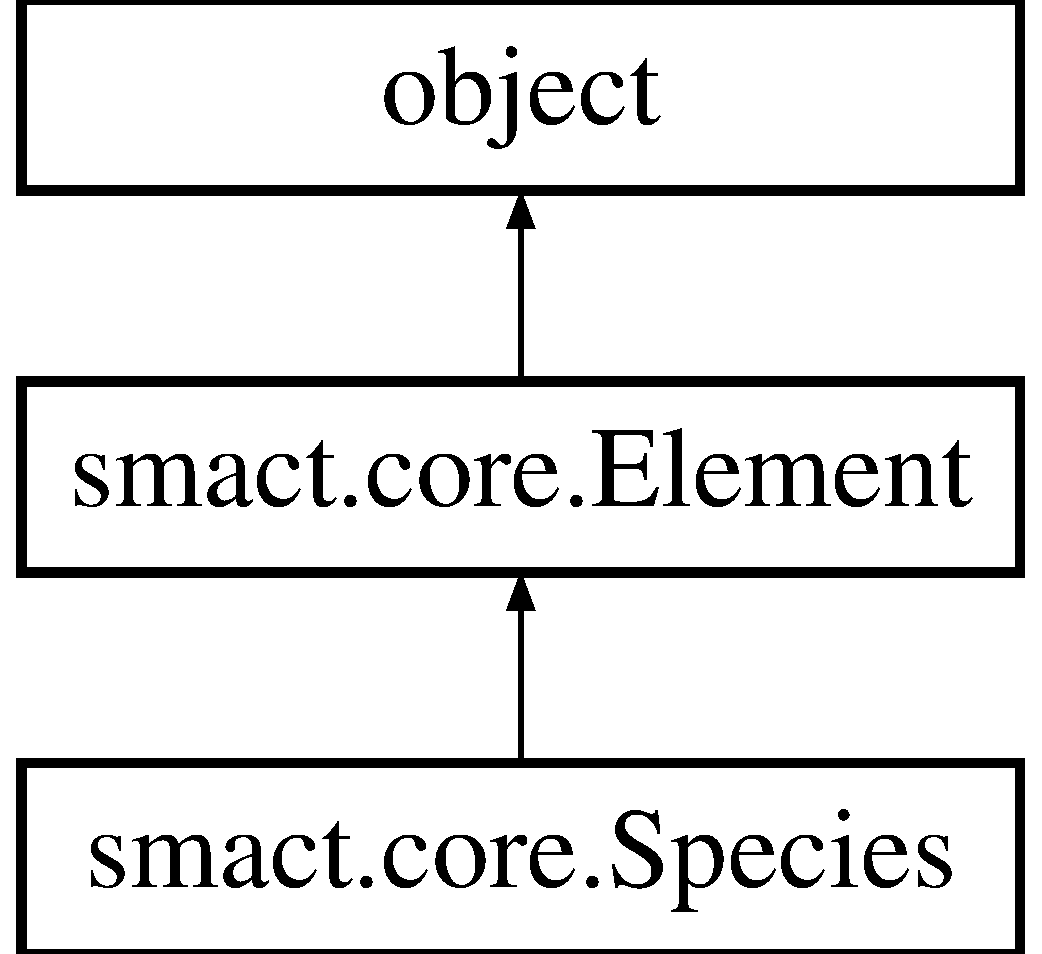
\includegraphics[height=3.000000cm]{classsmact_1_1core_1_1_element}
\end{center}
\end{figure}
\subsection*{Public Member Functions}
\begin{DoxyCompactItemize}
\item 
def \hyperlink{classsmact_1_1core_1_1_element_a584b465cd6f0c624f5c092f7517d4305}{\+\_\+\+\_\+init\+\_\+\+\_\+}
\end{DoxyCompactItemize}
\subsection*{Public Attributes}
\begin{DoxyCompactItemize}
\item 
\hyperlink{classsmact_1_1core_1_1_element_a48bcda32c64f4b012bb81d5e52b065eb}{oxidation\+\_\+states}
\item 
\hyperlink{classsmact_1_1core_1_1_element_a6a1fb78c04a5d4c60dec746d7a7dd40d}{crustal\+\_\+abundance}
\item 
\hyperlink{classsmact_1_1core_1_1_element_a5f031a6efa10491fd6380613462d96a3}{H\+H\+I\+\_\+p}
\item 
\hyperlink{classsmact_1_1core_1_1_element_a197c7ae8d71c349431538d4458c0c1d7}{H\+H\+I\+\_\+\+R}
\item 
\hyperlink{classsmact_1_1core_1_1_element_a6d08136e1d0c72c81fc84819df2dd445}{symbol}
\item 
\hyperlink{classsmact_1_1core_1_1_element_a89e5ff959b6f096dc9285694d5ab22bd}{name}
\item 
\hyperlink{classsmact_1_1core_1_1_element_a4504f14ceab60eab6bb661a10a9314a5}{number}
\item 
\hyperlink{classsmact_1_1core_1_1_element_a9df0fe14367b21ea290b4b1176161aaf}{covalent\+\_\+radius}
\item 
\hyperlink{classsmact_1_1core_1_1_element_a9d9694ce9663754858c0f8218251628e}{pauling\+\_\+eneg}
\item 
\hyperlink{classsmact_1_1core_1_1_element_ae2ae96c550dc0eec1cb5d9a382ac234f}{ionpot}
\item 
\hyperlink{classsmact_1_1core_1_1_element_af43f90f8073aa781d8b9ba78668aa555}{e\+\_\+affinity}
\item 
\hyperlink{classsmact_1_1core_1_1_element_aa91683b81bb28c62f822b730902fe143}{eig}
\item 
\hyperlink{classsmact_1_1core_1_1_element_a44f7d5b4878a683b060ae821f55a48e8}{eig\+\_\+s}
\item 
\hyperlink{classsmact_1_1core_1_1_element_af8f4048bac5979e89864cdfdade6db76}{coord\+\_\+envs}
\end{DoxyCompactItemize}


\subsection{Detailed Description}
\begin{DoxyVerb}Class providing standard chemical data for elements.\end{DoxyVerb}
 

\subsection{Constructor \& Destructor Documentation}
\hypertarget{classsmact_1_1core_1_1_element_a584b465cd6f0c624f5c092f7517d4305}{}\index{smact\+::core\+::\+Element@{smact\+::core\+::\+Element}!\+\_\+\+\_\+init\+\_\+\+\_\+@{\+\_\+\+\_\+init\+\_\+\+\_\+}}
\index{\+\_\+\+\_\+init\+\_\+\+\_\+@{\+\_\+\+\_\+init\+\_\+\+\_\+}!smact\+::core\+::\+Element@{smact\+::core\+::\+Element}}
\subsubsection[{\+\_\+\+\_\+init\+\_\+\+\_\+}]{\setlength{\rightskip}{0pt plus 5cm}def smact.\+core.\+Element.\+\_\+\+\_\+init\+\_\+\+\_\+ (
\begin{DoxyParamCaption}
\item[{}]{self, }
\item[{}]{symbol}
\end{DoxyParamCaption}
)}\label{classsmact_1_1core_1_1_element_a584b465cd6f0c624f5c092f7517d4305}
\begin{DoxyVerb}Collection of standard elemental properties for given element.
Data is drawn from "data/element.txt", part of the Open Babel package.
element = element('Symbol')

Atoms with a defined oxidation state draw properties from the "Species" class.

Attributes:

    Element.symbol: Elemental symbol used to retrieve data

    Element.name: Full name of element

    Element.number: Proton number of element

    Element.pauling_eneg: Pauling electronegativity (0.0 if unknown)

    Element.ionpot: Ionisation potential in eV (0.0 if unknown)

    Element.e_affinity: Electron affinity in eV (0.0 if unknown)

    Element.eig: Electron eigenvalue (units unknown)
    N.B. For Cu, Au and Ag this defaults to d-orbital.
    TODO(DD): implement a way to select the desired orbital
    
    Element.crustal_abundance: crustal abundance in the earths crust mg/kg taken from CRC
    
    Element.coord_envs: The allowed coordination enviroments for the ion.

Raises:
    NameError: Element not found in element.txt
    Warning: Element not found in Eigenvalues.csv\end{DoxyVerb}
 

\subsection{Member Data Documentation}
\hypertarget{classsmact_1_1core_1_1_element_af8f4048bac5979e89864cdfdade6db76}{}\index{smact\+::core\+::\+Element@{smact\+::core\+::\+Element}!coord\+\_\+envs@{coord\+\_\+envs}}
\index{coord\+\_\+envs@{coord\+\_\+envs}!smact\+::core\+::\+Element@{smact\+::core\+::\+Element}}
\subsubsection[{coord\+\_\+envs}]{\setlength{\rightskip}{0pt plus 5cm}smact.\+core.\+Element.\+coord\+\_\+envs}\label{classsmact_1_1core_1_1_element_af8f4048bac5979e89864cdfdade6db76}
\hypertarget{classsmact_1_1core_1_1_element_a9df0fe14367b21ea290b4b1176161aaf}{}\index{smact\+::core\+::\+Element@{smact\+::core\+::\+Element}!covalent\+\_\+radius@{covalent\+\_\+radius}}
\index{covalent\+\_\+radius@{covalent\+\_\+radius}!smact\+::core\+::\+Element@{smact\+::core\+::\+Element}}
\subsubsection[{covalent\+\_\+radius}]{\setlength{\rightskip}{0pt plus 5cm}smact.\+core.\+Element.\+covalent\+\_\+radius}\label{classsmact_1_1core_1_1_element_a9df0fe14367b21ea290b4b1176161aaf}
\hypertarget{classsmact_1_1core_1_1_element_a6a1fb78c04a5d4c60dec746d7a7dd40d}{}\index{smact\+::core\+::\+Element@{smact\+::core\+::\+Element}!crustal\+\_\+abundance@{crustal\+\_\+abundance}}
\index{crustal\+\_\+abundance@{crustal\+\_\+abundance}!smact\+::core\+::\+Element@{smact\+::core\+::\+Element}}
\subsubsection[{crustal\+\_\+abundance}]{\setlength{\rightskip}{0pt plus 5cm}smact.\+core.\+Element.\+crustal\+\_\+abundance}\label{classsmact_1_1core_1_1_element_a6a1fb78c04a5d4c60dec746d7a7dd40d}
\hypertarget{classsmact_1_1core_1_1_element_af43f90f8073aa781d8b9ba78668aa555}{}\index{smact\+::core\+::\+Element@{smact\+::core\+::\+Element}!e\+\_\+affinity@{e\+\_\+affinity}}
\index{e\+\_\+affinity@{e\+\_\+affinity}!smact\+::core\+::\+Element@{smact\+::core\+::\+Element}}
\subsubsection[{e\+\_\+affinity}]{\setlength{\rightskip}{0pt plus 5cm}smact.\+core.\+Element.\+e\+\_\+affinity}\label{classsmact_1_1core_1_1_element_af43f90f8073aa781d8b9ba78668aa555}
\hypertarget{classsmact_1_1core_1_1_element_aa91683b81bb28c62f822b730902fe143}{}\index{smact\+::core\+::\+Element@{smact\+::core\+::\+Element}!eig@{eig}}
\index{eig@{eig}!smact\+::core\+::\+Element@{smact\+::core\+::\+Element}}
\subsubsection[{eig}]{\setlength{\rightskip}{0pt plus 5cm}smact.\+core.\+Element.\+eig}\label{classsmact_1_1core_1_1_element_aa91683b81bb28c62f822b730902fe143}
\hypertarget{classsmact_1_1core_1_1_element_a44f7d5b4878a683b060ae821f55a48e8}{}\index{smact\+::core\+::\+Element@{smact\+::core\+::\+Element}!eig\+\_\+s@{eig\+\_\+s}}
\index{eig\+\_\+s@{eig\+\_\+s}!smact\+::core\+::\+Element@{smact\+::core\+::\+Element}}
\subsubsection[{eig\+\_\+s}]{\setlength{\rightskip}{0pt plus 5cm}smact.\+core.\+Element.\+eig\+\_\+s}\label{classsmact_1_1core_1_1_element_a44f7d5b4878a683b060ae821f55a48e8}
\hypertarget{classsmact_1_1core_1_1_element_a5f031a6efa10491fd6380613462d96a3}{}\index{smact\+::core\+::\+Element@{smact\+::core\+::\+Element}!H\+H\+I\+\_\+p@{H\+H\+I\+\_\+p}}
\index{H\+H\+I\+\_\+p@{H\+H\+I\+\_\+p}!smact\+::core\+::\+Element@{smact\+::core\+::\+Element}}
\subsubsection[{H\+H\+I\+\_\+p}]{\setlength{\rightskip}{0pt plus 5cm}smact.\+core.\+Element.\+H\+H\+I\+\_\+p}\label{classsmact_1_1core_1_1_element_a5f031a6efa10491fd6380613462d96a3}
\hypertarget{classsmact_1_1core_1_1_element_a197c7ae8d71c349431538d4458c0c1d7}{}\index{smact\+::core\+::\+Element@{smact\+::core\+::\+Element}!H\+H\+I\+\_\+\+R@{H\+H\+I\+\_\+\+R}}
\index{H\+H\+I\+\_\+\+R@{H\+H\+I\+\_\+\+R}!smact\+::core\+::\+Element@{smact\+::core\+::\+Element}}
\subsubsection[{H\+H\+I\+\_\+\+R}]{\setlength{\rightskip}{0pt plus 5cm}smact.\+core.\+Element.\+H\+H\+I\+\_\+\+R}\label{classsmact_1_1core_1_1_element_a197c7ae8d71c349431538d4458c0c1d7}
\hypertarget{classsmact_1_1core_1_1_element_ae2ae96c550dc0eec1cb5d9a382ac234f}{}\index{smact\+::core\+::\+Element@{smact\+::core\+::\+Element}!ionpot@{ionpot}}
\index{ionpot@{ionpot}!smact\+::core\+::\+Element@{smact\+::core\+::\+Element}}
\subsubsection[{ionpot}]{\setlength{\rightskip}{0pt plus 5cm}smact.\+core.\+Element.\+ionpot}\label{classsmact_1_1core_1_1_element_ae2ae96c550dc0eec1cb5d9a382ac234f}
\hypertarget{classsmact_1_1core_1_1_element_a89e5ff959b6f096dc9285694d5ab22bd}{}\index{smact\+::core\+::\+Element@{smact\+::core\+::\+Element}!name@{name}}
\index{name@{name}!smact\+::core\+::\+Element@{smact\+::core\+::\+Element}}
\subsubsection[{name}]{\setlength{\rightskip}{0pt plus 5cm}smact.\+core.\+Element.\+name}\label{classsmact_1_1core_1_1_element_a89e5ff959b6f096dc9285694d5ab22bd}
\hypertarget{classsmact_1_1core_1_1_element_a4504f14ceab60eab6bb661a10a9314a5}{}\index{smact\+::core\+::\+Element@{smact\+::core\+::\+Element}!number@{number}}
\index{number@{number}!smact\+::core\+::\+Element@{smact\+::core\+::\+Element}}
\subsubsection[{number}]{\setlength{\rightskip}{0pt plus 5cm}smact.\+core.\+Element.\+number}\label{classsmact_1_1core_1_1_element_a4504f14ceab60eab6bb661a10a9314a5}
\hypertarget{classsmact_1_1core_1_1_element_a48bcda32c64f4b012bb81d5e52b065eb}{}\index{smact\+::core\+::\+Element@{smact\+::core\+::\+Element}!oxidation\+\_\+states@{oxidation\+\_\+states}}
\index{oxidation\+\_\+states@{oxidation\+\_\+states}!smact\+::core\+::\+Element@{smact\+::core\+::\+Element}}
\subsubsection[{oxidation\+\_\+states}]{\setlength{\rightskip}{0pt plus 5cm}smact.\+core.\+Element.\+oxidation\+\_\+states}\label{classsmact_1_1core_1_1_element_a48bcda32c64f4b012bb81d5e52b065eb}
\hypertarget{classsmact_1_1core_1_1_element_a9d9694ce9663754858c0f8218251628e}{}\index{smact\+::core\+::\+Element@{smact\+::core\+::\+Element}!pauling\+\_\+eneg@{pauling\+\_\+eneg}}
\index{pauling\+\_\+eneg@{pauling\+\_\+eneg}!smact\+::core\+::\+Element@{smact\+::core\+::\+Element}}
\subsubsection[{pauling\+\_\+eneg}]{\setlength{\rightskip}{0pt plus 5cm}smact.\+core.\+Element.\+pauling\+\_\+eneg}\label{classsmact_1_1core_1_1_element_a9d9694ce9663754858c0f8218251628e}
\hypertarget{classsmact_1_1core_1_1_element_a6d08136e1d0c72c81fc84819df2dd445}{}\index{smact\+::core\+::\+Element@{smact\+::core\+::\+Element}!symbol@{symbol}}
\index{symbol@{symbol}!smact\+::core\+::\+Element@{smact\+::core\+::\+Element}}
\subsubsection[{symbol}]{\setlength{\rightskip}{0pt plus 5cm}smact.\+core.\+Element.\+symbol}\label{classsmact_1_1core_1_1_element_a6d08136e1d0c72c81fc84819df2dd445}


The documentation for this class was generated from the following file\+:\begin{DoxyCompactItemize}
\item 
/\+Users/\+K\+T\+B22/\+Source\+Tree/smact/smact/\hyperlink{core_8py}{core.\+py}\end{DoxyCompactItemize}

\hypertarget{classsmact_1_1lattice_1_1_lattice}{}\section{smact.\+lattice.\+Lattice Class Reference}
\label{classsmact_1_1lattice_1_1_lattice}\index{smact.\+lattice.\+Lattice@{smact.\+lattice.\+Lattice}}
Inheritance diagram for smact.\+lattice.\+Lattice\+:\begin{figure}[H]
\begin{center}
\leavevmode
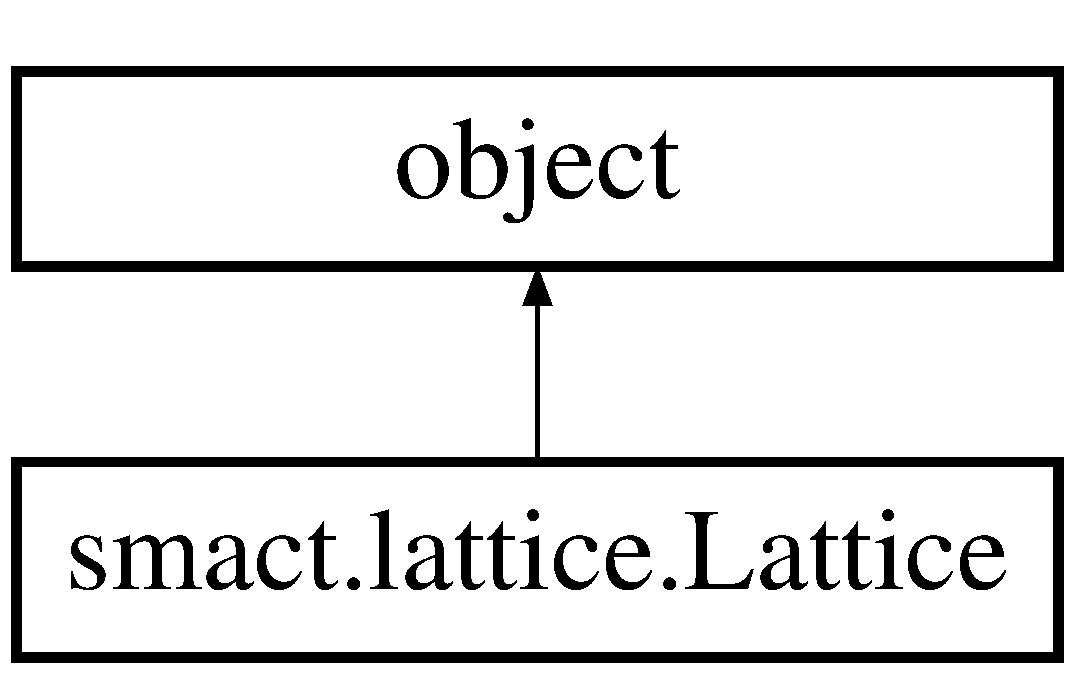
\includegraphics[height=2.000000cm]{classsmact_1_1lattice_1_1_lattice}
\end{center}
\end{figure}
\subsection*{Public Member Functions}
\begin{DoxyCompactItemize}
\item 
def \hyperlink{classsmact_1_1lattice_1_1_lattice_ae825975e73ce79c8f887136a3312539f}{\+\_\+\+\_\+init\+\_\+\+\_\+}
\end{DoxyCompactItemize}
\subsection*{Public Attributes}
\begin{DoxyCompactItemize}
\item 
\hyperlink{classsmact_1_1lattice_1_1_lattice_aebb6987b958080b9cb3a5522733371ea}{sites}
\item 
\hyperlink{classsmact_1_1lattice_1_1_lattice_adc28d116ff0ff923afbd89bd71ca1f3b}{space\+\_\+group}
\item 
\hyperlink{classsmact_1_1lattice_1_1_lattice_a74402107431fd73d860a299bb4a750ce}{strukturbericht}
\end{DoxyCompactItemize}


\subsection{Detailed Description}
\begin{DoxyVerb}A unique set of Sites

Lattice objects define a general crystal structure, with a space group and
a collection of Site objects. These Site objects have their own fractional
coordinates and a list of possible oxidation states (see the Site class).

Specific crystal structures with elements assigned to sites are
"materials" and use the Atoms class from the Atomic Simulation
Environment.

Attributes: 
    basis_sites: A list of Site objects [SiteA, SiteB, SiteC, ...]
    comprising the basis sites in Cartesian coordinates

    space_group: Integer space group number according to the
    International Tables for Crystallography.  

    structurbericht:
    Structurbericht identity, if applicable (e.g. 'B1')

Methods:
    lattice_vector_calc():\end{DoxyVerb}
 

\subsection{Constructor \& Destructor Documentation}
\hypertarget{classsmact_1_1lattice_1_1_lattice_ae825975e73ce79c8f887136a3312539f}{}\index{smact\+::lattice\+::\+Lattice@{smact\+::lattice\+::\+Lattice}!\+\_\+\+\_\+init\+\_\+\+\_\+@{\+\_\+\+\_\+init\+\_\+\+\_\+}}
\index{\+\_\+\+\_\+init\+\_\+\+\_\+@{\+\_\+\+\_\+init\+\_\+\+\_\+}!smact\+::lattice\+::\+Lattice@{smact\+::lattice\+::\+Lattice}}
\subsubsection[{\+\_\+\+\_\+init\+\_\+\+\_\+}]{\setlength{\rightskip}{0pt plus 5cm}def smact.\+lattice.\+Lattice.\+\_\+\+\_\+init\+\_\+\+\_\+ (
\begin{DoxyParamCaption}
\item[{}]{self, }
\item[{}]{sites, }
\item[{}]{space\+\_\+group = {\ttfamily 1}, }
\item[{}]{strukturbericht = {\ttfamily False}}
\end{DoxyParamCaption}
)}\label{classsmact_1_1lattice_1_1_lattice_ae825975e73ce79c8f887136a3312539f}


\subsection{Member Data Documentation}
\hypertarget{classsmact_1_1lattice_1_1_lattice_aebb6987b958080b9cb3a5522733371ea}{}\index{smact\+::lattice\+::\+Lattice@{smact\+::lattice\+::\+Lattice}!sites@{sites}}
\index{sites@{sites}!smact\+::lattice\+::\+Lattice@{smact\+::lattice\+::\+Lattice}}
\subsubsection[{sites}]{\setlength{\rightskip}{0pt plus 5cm}smact.\+lattice.\+Lattice.\+sites}\label{classsmact_1_1lattice_1_1_lattice_aebb6987b958080b9cb3a5522733371ea}
\hypertarget{classsmact_1_1lattice_1_1_lattice_adc28d116ff0ff923afbd89bd71ca1f3b}{}\index{smact\+::lattice\+::\+Lattice@{smact\+::lattice\+::\+Lattice}!space\+\_\+group@{space\+\_\+group}}
\index{space\+\_\+group@{space\+\_\+group}!smact\+::lattice\+::\+Lattice@{smact\+::lattice\+::\+Lattice}}
\subsubsection[{space\+\_\+group}]{\setlength{\rightskip}{0pt plus 5cm}smact.\+lattice.\+Lattice.\+space\+\_\+group}\label{classsmact_1_1lattice_1_1_lattice_adc28d116ff0ff923afbd89bd71ca1f3b}
\hypertarget{classsmact_1_1lattice_1_1_lattice_a74402107431fd73d860a299bb4a750ce}{}\index{smact\+::lattice\+::\+Lattice@{smact\+::lattice\+::\+Lattice}!strukturbericht@{strukturbericht}}
\index{strukturbericht@{strukturbericht}!smact\+::lattice\+::\+Lattice@{smact\+::lattice\+::\+Lattice}}
\subsubsection[{strukturbericht}]{\setlength{\rightskip}{0pt plus 5cm}smact.\+lattice.\+Lattice.\+strukturbericht}\label{classsmact_1_1lattice_1_1_lattice_a74402107431fd73d860a299bb4a750ce}


The documentation for this class was generated from the following file\+:\begin{DoxyCompactItemize}
\item 
/\+Users/\+K\+T\+B22/\+Source\+Tree/smact/smact/\hyperlink{lattice_8py}{lattice.\+py}\end{DoxyCompactItemize}

\hypertarget{classsmact_1_1lattice_1_1_site}{}\section{smact.\+lattice.\+Site Class Reference}
\label{classsmact_1_1lattice_1_1_site}\index{smact.\+lattice.\+Site@{smact.\+lattice.\+Site}}
Inheritance diagram for smact.\+lattice.\+Site\+:\begin{figure}[H]
\begin{center}
\leavevmode
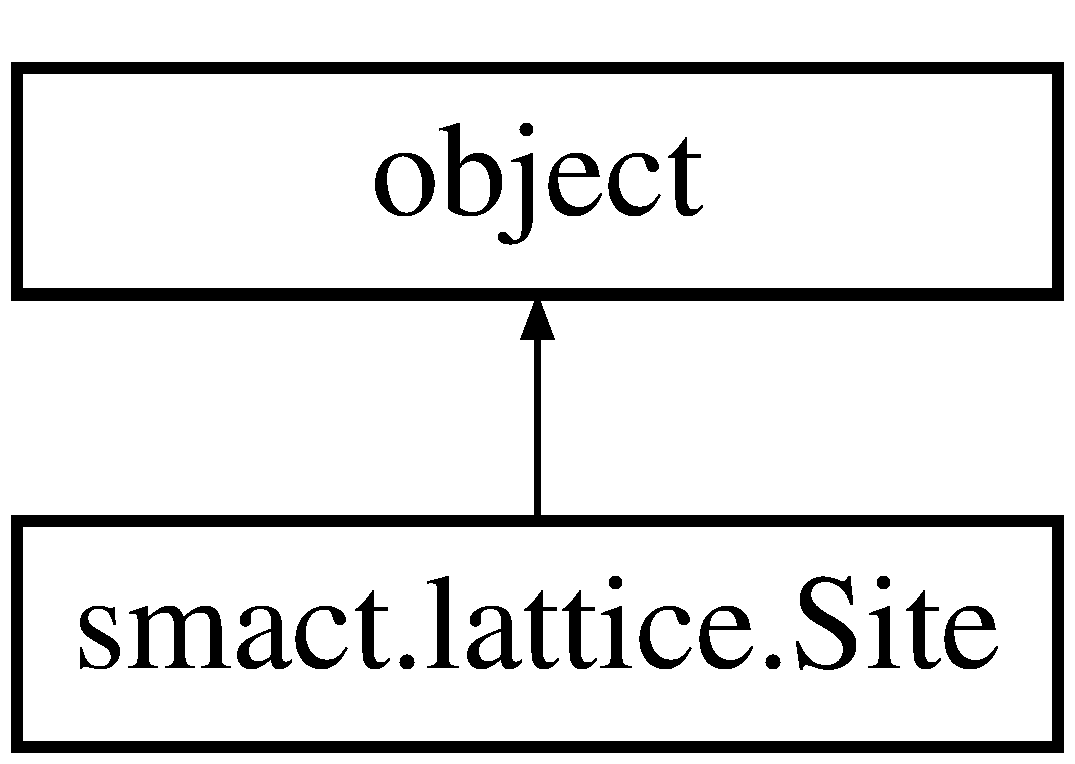
\includegraphics[height=2.000000cm]{classsmact_1_1lattice_1_1_site}
\end{center}
\end{figure}
\subsection*{Public Member Functions}
\begin{DoxyCompactItemize}
\item 
def \hyperlink{classsmact_1_1lattice_1_1_site_a0c838c2b11ae9e20000de848c32a54fd}{\+\_\+\+\_\+init\+\_\+\+\_\+}
\end{DoxyCompactItemize}
\subsection*{Public Attributes}
\begin{DoxyCompactItemize}
\item 
\hyperlink{classsmact_1_1lattice_1_1_site_a5efb051f6bc1d551ad5f68417158fba7}{position}
\item 
\hyperlink{classsmact_1_1lattice_1_1_site_afd3f05ccf43e4f9199033787f0969fcd}{oxidation\+\_\+states}
\end{DoxyCompactItemize}


\subsection{Detailed Description}
\begin{DoxyVerb}A single lattice site with a list of possible oxidation states

The Site object is primarily used within Lattice objects.

Attributes:
    position: A list of fractional coordinates [x,y,z]
    oxidation_states: A list of possible oxidation states e.g. [-1,0,1]\end{DoxyVerb}
 

\subsection{Constructor \& Destructor Documentation}
\hypertarget{classsmact_1_1lattice_1_1_site_a0c838c2b11ae9e20000de848c32a54fd}{}\index{smact\+::lattice\+::\+Site@{smact\+::lattice\+::\+Site}!\+\_\+\+\_\+init\+\_\+\+\_\+@{\+\_\+\+\_\+init\+\_\+\+\_\+}}
\index{\+\_\+\+\_\+init\+\_\+\+\_\+@{\+\_\+\+\_\+init\+\_\+\+\_\+}!smact\+::lattice\+::\+Site@{smact\+::lattice\+::\+Site}}
\subsubsection[{\+\_\+\+\_\+init\+\_\+\+\_\+}]{\setlength{\rightskip}{0pt plus 5cm}def smact.\+lattice.\+Site.\+\_\+\+\_\+init\+\_\+\+\_\+ (
\begin{DoxyParamCaption}
\item[{}]{self, }
\item[{}]{position, }
\item[{}]{oxidation\+\_\+states = {\ttfamily \mbox{[}0\mbox{]}}}
\end{DoxyParamCaption}
)}\label{classsmact_1_1lattice_1_1_site_a0c838c2b11ae9e20000de848c32a54fd}


\subsection{Member Data Documentation}
\hypertarget{classsmact_1_1lattice_1_1_site_afd3f05ccf43e4f9199033787f0969fcd}{}\index{smact\+::lattice\+::\+Site@{smact\+::lattice\+::\+Site}!oxidation\+\_\+states@{oxidation\+\_\+states}}
\index{oxidation\+\_\+states@{oxidation\+\_\+states}!smact\+::lattice\+::\+Site@{smact\+::lattice\+::\+Site}}
\subsubsection[{oxidation\+\_\+states}]{\setlength{\rightskip}{0pt plus 5cm}smact.\+lattice.\+Site.\+oxidation\+\_\+states}\label{classsmact_1_1lattice_1_1_site_afd3f05ccf43e4f9199033787f0969fcd}
\hypertarget{classsmact_1_1lattice_1_1_site_a5efb051f6bc1d551ad5f68417158fba7}{}\index{smact\+::lattice\+::\+Site@{smact\+::lattice\+::\+Site}!position@{position}}
\index{position@{position}!smact\+::lattice\+::\+Site@{smact\+::lattice\+::\+Site}}
\subsubsection[{position}]{\setlength{\rightskip}{0pt plus 5cm}smact.\+lattice.\+Site.\+position}\label{classsmact_1_1lattice_1_1_site_a5efb051f6bc1d551ad5f68417158fba7}


The documentation for this class was generated from the following file\+:\begin{DoxyCompactItemize}
\item 
/\+Users/\+K\+T\+B22/\+Source\+Tree/smact/smact/\hyperlink{lattice_8py}{lattice.\+py}\end{DoxyCompactItemize}

\hypertarget{classsmact_1_1core_1_1_species}{}\section{smact.\+core.\+Species Class Reference}
\label{classsmact_1_1core_1_1_species}\index{smact.\+core.\+Species@{smact.\+core.\+Species}}
Inheritance diagram for smact.\+core.\+Species\+:\begin{figure}[H]
\begin{center}
\leavevmode
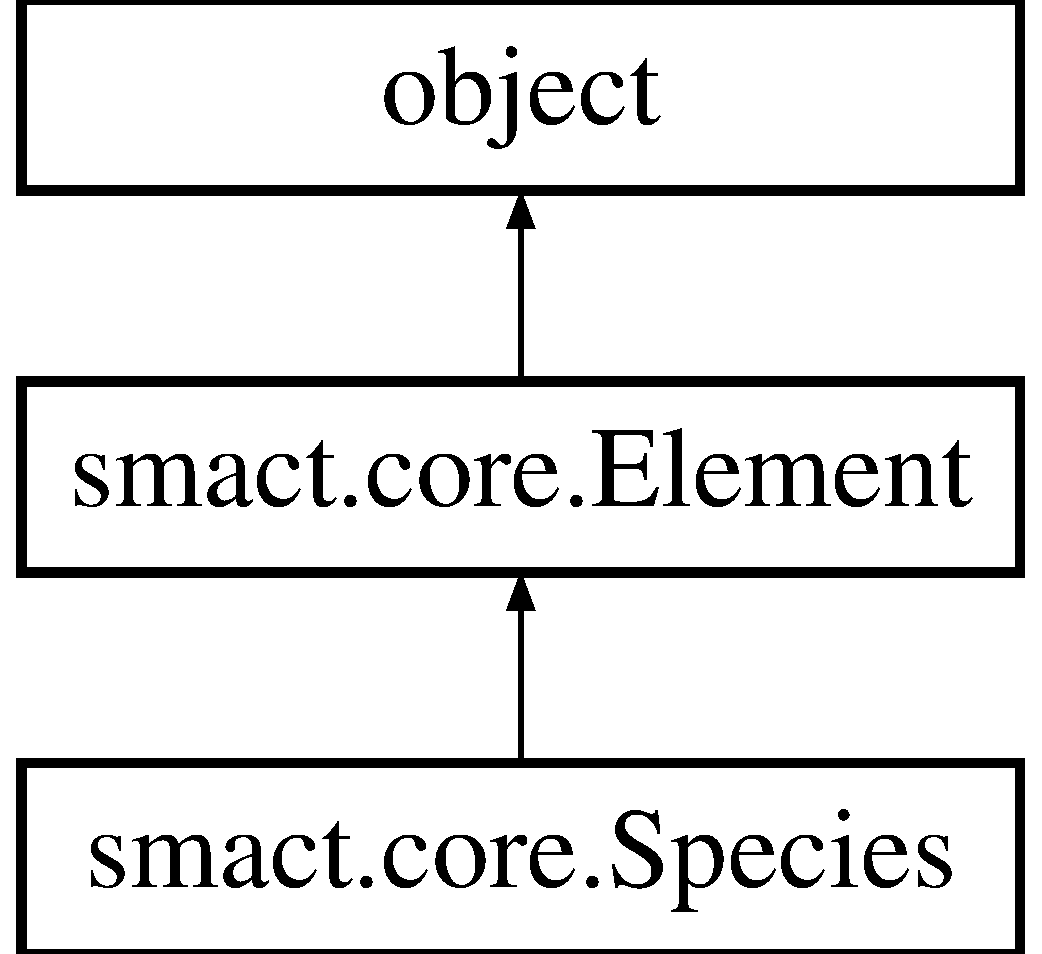
\includegraphics[height=3.000000cm]{classsmact_1_1core_1_1_species}
\end{center}
\end{figure}
\subsection*{Public Member Functions}
\begin{DoxyCompactItemize}
\item 
def \hyperlink{classsmact_1_1core_1_1_species_a186239ed056e1ff2a5c26c29d2fd87ff}{\+\_\+\+\_\+init\+\_\+\+\_\+}
\end{DoxyCompactItemize}
\subsection*{Public Attributes}
\begin{DoxyCompactItemize}
\item 
\hyperlink{classsmact_1_1core_1_1_species_aa7e923db8eba011ccd5cbf7da36707ec}{oxidation}
\item 
\hyperlink{classsmact_1_1core_1_1_species_a4e9691114a02162516af95d4974f1541}{coordination}
\item 
\hyperlink{classsmact_1_1core_1_1_species_a4b07462f361429921475d57e057cdd2b}{shannon\+\_\+radius}
\end{DoxyCompactItemize}


\subsection{Detailed Description}
\begin{DoxyVerb}Class providing data for elements in a given chemical environment

In addition to the standard properties from the periodic table (inherited from the 
Element class), Species objects use the oxidation state and coordination environment
to provide further properties.

Attributes: 
    Species.symbol: Elemental symbol used to retrieve data

    Species.name: Full name of element

    Species.oxidation: Oxidation state of species (signed integer)

    Species.coordination: Coordination number of species (integer)

    Species.pauling_eneg: Pauling electronegativity (0.0 if unknown)

    Species.ionpot: Ionisation potential in eV (0.0 if unknown)

    Species.e_affinity: Electron affinity in eV (0.0 if unknown)

    Species.eig: Electron eigenvalue (units unknown)
    N.B. For Cu, Au and Ag this defaults to d-orbital.
    TODO(DD): implement a way to select the desired orbital

Raises:
    NameError: Element not found in element.txt
    Warning: Element not found in Eigenvalues.csv              \end{DoxyVerb}
 

\subsection{Constructor \& Destructor Documentation}
\hypertarget{classsmact_1_1core_1_1_species_a186239ed056e1ff2a5c26c29d2fd87ff}{}\index{smact\+::core\+::\+Species@{smact\+::core\+::\+Species}!\+\_\+\+\_\+init\+\_\+\+\_\+@{\+\_\+\+\_\+init\+\_\+\+\_\+}}
\index{\+\_\+\+\_\+init\+\_\+\+\_\+@{\+\_\+\+\_\+init\+\_\+\+\_\+}!smact\+::core\+::\+Species@{smact\+::core\+::\+Species}}
\subsubsection[{\+\_\+\+\_\+init\+\_\+\+\_\+}]{\setlength{\rightskip}{0pt plus 5cm}def smact.\+core.\+Species.\+\_\+\+\_\+init\+\_\+\+\_\+ (
\begin{DoxyParamCaption}
\item[{}]{self, }
\item[{}]{symbol, }
\item[{}]{oxidation, }
\item[{}]{coordination}
\end{DoxyParamCaption}
)}\label{classsmact_1_1core_1_1_species_a186239ed056e1ff2a5c26c29d2fd87ff}


\subsection{Member Data Documentation}
\hypertarget{classsmact_1_1core_1_1_species_a4e9691114a02162516af95d4974f1541}{}\index{smact\+::core\+::\+Species@{smact\+::core\+::\+Species}!coordination@{coordination}}
\index{coordination@{coordination}!smact\+::core\+::\+Species@{smact\+::core\+::\+Species}}
\subsubsection[{coordination}]{\setlength{\rightskip}{0pt plus 5cm}smact.\+core.\+Species.\+coordination}\label{classsmact_1_1core_1_1_species_a4e9691114a02162516af95d4974f1541}
\hypertarget{classsmact_1_1core_1_1_species_aa7e923db8eba011ccd5cbf7da36707ec}{}\index{smact\+::core\+::\+Species@{smact\+::core\+::\+Species}!oxidation@{oxidation}}
\index{oxidation@{oxidation}!smact\+::core\+::\+Species@{smact\+::core\+::\+Species}}
\subsubsection[{oxidation}]{\setlength{\rightskip}{0pt plus 5cm}smact.\+core.\+Species.\+oxidation}\label{classsmact_1_1core_1_1_species_aa7e923db8eba011ccd5cbf7da36707ec}
\hypertarget{classsmact_1_1core_1_1_species_a4b07462f361429921475d57e057cdd2b}{}\index{smact\+::core\+::\+Species@{smact\+::core\+::\+Species}!shannon\+\_\+radius@{shannon\+\_\+radius}}
\index{shannon\+\_\+radius@{shannon\+\_\+radius}!smact\+::core\+::\+Species@{smact\+::core\+::\+Species}}
\subsubsection[{shannon\+\_\+radius}]{\setlength{\rightskip}{0pt plus 5cm}smact.\+core.\+Species.\+shannon\+\_\+radius}\label{classsmact_1_1core_1_1_species_a4b07462f361429921475d57e057cdd2b}


The documentation for this class was generated from the following file\+:\begin{DoxyCompactItemize}
\item 
/\+Users/\+K\+T\+B22/\+Source\+Tree/smact/smact/\hyperlink{core_8py}{core.\+py}\end{DoxyCompactItemize}

\chapter{File Documentation}
\hypertarget{____init_____8py}{}\section{/\+Users/\+K\+T\+B22/\+Source\+Tree/smact/smact/\+\_\+\+\_\+init\+\_\+\+\_\+.py File Reference}
\label{____init_____8py}\index{/\+Users/\+K\+T\+B22/\+Source\+Tree/smact/smact/\+\_\+\+\_\+init\+\_\+\+\_\+.\+py@{/\+Users/\+K\+T\+B22/\+Source\+Tree/smact/smact/\+\_\+\+\_\+init\+\_\+\+\_\+.\+py}}
\subsection*{Namespaces}
\begin{DoxyCompactItemize}
\item 
 \hyperlink{namespacesmact}{smact}
\end{DoxyCompactItemize}

\hypertarget{properties_2____init_____8py}{}\section{/\+Users/\+K\+T\+B22/\+Source\+Tree/smact/smact/properties/\+\_\+\+\_\+init\+\_\+\+\_\+.py File Reference}
\label{properties_2____init_____8py}\index{/\+Users/\+K\+T\+B22/\+Source\+Tree/smact/smact/properties/\+\_\+\+\_\+init\+\_\+\+\_\+.\+py@{/\+Users/\+K\+T\+B22/\+Source\+Tree/smact/smact/properties/\+\_\+\+\_\+init\+\_\+\+\_\+.\+py}}
\subsection*{Namespaces}
\begin{DoxyCompactItemize}
\item 
 \hyperlink{namespacesmact_1_1properties}{smact.\+properties}
\end{DoxyCompactItemize}

\hypertarget{builder_8py}{}\section{/\+Users/\+K\+T\+B22/\+Source\+Tree/smact/smact/builder.py File Reference}
\label{builder_8py}\index{/\+Users/\+K\+T\+B22/\+Source\+Tree/smact/smact/builder.\+py@{/\+Users/\+K\+T\+B22/\+Source\+Tree/smact/smact/builder.\+py}}
\subsection*{Namespaces}
\begin{DoxyCompactItemize}
\item 
 \hyperlink{namespacesmact_1_1builder}{smact.\+builder}
\end{DoxyCompactItemize}
\subsection*{Functions}
\begin{DoxyCompactItemize}
\item 
def \hyperlink{namespacesmact_1_1builder_a80438d278ab0fd7fc04b82b83f4db074}{smact.\+builder.\+cubic\+\_\+perovskite}
\item 
def \hyperlink{namespacesmact_1_1builder_a3f01529c174cbc12e692be61162bc8d7}{smact.\+builder.\+wurtzite}
\end{DoxyCompactItemize}

\hypertarget{core_8py}{}\section{/\+Users/\+K\+T\+B22/\+Source\+Tree/smact/smact/core.py File Reference}
\label{core_8py}\index{/\+Users/\+K\+T\+B22/\+Source\+Tree/smact/smact/core.\+py@{/\+Users/\+K\+T\+B22/\+Source\+Tree/smact/smact/core.\+py}}
\subsection*{Classes}
\begin{DoxyCompactItemize}
\item 
class \hyperlink{classsmact_1_1core_1_1_element}{smact.\+core.\+Element}
\item 
class \hyperlink{classsmact_1_1core_1_1_species}{smact.\+core.\+Species}
\end{DoxyCompactItemize}
\subsection*{Namespaces}
\begin{DoxyCompactItemize}
\item 
 \hyperlink{namespacesmact_1_1core}{smact.\+core}
\end{DoxyCompactItemize}
\subsection*{Functions}
\begin{DoxyCompactItemize}
\item 
def \hyperlink{namespacesmact_1_1core_a3e8b27f822e17a79e50b1399825564ff}{smact.\+core.\+ordered\+\_\+elements}
\item 
def \hyperlink{namespacesmact_1_1core_a5a32e4b9b50d3db379ede8d7b8b1081a}{smact.\+core.\+are\+\_\+eq}
\item 
def \hyperlink{namespacesmact_1_1core_abd4953dbc9b28e11861b3b63092ec4fa}{smact.\+core.\+lattices\+\_\+are\+\_\+same}
\item 
def \hyperlink{namespacesmact_1_1core_a523386aa44322d0a2670672b4535bab3}{smact.\+core.\+charge\+\_\+neutrality}
\end{DoxyCompactItemize}
\subsection*{Variables}
\begin{DoxyCompactItemize}
\item 
tuple \hyperlink{namespacesmact_1_1core_aaa14f990a82d90eaab5ad3667e72453e}{smact.\+core.\+smact\+\_\+directory} = os.\+path.\+dirname(\+\_\+\+\_\+file\+\_\+\+\_\+)
\end{DoxyCompactItemize}

\hypertarget{data_8py}{}\section{/\+Users/\+K\+T\+B22/\+Source\+Tree/smact/smact/data.py File Reference}
\label{data_8py}\index{/\+Users/\+K\+T\+B22/\+Source\+Tree/smact/smact/data.\+py@{/\+Users/\+K\+T\+B22/\+Source\+Tree/smact/smact/data.\+py}}
\subsection*{Namespaces}
\begin{DoxyCompactItemize}
\item 
 \hyperlink{namespacesmact_1_1data}{smact.\+data}
\end{DoxyCompactItemize}
\subsection*{Functions}
\begin{DoxyCompactItemize}
\item 
def \hyperlink{namespacesmact_1_1data_a2cb4d9dded3d65889eff3badac947922}{smact.\+data.\+get\+\_\+mulliken}
\begin{DoxyCompactList}\small\item\em Copyright Daniel Davies, Adam J. \end{DoxyCompactList}\item 
def \hyperlink{namespacesmact_1_1data_a5777f26050189e84aff07dff82185d05}{smact.\+data.\+get\+\_\+pauling}
\begin{DoxyCompactList}\small\item\em The following functions are deprecated. \end{DoxyCompactList}\item 
def \hyperlink{namespacesmact_1_1data_a99f38b1d5bd7e101330f88fd1aedb794}{smact.\+data.\+get\+\_\+covalent}
\item 
def \hyperlink{namespacesmact_1_1data_af25e690defd2aa1923b815cb5eb73ca6}{smact.\+data.\+get\+\_\+eig}
\item 
def \hyperlink{namespacesmact_1_1data_a80cf4a9c06413608e98a6086dbedb87b}{smact.\+data.\+get\+\_\+eig\+\_\+s}
\item 
def \hyperlink{namespacesmact_1_1data_a5249c4b761aa5c3a2d06dabdac2fafbf}{smact.\+data.\+get\+\_\+ionic}
\end{DoxyCompactItemize}

\hypertarget{distorter_8py}{}\section{/\+Users/\+K\+T\+B22/\+Source\+Tree/smact/smact/distorter.py File Reference}
\label{distorter_8py}\index{/\+Users/\+K\+T\+B22/\+Source\+Tree/smact/smact/distorter.\+py@{/\+Users/\+K\+T\+B22/\+Source\+Tree/smact/smact/distorter.\+py}}
\subsection*{Namespaces}
\begin{DoxyCompactItemize}
\item 
 \hyperlink{namespacesmact_1_1distorter}{smact.\+distorter}
\end{DoxyCompactItemize}
\subsection*{Functions}
\begin{DoxyCompactItemize}
\item 
def \hyperlink{namespacesmact_1_1distorter_a0ac75ed2f6cb305b3c8596d94517eec6}{smact.\+distorter.\+get\+\_\+sg}
\item 
def \hyperlink{namespacesmact_1_1distorter_a1ec14de462a0176842705f8fc4c9c39b}{smact.\+distorter.\+get\+\_\+inequivalent\+\_\+sites}
\item 
def \hyperlink{namespacesmact_1_1distorter_ade340d55f2d7f76740c01bbc79e3be91}{smact.\+distorter.\+make\+\_\+substitution}
\item 
def \hyperlink{namespacesmact_1_1distorter_a39d7cc60d45b249ab88edc3ec929e68b}{smact.\+distorter.\+build\+\_\+sub\+\_\+lattice}
\end{DoxyCompactItemize}

\hypertarget{lattice_8py}{}\section{/\+Users/\+K\+T\+B22/\+Source\+Tree/smact/smact/lattice.py File Reference}
\label{lattice_8py}\index{/\+Users/\+K\+T\+B22/\+Source\+Tree/smact/smact/lattice.\+py@{/\+Users/\+K\+T\+B22/\+Source\+Tree/smact/smact/lattice.\+py}}
\subsection*{Classes}
\begin{DoxyCompactItemize}
\item 
class \hyperlink{classsmact_1_1lattice_1_1_lattice}{smact.\+lattice.\+Lattice}
\item 
class \hyperlink{classsmact_1_1lattice_1_1_site}{smact.\+lattice.\+Site}
\end{DoxyCompactItemize}
\subsection*{Namespaces}
\begin{DoxyCompactItemize}
\item 
 \hyperlink{namespacesmact_1_1lattice}{smact.\+lattice}
\end{DoxyCompactItemize}
\subsection*{Functions}
\begin{DoxyCompactItemize}
\item 
def \hyperlink{namespacesmact_1_1lattice_a0380cf2cee37daa74c90bbefa4a16246}{smact.\+lattice.\+check\+\_\+lattice\+\_\+charges}
\item 
def \hyperlink{namespacesmact_1_1lattice_af33a880afcb916626bc20669a084457f}{smact.\+lattice.\+possible\+\_\+compositions}
\item 
def \hyperlink{namespacesmact_1_1lattice_a480b77e0ed0d4874c376d27f41ee0b3c}{smact.\+lattice.\+possible\+\_\+elements}
\end{DoxyCompactItemize}

\hypertarget{lattice__parameters_8py}{}\section{/\+Users/\+K\+T\+B22/\+Source\+Tree/smact/smact/lattice\+\_\+parameters.py File Reference}
\label{lattice__parameters_8py}\index{/\+Users/\+K\+T\+B22/\+Source\+Tree/smact/smact/lattice\+\_\+parameters.\+py@{/\+Users/\+K\+T\+B22/\+Source\+Tree/smact/smact/lattice\+\_\+parameters.\+py}}
\subsection*{Namespaces}
\begin{DoxyCompactItemize}
\item 
 \hyperlink{namespacesmact_1_1lattice__parameters}{smact.\+lattice\+\_\+parameters}
\end{DoxyCompactItemize}
\subsection*{Functions}
\begin{DoxyCompactItemize}
\item 
def \hyperlink{namespacesmact_1_1lattice__parameters_ad362e3a76b00a5dad0aab8ec370525d4}{smact.\+lattice\+\_\+parameters.\+cubic\+\_\+perovskite}
\item 
def \hyperlink{namespacesmact_1_1lattice__parameters_ad9f584d4e062d087e18aeca194c2537b}{smact.\+lattice\+\_\+parameters.\+wurtzite}
\item 
def \hyperlink{namespacesmact_1_1lattice__parameters_a4e67c0acfd178548e38a8ae341791259}{smact.\+lattice\+\_\+parameters.\+fcc}
\item 
def \hyperlink{namespacesmact_1_1lattice__parameters_a797eec432832ec55c5da86125c120779}{smact.\+lattice\+\_\+parameters.\+bcc}
\item 
def \hyperlink{namespacesmact_1_1lattice__parameters_a09030d3085ef12b8a3d03ce1f1ebc3d0}{smact.\+lattice\+\_\+parameters.\+hcp}
\item 
def \hyperlink{namespacesmact_1_1lattice__parameters_a91b06ba66685101060602b6ce67544f3}{smact.\+lattice\+\_\+parameters.\+diamond}
\item 
def \hyperlink{namespacesmact_1_1lattice__parameters_a26ba203667ced3e22d3a81ec900697a3}{smact.\+lattice\+\_\+parameters.\+bct}
\item 
def \hyperlink{namespacesmact_1_1lattice__parameters_aedc15cf81227b0bbd8fae3e7154b5367}{smact.\+lattice\+\_\+parameters.\+rocksalt}
\item 
def \hyperlink{namespacesmact_1_1lattice__parameters_ae51af656e3f0d10e9a8e12faa3eabfd7}{smact.\+lattice\+\_\+parameters.\+b2}
\item 
def \hyperlink{namespacesmact_1_1lattice__parameters_a4d323fb11b47663e45019e765158e1b1}{smact.\+lattice\+\_\+parameters.\+zincblende}
\item 
def \hyperlink{namespacesmact_1_1lattice__parameters_a632d06c0e2efba1c03f4d42b85792b76}{smact.\+lattice\+\_\+parameters.\+b10}
\begin{DoxyCompactList}\small\item\em Zn-\/\+S-\/\+Zn angle is $\sim$109.5 degrees (from a tetrahedron). \end{DoxyCompactList}\end{DoxyCompactItemize}

\hypertarget{mainpage_8py}{}\section{/\+Users/\+K\+T\+B22/\+Source\+Tree/smact/smact/mainpage.py File Reference}
\label{mainpage_8py}\index{/\+Users/\+K\+T\+B22/\+Source\+Tree/smact/smact/mainpage.\+py@{/\+Users/\+K\+T\+B22/\+Source\+Tree/smact/smact/mainpage.\+py}}
\subsection*{Namespaces}
\begin{DoxyCompactItemize}
\item 
 \hyperlink{namespacesmact_1_1mainpage}{smact.\+mainpage}
\end{DoxyCompactItemize}

\hypertarget{parameters_8py}{}\section{/\+Users/\+K\+T\+B22/\+Source\+Tree/smact/smact/parameters.py File Reference}
\label{parameters_8py}\index{/\+Users/\+K\+T\+B22/\+Source\+Tree/smact/smact/parameters.\+py@{/\+Users/\+K\+T\+B22/\+Source\+Tree/smact/smact/parameters.\+py}}
\subsection*{Namespaces}
\begin{DoxyCompactItemize}
\item 
 \hyperlink{namespacesmact_1_1parameters}{smact.\+parameters}
\end{DoxyCompactItemize}
\subsection*{Functions}
\begin{DoxyCompactItemize}
\item 
def \hyperlink{namespacesmact_1_1parameters_a0a7b9cfac24902170e135aa34e25f674}{smact.\+parameters.\+query\+\_\+yes\+\_\+no}
\item 
def \hyperlink{namespacesmact_1_1parameters_a16867ca20c91dd8b7f4d519b220b08e3}{smact.\+parameters.\+fcc}
\item 
def \hyperlink{namespacesmact_1_1parameters_a1bae56380a1d36c8c0a2fe0323fb1ba5}{smact.\+parameters.\+bcc}
\item 
def \hyperlink{namespacesmact_1_1parameters_a1e720a4abb24a6ab1e663e1ac70b1db1}{smact.\+parameters.\+hcp}
\item 
def \hyperlink{namespacesmact_1_1parameters_a7acfd40bb068480e79670cfe1960f21d}{smact.\+parameters.\+diamond}
\item 
def \hyperlink{namespacesmact_1_1parameters_a16ccefd0b7e9ced870e9bb28cd9caa18}{smact.\+parameters.\+bct}
\item 
def \hyperlink{namespacesmact_1_1parameters_afde267246e2f4aded9e49557939c2a0b}{smact.\+parameters.\+rocksalt}
\item 
def \hyperlink{namespacesmact_1_1parameters_a6517436ba44653f21ddbb58b73b8fb84}{smact.\+parameters.\+b2}
\item 
def \hyperlink{namespacesmact_1_1parameters_a3b2f879f7fa985be9f19a9991addb20e}{smact.\+parameters.\+zincblende}
\item 
def \hyperlink{namespacesmact_1_1parameters_ab26b2a7bf4ad5538de465332c1a7c09b}{smact.\+parameters.\+wurtzite}
\begin{DoxyCompactList}\small\item\em Zn-\/\+S-\/\+Zn angle is $\sim$109.5 degrees (from a tetrahedron). \end{DoxyCompactList}\item 
def \hyperlink{namespacesmact_1_1parameters_afca249beab0792afc200ee2fc1714fbe}{smact.\+parameters.\+b10}
\item 
def \hyperlink{namespacesmact_1_1parameters_a65318bbc38b59562936b20c221a64a22}{smact.\+parameters.\+E2\+\_\+1}
\end{DoxyCompactItemize}
\subsection*{Variables}
\begin{DoxyCompactItemize}
\item 
list \hyperlink{namespacesmact_1_1parameters_afc9fe46cf8520399c024a279a27b8031}{smact.\+parameters.\+a\+\_\+lattices} = \mbox{[}fcc,bcc,hcp,diamond,bct\mbox{]}
\item 
list \hyperlink{namespacesmact_1_1parameters_a998d11eabc47866af083d819a2dca9cf}{smact.\+parameters.\+b\+\_\+lattices} = \mbox{[}rocksalt,b2,zincblende,wurtzite,b10\mbox{]}
\begin{DoxyCompactList}\small\item\em Angle (w) between face-\/centered atom measured to be $\sim$117.8 deg for Sn\+O and Pb\+O, where atoms are not similar in size. \end{DoxyCompactList}\item 
list \hyperlink{namespacesmact_1_1parameters_abdc23b776276418ce7044c62e52c2a32}{smact.\+parameters.\+e\+\_\+lattices} = \mbox{[}E2\+\_\+1\mbox{]}
\item 
tuple \hyperlink{namespacesmact_1_1parameters_a88c84d99ceb967bfb250f0b64c8a7818}{smact.\+parameters.\+crystal\+\_\+elements} = raw\+\_\+input('Which elements? Separate chemical symbols with a space. ')
\item 
\hyperlink{namespacesmact_1_1parameters_a17a85db758a777f49064168e1c8c9d6b}{smact.\+parameters.\+perov} = False
\item 
tuple \hyperlink{namespacesmact_1_1parameters_a7ffa704a6ef8436803e18fcef5d9f65c}{smact.\+parameters.\+x} = core.\+Element(elements)
\begin{DoxyCompactList}\small\item\em A-\/types. \end{DoxyCompactList}\item 
list \hyperlink{namespacesmact_1_1parameters_a14180ce62d67208c70ba3d513c19e6ca}{smact.\+parameters.\+oxidation} = \mbox{[}$\,$\mbox{]}
\item 
list \hyperlink{namespacesmact_1_1parameters_a7823c63853e52a4e3204169fbec5217e}{smact.\+parameters.\+coordination} = \mbox{[}$\,$\mbox{]}
\item 
int \hyperlink{namespacesmact_1_1parameters_a873ca6b8e0241804cc12ff4987d1a102}{smact.\+parameters.\+i} = 0
\item 
list \hyperlink{namespacesmact_1_1parameters_a90bc30a9396fded6e78219dda2380290}{smact.\+parameters.\+poss\+\_\+ox} = \mbox{[}$\,$\mbox{]}
\item 
list \hyperlink{namespacesmact_1_1parameters_a35421c1ebaf66b12a05908c56bc84e23}{smact.\+parameters.\+poss\+\_\+cood} = \mbox{[}$\,$\mbox{]}
\item 
tuple \hyperlink{namespacesmact_1_1parameters_a3fdea3c0c08ebe498efc38f3c3cacb96}{smact.\+parameters.\+reader} = csv.\+reader(f)
\begin{DoxyCompactList}\small\item\em Duplicates removed. \end{DoxyCompactList}\item 
list \hyperlink{namespacesmact_1_1parameters_a871efc9dce945c3476e9b4767745607e}{smact.\+parameters.\+poss\+\_\+ox\+\_\+clean} = \mbox{[}$\,$\mbox{]}
\item 
list \hyperlink{namespacesmact_1_1parameters_a2f0606907d6627c0aa3f575ab28e6f6e}{smact.\+parameters.\+poss\+\_\+co\+\_\+clean} = \mbox{[}$\,$\mbox{]}
\begin{DoxyCompactList}\small\item\em Duplicates removed. \end{DoxyCompactList}\item 
list \hyperlink{namespacesmact_1_1parameters_ac0c38ccc1997b7b2994407fd74c58e5a}{smact.\+parameters.\+shannon\+\_\+radius} = \mbox{[}$\,$\mbox{]}
\begin{DoxyCompactList}\small\item\em B-\/types -\/-\/-\/-\/-\/-\/-\/-\/-\/-\/-\/-\/-\/-\/-\/-\/-\/-\/-\/-\/-\/-\/-\/-\/-\/-\/-\/-\/-\/-\/-\/-\/-\/-\/-\/-\/-\/-\/-\/-\/-\/-\/-\/-\/-\/-\/-\/-\/-\/-\/-\/-\/-\/-\/-\/-\/-\/-\/-\/-\/-\/-\/-\/-\/-\/-\/-\/-\/-\/-\/-\/-\/-\/-\/-\/-\/-\/-\/-\/-\/-\/-\/---\#. \end{DoxyCompactList}\item 
tuple \hyperlink{namespacesmact_1_1parameters_a4ca83f9b909f7195148ffd44a439bd16}{smact.\+parameters.\+inner\+\_\+space} = a$\ast$(6$\ast$$\ast$0.\+5)
\end{DoxyCompactItemize}

\hypertarget{_band__gap__full_8py}{}\section{/\+Users/\+K\+T\+B22/\+Source\+Tree/smact/smact/properties/\+Band\+\_\+gap\+\_\+full.py File Reference}
\label{_band__gap__full_8py}\index{/\+Users/\+K\+T\+B22/\+Source\+Tree/smact/smact/properties/\+Band\+\_\+gap\+\_\+full.\+py@{/\+Users/\+K\+T\+B22/\+Source\+Tree/smact/smact/properties/\+Band\+\_\+gap\+\_\+full.\+py}}
\subsection*{Namespaces}
\begin{DoxyCompactItemize}
\item 
 \hyperlink{namespacesmact_1_1properties_1_1_band__gap__full}{smact.\+properties.\+Band\+\_\+gap\+\_\+full}
\end{DoxyCompactItemize}
\subsection*{Variables}
\begin{DoxyCompactItemize}
\item 
float \hyperlink{namespacesmact_1_1properties_1_1_band__gap__full_a33c6d472118643d5753097ba13eb8c63}{smact.\+properties.\+Band\+\_\+gap\+\_\+full.\+Eta\+\_\+sss} = -\/1.\+40
\item 
float \hyperlink{namespacesmact_1_1properties_1_1_band__gap__full_afec9c51df8f8ae4228ad90d10097981b}{smact.\+properties.\+Band\+\_\+gap\+\_\+full.\+Eta\+\_\+sps} = 1.\+84
\item 
float \hyperlink{namespacesmact_1_1properties_1_1_band__gap__full_acd2104fa7868561e3f2e824c96dff9db}{smact.\+properties.\+Band\+\_\+gap\+\_\+full.\+Eta\+\_\+pps} = 3.\+24
\item 
float \hyperlink{namespacesmact_1_1properties_1_1_band__gap__full_ad8248e3b75f41c62bc132eaf7fd7a332}{smact.\+properties.\+Band\+\_\+gap\+\_\+full.\+Eta\+\_\+ppp} = -\/0.\+81
\item 
float \hyperlink{namespacesmact_1_1properties_1_1_band__gap__full_a4db80d70c7da3674fe2e949c069e41bb}{smact.\+properties.\+Band\+\_\+gap\+\_\+full.\+hbarsq\+\_\+over\+\_\+me} = 7.\+62
\item 
tuple \hyperlink{namespacesmact_1_1properties_1_1_band__gap__full_a07754657208eba604cfe8ee09d738332}{smact.\+properties.\+Band\+\_\+gap\+\_\+full.\+Cat} = raw\+\_\+input(\char`\"{}Enter Cation Symbol\+:\char`\"{})
\item 
tuple \hyperlink{namespacesmact_1_1properties_1_1_band__gap__full_acc697d191f70ba02803a3906c6ec6844}{smact.\+properties.\+Band\+\_\+gap\+\_\+full.\+An} = raw\+\_\+input(\char`\"{}Enter Anion Symbol\+:\char`\"{})
\item 
tuple \hyperlink{namespacesmact_1_1properties_1_1_band__gap__full_a1f984013e926cf21ade71fba8291d5a8}{smact.\+properties.\+Band\+\_\+gap\+\_\+full.\+d} = float(raw\+\_\+input(\char`\"{}Enter distacne\+: \char`\"{}))
\item 
tuple \hyperlink{namespacesmact_1_1properties_1_1_band__gap__full_a2294208fd4a873e16824e061265bb3d5}{smact.\+properties.\+Band\+\_\+gap\+\_\+full.\+V1\+\_\+\+Cat} = (get\+\_\+eig(Cat) -\/ get\+\_\+eig\+\_\+s(Cat))
\item 
tuple \hyperlink{namespacesmact_1_1properties_1_1_band__gap__full_a9e4c108874da73398eddac35593e8d6e}{smact.\+properties.\+Band\+\_\+gap\+\_\+full.\+V1\+\_\+\+An} = (get\+\_\+eig(An) -\/ get\+\_\+eig\+\_\+s(An))
\item 
tuple \hyperlink{namespacesmact_1_1properties_1_1_band__gap__full_a69ae1b4a5da471226913ce16b15392f3}{smact.\+properties.\+Band\+\_\+gap\+\_\+full.\+V\+\_\+sss} = Eta\+\_\+sss$\ast$hbarsq\+\_\+over\+\_\+me/(d$\ast$$\ast$2)
\item 
tuple \hyperlink{namespacesmact_1_1properties_1_1_band__gap__full_a4ffc84c605d6f8d3bded071f75548506}{smact.\+properties.\+Band\+\_\+gap\+\_\+full.\+V\+\_\+pps} = Eta\+\_\+pps$\ast$hbarsq\+\_\+over\+\_\+me/(d$\ast$$\ast$2)
\item 
tuple \hyperlink{namespacesmact_1_1properties_1_1_band__gap__full_a94465a48413ace032f1f279839a9e298}{smact.\+properties.\+Band\+\_\+gap\+\_\+full.\+V\+\_\+ppp} = Eta\+\_\+ppp$\ast$hbarsq\+\_\+over\+\_\+me/(d$\ast$$\ast$2)
\item 
\hyperlink{namespacesmact_1_1properties_1_1_band__gap__full_ab21e8daa645cc3f52813e5ee65a30cdd}{smact.\+properties.\+Band\+\_\+gap\+\_\+full.\+E\+\_\+ss} = V\+\_\+sss
\item 
tuple \hyperlink{namespacesmact_1_1properties_1_1_band__gap__full_ab2a6663ac1d28aa173be64882192c6fa}{smact.\+properties.\+Band\+\_\+gap\+\_\+full.\+E\+\_\+xx} = (V\+\_\+pps/3)
\item 
tuple \hyperlink{namespacesmact_1_1properties_1_1_band__gap__full_a282fc2fa1d3b73c6bf9238c53fce507c}{smact.\+properties.\+Band\+\_\+gap\+\_\+full.\+B1} = sqrt(((get\+\_\+eig\+\_\+s(Cat) -\/ get\+\_\+eig\+\_\+s(An))/2)$\ast$$\ast$2 + (4$\ast$E\+\_\+ss)$\ast$$\ast$2)
\item 
tuple \hyperlink{namespacesmact_1_1properties_1_1_band__gap__full_a604ff86c95c6d6f53e538e5490410b59}{smact.\+properties.\+Band\+\_\+gap\+\_\+full.\+B2} = sqrt(((get\+\_\+eig(Cat) -\/ get\+\_\+eig(An))/2)$\ast$$\ast$2 + (4$\ast$E\+\_\+xx)$\ast$$\ast$2)
\item 
int \hyperlink{namespacesmact_1_1properties_1_1_band__gap__full_a0dfb1e4164df3b1fa8f3aa91b8cce936}{smact.\+properties.\+Band\+\_\+gap\+\_\+full.\+B3} = -\/2
\item 
\hyperlink{namespacesmact_1_1properties_1_1_band__gap__full_a78112fd6f8798fe12e4087fc0350f99b}{smact.\+properties.\+Band\+\_\+gap\+\_\+full.\+Band\+\_\+gap} = -\/B1+B2-\/B3
\end{DoxyCompactItemize}

\hypertarget{_band__gap__simple_8py}{}\section{/\+Users/\+K\+T\+B22/\+Source\+Tree/smact/smact/properties/\+Band\+\_\+gap\+\_\+simple.py File Reference}
\label{_band__gap__simple_8py}\index{/\+Users/\+K\+T\+B22/\+Source\+Tree/smact/smact/properties/\+Band\+\_\+gap\+\_\+simple.\+py@{/\+Users/\+K\+T\+B22/\+Source\+Tree/smact/smact/properties/\+Band\+\_\+gap\+\_\+simple.\+py}}
\subsection*{Namespaces}
\begin{DoxyCompactItemize}
\item 
 \hyperlink{namespacesmact_1_1properties_1_1_band__gap__simple}{smact.\+properties.\+Band\+\_\+gap\+\_\+simple}
\end{DoxyCompactItemize}
\subsection*{Functions}
\begin{DoxyCompactItemize}
\item 
def \hyperlink{namespacesmact_1_1properties_1_1_band__gap__simple_a5728157c4b36fde7364fa3bbf29fc114}{smact.\+properties.\+Band\+\_\+gap\+\_\+simple.\+band\+\_\+gap\+\_\+simple}
\end{DoxyCompactItemize}
\subsection*{Variables}
\begin{DoxyCompactItemize}
\item 
tuple \hyperlink{namespacesmact_1_1properties_1_1_band__gap__simple_abe4d22f74e3d7975f257f0189add69b8}{smact.\+properties.\+Band\+\_\+gap\+\_\+simple.\+parser}
\item 
tuple \hyperlink{namespacesmact_1_1properties_1_1_band__gap__simple_af498c67d7752b84a45f01872c6ba2430}{smact.\+properties.\+Band\+\_\+gap\+\_\+simple.\+args} = parser.\+parse\+\_\+args()
\item 
\hyperlink{namespacesmact_1_1properties_1_1_band__gap__simple_a25cb7d2a569d44a7a849af519c43e115}{smact.\+properties.\+Band\+\_\+gap\+\_\+simple.\+verbose\+\_\+flag} = False
\end{DoxyCompactItemize}

\hypertarget{compound__electroneg_8py}{}\section{/\+Users/\+K\+T\+B22/\+Source\+Tree/smact/smact/properties/compound\+\_\+electroneg.py File Reference}
\label{compound__electroneg_8py}\index{/\+Users/\+K\+T\+B22/\+Source\+Tree/smact/smact/properties/compound\+\_\+electroneg.\+py@{/\+Users/\+K\+T\+B22/\+Source\+Tree/smact/smact/properties/compound\+\_\+electroneg.\+py}}
\subsection*{Namespaces}
\begin{DoxyCompactItemize}
\item 
 \hyperlink{namespacesmact_1_1properties_1_1compound__electroneg}{smact.\+properties.\+compound\+\_\+electroneg}
\end{DoxyCompactItemize}
\subsection*{Functions}
\begin{DoxyCompactItemize}
\item 
def \hyperlink{namespacesmact_1_1properties_1_1compound__electroneg_a99c8a43bb8c9a63de9add0f25123225c}{smact.\+properties.\+compound\+\_\+electroneg.\+compound\+\_\+electroneg}
\end{DoxyCompactItemize}
\subsection*{Variables}
\begin{DoxyCompactItemize}
\item 
tuple \hyperlink{namespacesmact_1_1properties_1_1compound__electroneg_a37c9645aeda095ca168aab4473ffaf08}{smact.\+properties.\+compound\+\_\+electroneg.\+parser}
\item 
string \hyperlink{namespacesmact_1_1properties_1_1compound__electroneg_a61c7d3b4c24942457f1caa1322fad39a}{smact.\+properties.\+compound\+\_\+electroneg.\+help}
\item 
string \hyperlink{namespacesmact_1_1properties_1_1compound__electroneg_aec2b007b9f27930ae06dcdd62b754ac1}{smact.\+properties.\+compound\+\_\+electroneg.\+action} = \char`\"{}store\+\_\+true\char`\"{}
\item 
tuple \hyperlink{namespacesmact_1_1properties_1_1compound__electroneg_a5e28515ab4ddcfbd0b4434b8670b8b02}{smact.\+properties.\+compound\+\_\+electroneg.\+args} = parser.\+parse\+\_\+args()
\item 
\hyperlink{namespacesmact_1_1properties_1_1compound__electroneg_a826aa7e85fedf31d7c07412fed4d3c35}{smact.\+properties.\+compound\+\_\+electroneg.\+verbose\+\_\+flag} = False
\item 
\hyperlink{namespacesmact_1_1properties_1_1compound__electroneg_a9aba72c1028841fd2e02ce29beba3f95}{smact.\+properties.\+compound\+\_\+electroneg.\+stoichs} = args.\+stoichiometry)
\end{DoxyCompactItemize}

\hypertarget{compound__electroneg__pauling_8py}{}\section{/\+Users/\+K\+T\+B22/\+Source\+Tree/smact/smact/properties/compound\+\_\+electroneg\+\_\+pauling.py File Reference}
\label{compound__electroneg__pauling_8py}\index{/\+Users/\+K\+T\+B22/\+Source\+Tree/smact/smact/properties/compound\+\_\+electroneg\+\_\+pauling.\+py@{/\+Users/\+K\+T\+B22/\+Source\+Tree/smact/smact/properties/compound\+\_\+electroneg\+\_\+pauling.\+py}}
\subsection*{Namespaces}
\begin{DoxyCompactItemize}
\item 
 \hyperlink{namespacesmact_1_1properties_1_1compound__electroneg__pauling}{smact.\+properties.\+compound\+\_\+electroneg\+\_\+pauling}
\end{DoxyCompactItemize}
\subsection*{Functions}
\begin{DoxyCompactItemize}
\item 
def \hyperlink{namespacesmact_1_1properties_1_1compound__electroneg__pauling_ab38f5a1321fa081c1ffb5fb2fe24171d}{smact.\+properties.\+compound\+\_\+electroneg\+\_\+pauling.\+compound\+\_\+electroneg\+\_\+pauling}
\end{DoxyCompactItemize}
\subsection*{Variables}
\begin{DoxyCompactItemize}
\item 
tuple \hyperlink{namespacesmact_1_1properties_1_1compound__electroneg__pauling_a1f1c8773c760e27a71b2f2447a812b3c}{smact.\+properties.\+compound\+\_\+electroneg\+\_\+pauling.\+parser}
\item 
string \hyperlink{namespacesmact_1_1properties_1_1compound__electroneg__pauling_aa6c489930b1288598598e89ed78634af}{smact.\+properties.\+compound\+\_\+electroneg\+\_\+pauling.\+help}
\item 
string \hyperlink{namespacesmact_1_1properties_1_1compound__electroneg__pauling_ac8037eaecb7855f19cbd9ddeec574a0c}{smact.\+properties.\+compound\+\_\+electroneg\+\_\+pauling.\+action} = \char`\"{}store\+\_\+true\char`\"{}
\item 
tuple \hyperlink{namespacesmact_1_1properties_1_1compound__electroneg__pauling_a2e9bb2f62931326a2e8727a8e89b7ba7}{smact.\+properties.\+compound\+\_\+electroneg\+\_\+pauling.\+args} = parser.\+parse\+\_\+args()
\item 
\hyperlink{namespacesmact_1_1properties_1_1compound__electroneg__pauling_a396461def50d33825a424b7d8885a84d}{smact.\+properties.\+compound\+\_\+electroneg\+\_\+pauling.\+verbose\+\_\+flag} = False
\item 
\hyperlink{namespacesmact_1_1properties_1_1compound__electroneg__pauling_a582e6cce9e104f4732a1b169652dbdd4}{smact.\+properties.\+compound\+\_\+electroneg\+\_\+pauling.\+stoichs} = args.\+stoichiometry)
\end{DoxyCompactItemize}

\hypertarget{surface_8py}{}\section{/\+Users/\+K\+T\+B22/\+Source\+Tree/smact/smact/surface.py File Reference}
\label{surface_8py}\index{/\+Users/\+K\+T\+B22/\+Source\+Tree/smact/smact/surface.\+py@{/\+Users/\+K\+T\+B22/\+Source\+Tree/smact/smact/surface.\+py}}
\subsection*{Namespaces}
\begin{DoxyCompactItemize}
\item 
 \hyperlink{namespacesmact_1_1surface}{smact.\+surface}
\end{DoxyCompactItemize}
\subsection*{Functions}
\begin{DoxyCompactItemize}
\item 
def \hyperlink{namespacesmact_1_1surface_a71be83925eee5dd23e1cee1a1538fae2}{smact.\+surface.\+cut100}
\item 
def \hyperlink{namespacesmact_1_1surface_a21238d808f19558cc2b7ddf1b243960a}{smact.\+surface.\+cut010}
\item 
def \hyperlink{namespacesmact_1_1surface_ad857c3f71b2b2a8424a55d7d410655b1}{smact.\+surface.\+cut001}
\item 
def \hyperlink{namespacesmact_1_1surface_a770b2c5a60298b72bd3b702f357482d0}{smact.\+surface.\+cut110}
\item 
def \hyperlink{namespacesmact_1_1surface_a3583323b4b60b82338dd77cc01c0b565}{smact.\+surface.\+cut111}
\end{DoxyCompactItemize}

%--- End generated contents ---

% Index
\backmatter
\newpage
\phantomsection
\clearemptydoublepage
\addcontentsline{toc}{chapter}{Index}
\printindex

\end{document}
